% Options for packages loaded elsewhere
\PassOptionsToPackage{unicode}{hyperref}
\PassOptionsToPackage{hyphens}{url}
\PassOptionsToPackage{dvipsnames,svgnames,x11names}{xcolor}
%
\documentclass[
]{book}
\title{BFW Equilibrium Gender LFP and Wage Code Companion}
\author{Sonia R. Bhalotra, Manuel Fernández, and Fan Wang}
\date{2022-02-21}

\usepackage{amsmath,amssymb}
\usepackage{lmodern}
\usepackage{iftex}
\ifPDFTeX
  \usepackage[T1]{fontenc}
  \usepackage[utf8]{inputenc}
  \usepackage{textcomp} % provide euro and other symbols
\else % if luatex or xetex
  \usepackage{unicode-math}
  \defaultfontfeatures{Scale=MatchLowercase}
  \defaultfontfeatures[\rmfamily]{Ligatures=TeX,Scale=1}
\fi
% Use upquote if available, for straight quotes in verbatim environments
\IfFileExists{upquote.sty}{\usepackage{upquote}}{}
\IfFileExists{microtype.sty}{% use microtype if available
  \usepackage[]{microtype}
  \UseMicrotypeSet[protrusion]{basicmath} % disable protrusion for tt fonts
}{}
\makeatletter
\@ifundefined{KOMAClassName}{% if non-KOMA class
  \IfFileExists{parskip.sty}{%
    \usepackage{parskip}
  }{% else
    \setlength{\parindent}{0pt}
    \setlength{\parskip}{6pt plus 2pt minus 1pt}}
}{% if KOMA class
  \KOMAoptions{parskip=half}}
\makeatother
\usepackage{xcolor}
\IfFileExists{xurl.sty}{\usepackage{xurl}}{} % add URL line breaks if available
\IfFileExists{bookmark.sty}{\usepackage{bookmark}}{\usepackage{hyperref}}
\hypersetup{
  pdftitle={BFW Equilibrium Gender LFP and Wage Code Companion},
  pdfauthor={Sonia R. Bhalotra, Manuel Fernández, and Fan Wang},
  colorlinks=true,
  linkcolor={Maroon},
  filecolor={Maroon},
  citecolor={Blue},
  urlcolor={blue},
  pdfcreator={LaTeX via pandoc}}
\urlstyle{same} % disable monospaced font for URLs
\usepackage{longtable,booktabs,array}
\usepackage{calc} % for calculating minipage widths
% Correct order of tables after \paragraph or \subparagraph
\usepackage{etoolbox}
\makeatletter
\patchcmd\longtable{\par}{\if@noskipsec\mbox{}\fi\par}{}{}
\makeatother
% Allow footnotes in longtable head/foot
\IfFileExists{footnotehyper.sty}{\usepackage{footnotehyper}}{\usepackage{footnote}}
\makesavenoteenv{longtable}
\usepackage{graphicx}
\makeatletter
\def\maxwidth{\ifdim\Gin@nat@width>\linewidth\linewidth\else\Gin@nat@width\fi}
\def\maxheight{\ifdim\Gin@nat@height>\textheight\textheight\else\Gin@nat@height\fi}
\makeatother
% Scale images if necessary, so that they will not overflow the page
% margins by default, and it is still possible to overwrite the defaults
% using explicit options in \includegraphics[width, height, ...]{}
\setkeys{Gin}{width=\maxwidth,height=\maxheight,keepaspectratio}
% Set default figure placement to htbp
\makeatletter
\def\fps@figure{htbp}
\makeatother
\setlength{\emergencystretch}{3em} % prevent overfull lines
\providecommand{\tightlist}{%
  \setlength{\itemsep}{0pt}\setlength{\parskip}{0pt}}
\setcounter{secnumdepth}{5}
\usepackage{bbm}
\usepackage{booktabs}
\usepackage{longtable}
\usepackage{array}
\usepackage{multirow}
\usepackage{wrapfig}
\usepackage{float}
% \floatplacement{figure}{H}
\usepackage[labelformat = empty]{caption}
\usepackage{colortbl}
\usepackage{pdflscape}
\usepackage{tabu}
\usepackage{threeparttable}
\usepackage{threeparttablex}
\usepackage[normalem]{ulem}
\usepackage{makecell}
\usepackage{xcolor}
\usepackage{geometry}
\geometry{
	a4paper,
	left=1.0in,
	right=1.0in,
	top=1.0in,
	bottom=1.0in,
}
\setcounter{secnumdepth}{5}
\setcounter{tocdepth}{5}
\ifLuaTeX
  \usepackage{selnolig}  % disable illegal ligatures
\fi
\usepackage[]{natbib}
\bibliographystyle{apalike}

\begin{document}
\maketitle

{
\hypersetup{linkcolor=}
\setcounter{tocdepth}{1}
\tableofcontents
}
\hypertarget{preface}{%
\chapter*{Preface}\label{preface}}
\addcontentsline{toc}{chapter}{Preface}

This is a work-in-progress Matlab package consisting of functions that solve the equilibrium gender labor force participation and wage model in \href{https://www.iza.org/person/2905/sonia-r-bhalotra}{Bhalotra}, \href{https://sites.google.com/view/manuelfernandezsierra}{Fernández} and \href{https://fanwangecon.github.io/}{Wang} (2022). Tested with \href{https://www.mathworks.com/products/matlab.html}{Matlab} 2021b \citep{matlab}.

All functions are parts of a matlab toolbox that can be installed:

\begin{quote}
Download and install the Matlab toolbox: \href{https://github.com/FanWangEcon/PrjLabEquiBFW/blob/main/PrjLabEquiBFW.mltbx}{PrjLabEquiBFW.mltbx}
\end{quote}

The Code Companion can also be accessed via the bookdown site and PDF linked below:

\begin{quote}
\href{https://fanwangecon.github.io/PrjLabEquiBFW/bookdown/}{\textbf{bookdown site}}, \href{https://fanwangecon.github.io/PrjLabEquiBFW/bookdown/BFW-Equilibrium-Gender-LFP-and-Wage-Code-Companion.pdf}{\textbf{bookdown pdf}}, \href{https://www.mathworks.com/matlabcentral/fileexchange/107025-prjlabequibfw}{\textbf{MathWorks File Exchange}}
\end{quote}

\url{https://www.mathworks.com/matlabcentral/fileexchange/}

This bookdown file is a collection of mlx based vignettes for functions that are available from \href{https://github.com/FanWangEcon/PrjLabEquiBFW}{PrjLabEquiBFW}. Each Vignette file contains various examples for invoking each function.

The package relies on \href{https://fanwangecon.github.io/MEconTools/}{MEconTools}, which needs to be installed first. The package does not include allocation functions, only simulation code to generate the value of each stimulus check increments for households.

The site is built using \href{https://bookdown.org/}{Bookdown} \citep{R-bookdown}.

Please contact \href{https://fanwangecon.github.io/}{FanWangEcon} for issues or problems.

\hypertarget{introduction}{%
\chapter{Introduction}\label{introduction}}

\hypertarget{bhalotra-fernuxe1ndez-and-wang-2022}{%
\section{Bhalotra, Fernández, and Wang (2022)}\label{bhalotra-fernuxe1ndez-and-wang-2022}}

In Bhalotra, Fernández, and Wang (2022).

\hypertarget{core-functions}{%
\chapter{Core Functions}\label{core-functions}}

\hypertarget{ces-demand-core-functions}{%
\section{CES Demand Core Functions}\label{ces-demand-core-functions}}

This is the example vignette for function:
\href{https://github.com/FanWangEcon/PrjLabEquiBFW/tree/main/PrjLabEquiBFW/func/bfw_mp_func_demand.m}{\textbf{bfw\_mp\_func\_demand}}
from the \href{https://fanwangecon.github.io/PrjLabEquiBFW/}{\textbf{PrjLabEquiBFW
Package}}\textbf{.} This
function generates a container map with key CES demand-side equations
for a particular sub-nest.

\hypertarget{default-test}{%
\subsection{Default Test}\label{default-test}}

Default test

\begin{verbatim}
bl_verbose = true;
mp_func_demand = bfw_mp_func_demand(bl_verbose);

----------------------------------------
xxxxxxxxxxxxxxxxxxxxxxxxxxxxxxxxxxxxxxxx
CONTAINER NAME: mp_func Functions
xxxxxxxxxxxxxxxxxxxxxxxxxxxxxxxxxxxxxxxx
                                i      idx                                                           functionString                                                      
                               ____    ____    __________________________________________________________________________________________________________________________

    fc_OMEGA                   "1"     "1"     "@(p1,p2,rho,beta_1,beta_2)p1.*fc_d1(p1,p2,1,1,rho,beta_1,beta_2)+p2.*fc_d2(p1,p2,1,1,rho,beta_1,beta_2)"                 
    fc_d1                      "2"     "2"     "@(p1,p2,Y,Z,rho,beta_1,beta_2)(Y/Z).*(beta_1+beta_2.*((p1./p2).*(beta_2./beta_1)).^(rho/(1-rho))).^(-1/rho)"             
    fc_d2                      "3"     "3"     "@(p1,p2,Y,Z,rho,beta_1,beta_2)(Y/Z).*(beta_1.*((p2./p1).*(beta_1./beta_2)).^(rho/(1-rho))+beta_2).^(-1/rho)"             
    fc_lagrange_x1             "4"     "4"     "@(p1,rho,beta_1,beta_2,x_1,x_2)p1/(((beta_1*x_1^(rho)+beta_2*x_2^(rho))^((1/rho)-1))*(beta_1*x_1^(rho-1)))"              
    fc_lagrange_x2             "5"     "5"     "@(p2,rho,beta_1,beta_2,x_1,x_2)p2/(((beta_1*x_1^(rho)+beta_2*x_2^(rho))^((1/rho)-1))*(beta_2*x_2^(rho-1)))"              
    fc_output_nest             "6"     "6"     "@(q1,q2,rho,beta_1,beta_2)((beta_1)*q1^(rho)+beta_2*q2^(rho))^(1/rho)"                                                   
    fc_p1_foc                  "7"     "7"     "@(lagrangem,rho,beta_1,beta_2,x_1,x_2)lagrangem*(((beta_1*x_1^(rho)+beta_2*x_2^(rho))^((1/rho)-1))*(beta_1*x_1^(rho-1)))"
    fc_p2_foc                  "8"     "8"     "@(lagrangem,rho,beta_1,beta_2,x_1,x_2)lagrangem*(((beta_1*x_1^(rho)+beta_2*x_2^(rho))^((1/rho)-1))*(beta_2*x_2^(rho-1)))"
    fc_share_given_elas_foc    "9"     "9"     "@(rho,p1,p2,x1,x2)fc_share_given_elas_foc_Q(rho,p1,p2,x1,x2)/(1+fc_share_given_elas_foc_Q(rho,p1,p2,x1,x2))"             
    fc_w1dw2                   "10"    "10"    "@(x_1,x_2,rho,beta_1,beta_2)(x_2/x_1)^(1-rho)*(beta_1/beta_2)"                                                           
    fc_yz_ratio                "11"    "11"    "@(p1,p2,q1,q2,rho,beta_1,beta_2)fc_revenue(p1,p2,q1,q2)/fc_OMEGA(p1,p2,rho,beta_1,beta_2)"                               
\end{verbatim}

\hypertarget{multinomial-logit-core-functions}{%
\section{Multinomial Logit Core Functions}\label{multinomial-logit-core-functions}}

This is the example vignette for function:
\href{https://github.com/FanWangEcon/PrjLabEquiBFW/tree/main/PrjLabEquiBFW/func/bfw_mp_func_supply.m}{\textbf{bfw\_mp\_func\_supply}}
from the \href{https://fanwangecon.github.io/PrjLabEquiBFW/}{\textbf{PrjLabEquiBFW
Package}}\textbf{.} This
function generates a container map with key multinomial logit
supply-side equations.

\hypertarget{test-bl_log_wage-is-false}{%
\subsection{Test BL\_LOG\_WAGE is false}\label{test-bl_log_wage-is-false}}

Default test

\begin{verbatim}
bl_log_wage = false;
bl_verbose = true;
mp_func_supply = bfw_mp_func_supply(bl_log_wage, bl_verbose);

----------------------------------------
xxxxxxxxxxxxxxxxxxxxxxxxxxxxxxxxxxxxxxxx
CONTAINER NAME: mp_func Functions
xxxxxxxxxxxxxxxxxxxxxxxxxxxxxxxxxxxxxxxx
                         i     idx                                                                                                                                   functionString                                                                                                                               
                        ___    ___    ____________________________________________________________________________________________________________________________________________________________________________________________________________________________________________________________________________

    fc_ar_prob_wrk      "1"    "1"    "@(arpsi0,psi1,mtwage,probdenom)fc_v_occ(reshape(arpsi0,[1,length(arpsi0)]),psi1,mtwage)./probdenom"                                                                                                                                                                        
    fc_log_pmdpo_occ    "2"    "2"    "@(psi0,psi1,arwage,pie1,pie2,pie3,pie4,pie5,pie6,t,prbchd,prbmar,prbapp,prbjsy)(psi0+psi1.*arwage)-(pie1+pie2.*(t)+pie3.*prbchd+pie4.*prbmar+pie5.*prbapp+pie6.*prbjsy)"                                                                                                   
    fc_prob_denom       "3"    "3"    "@(arpsi0,psi1,arpie,arwage1,arwage2,arwage3,t,prbchd,prbmar,prbapp,prbjsy)fc_v_occ(arpsi0(1),psi1,arwage1)+fc_v_occ(arpsi0(2),psi1,arwage2)+fc_v_occ(arpsi0(3),psi1,arwage3)+fc_v_lei(arpie(1),arpie(2),arpie(3),arpie(4),arpie(5),arpie(6),t,prbchd,prbmar,prbapp,prbjsy)"
    fc_prob_lei         "4"    "4"    "@(arpie,t,prbchd,prbmar,prbapp,prbjsy,probdenom)fc_v_lei(arpie(1),arpie(2),arpie(3),arpie(4),arpie(5),arpie(6),t,prbchd,prbmar,prbapp,prbjsy)./probdenom"                                                                                                                  
    fc_s1               "5"    "5"    "@(p1,G_1,zeta_1_0,zeta_1_1)G_1./(1+(exp(-zeta_1_0-zeta_1_1.*p1)))"                                                                                                                                                                                                         
    fc_s2               "6"    "6"    "@(p2,G_2,zeta_2_0,zeta_2_1)G_2./(1+(exp(-zeta_2_0-zeta_2_1.*p2)))"                                                                                                                                                                                                         
    fc_supply           "7"    "7"    "@(potlabor,prob)potlabor.*prob"                                                                                                                                                                                                                                            
\end{verbatim}

\hypertarget{test-bl_log_wage-is-false-1}{%
\subsection{Test BL\_LOG\_WAGE is false}\label{test-bl_log_wage-is-false-1}}

Default test

\begin{verbatim}
bl_log_wage = true;
mp_func_supply = bfw_mp_func_supply(bl_log_wage, bl_verbose);

----------------------------------------
xxxxxxxxxxxxxxxxxxxxxxxxxxxxxxxxxxxxxxxx
CONTAINER NAME: mp_func Functions
xxxxxxxxxxxxxxxxxxxxxxxxxxxxxxxxxxxxxxxx
                         i     idx                                                                                                                                   functionString                                                                                                                               
                        ___    ___    ____________________________________________________________________________________________________________________________________________________________________________________________________________________________________________________________________________

    fc_ar_prob_wrk      "1"    "1"    "@(arpsi0,psi1,mtwage,probdenom)fc_v_occ(reshape(arpsi0,[1,length(arpsi0)]),psi1,mtwage)./probdenom"                                                                                                                                                                        
    fc_log_pmdpo_occ    "2"    "2"    "@(psi0,psi1,arwage,pie1,pie2,pie3,pie4,pie5,pie6,t,prbchd,prbmar,prbapp,prbjsy)(psi0+psi1.*log(arwage))-(pie1+pie2.*(t)+pie3.*prbchd+pie4.*prbmar+pie5.*prbapp+pie6.*prbjsy)"                                                                                              
    fc_prob_denom       "3"    "3"    "@(arpsi0,psi1,arpie,arwage1,arwage2,arwage3,t,prbchd,prbmar,prbapp,prbjsy)fc_v_occ(arpsi0(1),psi1,arwage1)+fc_v_occ(arpsi0(2),psi1,arwage2)+fc_v_occ(arpsi0(3),psi1,arwage3)+fc_v_lei(arpie(1),arpie(2),arpie(3),arpie(4),arpie(5),arpie(6),t,prbchd,prbmar,prbapp,prbjsy)"
    fc_prob_lei         "4"    "4"    "@(arpie,t,prbchd,prbmar,prbapp,prbjsy,probdenom)fc_v_lei(arpie(1),arpie(2),arpie(3),arpie(4),arpie(5),arpie(6),t,prbchd,prbmar,prbapp,prbjsy)./probdenom"                                                                                                                  
    fc_s1               "5"    "5"    "@(p1,G_1,zeta_1_0,zeta_1_1)G_1./(1+(exp(-zeta_1_0-zeta_1_1.*p1)))"                                                                                                                                                                                                         
    fc_s2               "6"    "6"    "@(p2,G_2,zeta_2_0,zeta_2_1)G_2./(1+(exp(-zeta_2_0-zeta_2_1.*p2)))"                                                                                                                                                                                                         
    fc_supply           "7"    "7"    "@(potlabor,prob)potlabor.*prob"                                                                                                                                                                                                                                            
\end{verbatim}

\hypertarget{equilibrium-core-functions}{%
\section{Equilibrium Core Functions}\label{equilibrium-core-functions}}

This is the example vignette for function:
\href{https://github.com/FanWangEcon/PrjLabEquiBFW/tree/main/PrjLabEquiBFW/func/bfw_mp_func_equi.m}{\textbf{bfw\_mp\_func\_equi}}
from the \href{https://fanwangecon.github.io/PrjLabEquiBFW/}{\textbf{PrjLabEquiBFW
Package}}\textbf{.}

\hypertarget{default-test-1}{%
\subsection{Default Test}\label{default-test-1}}

Default test

\begin{verbatim}
bl_verbose = true;
mp_func_demand = bfw_mp_func_equi(bl_verbose);

----------------------------------------
xxxxxxxxxxxxxxxxxxxxxxxxxxxxxxxxxxxxxxxx
CONTAINER NAME: mp_func Functions
xxxxxxxxxxxxxxxxxxxxxxxxxxxxxxxxxxxxxxxx
                             i     idx                                                                                     functionString                                                                                  
                            ___    ___    _________________________________________________________________________________________________________________________________________________________________________________

    f_x_root                "1"    "1"    "@(x,price_ratio,yfz_per_input,rho)(1-x)+(x).*(price_ratio.*(x./(1-x))).^((rho)./(1-rho))-(yfz_per_input).^rho"                                                                  
    fc_p1_of_p2             "2"    "2"    "@(p2,G_2,zeta_2_0,zeta_2_1,Y,Z,rho,beta_1,beta_2)((((((1+exp(-zeta_2_0-zeta_2_1.*p2))./(G_2)).*(Y/Z)).^rho).*(1/beta_1)-(beta_2/beta_1)).^((rho-1)/(rho))).*(beta_1/beta_2).*p2"
    fc_p1_of_p2andSupply    "3"    "3"    "@(p2,supplyQofP,Y,Z,rho,beta_1,beta_2)((((((Y/Z)./supplyQofP)).^rho).*(1/beta_1)-(beta_2/beta_1)).^((rho-1)/(rho))).*(beta_1/beta_2).*p2"                                       
    fc_p2_of_p1             "4"    "4"    "@(p1,G_1,zeta_1_0,zeta_1_1,Y,Z,rho,beta_1,beta_2)((((((1+exp(-zeta_1_0-zeta_1_1.*p1))./(G_1)).*(Y/Z)).^rho).*(1/beta_2)-(beta_1/beta_2)).^((rho-1)/(rho))).*(beta_2/beta_1).*p1"
    fc_p2_of_p1andSupply    "5"    "5"    "@(p1,supplyQofP,Y,Z,rho,beta_1,beta_2)((((((Y/Z)./supplyQofP)).^rho).*(1/beta_2)-(beta_1/beta_2)).^((rho-1)/(rho))).*(beta_2/beta_1).*p1"                                       
\end{verbatim}

\hypertarget{parameters}{%
\chapter{Parameters}\label{parameters}}

\hypertarget{bfw_mp_path}{%
\section{bfw\_mp\_path}\label{bfw_mp_path}}

This is the example vignette for function: bfw\_mp\_path from the
\href{https://fanwangecon.github.io/PrjLabEquiBFW/}{\textbf{PrjLabEquiBFW
Package}}\textbf{.}

\hypertarget{default-map-of-path-fan-path}{%
\subsection{Default Map of Path (Fan path)}\label{default-map-of-path-fan-path}}

\begin{verbatim}
bl_verbose = true;
mp_path = bfw_mp_path(bl_verbose);

----------------------------------------
xxxxxxxxxxxxxxxxxxxxxxxxxxxxxxxxxxxxxxxx
CONTAINER NAME: mp_path_external String
xxxxxxxxxxxxxxxxxxxxxxxxxxxxxxxxxxxxxxxx
                             i      idx                                                string                                           
                            ____    ____    ____________________________________________________________________________________________

    spt_codem               "1"     "1"     "C:\Users\fan\PrjLabEquiBFW\PrjLabEquiBFW\"                                                 
    spt_codem_data          "2"     "2"     "C:\Users\fan\PrjLabEquiBFW\PrjLabEquiBFW\_data\"                                           
    spt_codem_doc           "3"     "3"     "C:\Users\fan\PrjLabEquiBFW\PrjLabEquiBFW\doc\"                                             
    spt_output_root         "4"     "4"     "C:\Users\fan\Documents\Dropbox (UH-ECON)\Latex_BhalotraFernandez\"                         
    spt_repo_root           "5"     "5"     "C:\Users\fan\PrjLabEquiBFW\"                                                               
    spt_simu_outputs_log    "6"     "6"     "C:\Users\fan\Documents\Dropbox (UH-ECON)\Latex_BhalotraFernandez\PrjLabEquiBFWOutput\log\" 
    spt_simu_outputs_mat    "7"     "7"     "C:\Users\fan\Documents\Dropbox (UH-ECON)\Latex_BhalotraFernandez\PrjLabEquiBFWOutput\mat\" 
    spt_simu_outputs_prf    "8"     "8"     "C:\Users\fan\Documents\Dropbox (UH-ECON)\Latex_BhalotraFernandez\PrjLabEquiBFWOutput\prof\"
    spt_simu_outputs_vig    "9"     "9"     "C:\Users\fan\Documents\Dropbox (UH-ECON)\Latex_BhalotraFernandez\PrjLabEquiBFWOutput\vig\" 
    spt_simu_results_csv    "10"    "10"    "C:\Users\fan\Documents\Dropbox (UH-ECON)\Latex_BhalotraFernandez\PrjLabEquiBFWOutput\res\" 
    spt_simu_results_img    "11"    "11"    "C:\Users\fan\Documents\Dropbox (UH-ECON)\Latex_BhalotraFernandez\PrjLabEquiBFWOutput\img\" 
    st_computer             "12"    "12"    "fan"                                                                                       
\end{verbatim}

\hypertarget{map-of-path-for-alternative-path-installer}{%
\subsection{Map of Path for Alternative Path Installer}\label{map-of-path-for-alternative-path-installer}}

Two directories, one for the repo and one for where outputs go, need to
be specified.

\begin{verbatim}
spt_repo_root = "~\PrjLabEquiBFW";
spt_output_root = "~\Dropbox\PrjLabEquiBFW";
bl_verbose = true;
mp_path = bfw_mp_path(spt_repo_root, spt_output_root, bl_verbose);

----------------------------------------
xxxxxxxxxxxxxxxxxxxxxxxxxxxxxxxxxxxxxxxx
CONTAINER NAME: mp_path_external String
xxxxxxxxxxxxxxxxxxxxxxxxxxxxxxxxxxxxxxxx
                             i      idx                           string                       
                            ____    ____    ___________________________________________________

    spt_codem               "1"     "1"     "~\PrjLabEquiBFW\PrjLabEquiBFW\"                   
    spt_codem_data          "2"     "2"     "~\PrjLabEquiBFW\PrjLabEquiBFW\_data\"             
    spt_codem_doc           "3"     "3"     "~\PrjLabEquiBFW\PrjLabEquiBFW\doc\"               
    spt_output_root         "4"     "4"     "~\Dropbox\PrjLabEquiBFW"                          
    spt_repo_root           "5"     "5"     "~\PrjLabEquiBFW"                                  
    spt_simu_outputs_log    "6"     "6"     "~\Dropbox\PrjLabEquiBFW\PrjLabEquiBFWOutput\log\" 
    spt_simu_outputs_mat    "7"     "7"     "~\Dropbox\PrjLabEquiBFW\PrjLabEquiBFWOutput\mat\" 
    spt_simu_outputs_prf    "8"     "8"     "~\Dropbox\PrjLabEquiBFW\PrjLabEquiBFWOutput\prof\"
    spt_simu_outputs_vig    "9"     "9"     "~\Dropbox\PrjLabEquiBFW\PrjLabEquiBFWOutput\vig\" 
    spt_simu_results_csv    "10"    "10"    "~\Dropbox\PrjLabEquiBFW\PrjLabEquiBFWOutput\res\" 
    spt_simu_results_img    "11"    "11"    "~\Dropbox\PrjLabEquiBFW\PrjLabEquiBFWOutput\img\" 
\end{verbatim}

\hypertarget{bfw_mp_control}{%
\section{bfw\_mp\_control}\label{bfw_mp_control}}

This is the example vignette for function: bfw\_mp\_control from the
\href{https://fanwangecon.github.io/PrjLabEquiBFW/}{\textbf{PrjLabEquiBFW
Package}}\textbf{.}

\hypertarget{map-of-control-parameters}{%
\subsection{Map of Control Parameters}\label{map-of-control-parameters}}

\begin{verbatim}
[bl_display_status, bl_display_verbose_status, bl_verbose] = deal(true, true, true);
mp_func_supply = bfw_mp_control(bl_display_status, bl_display_verbose_status, bl_verbose);

pos = 7 ; key = fmin_controls_a
                   Display: 'off'
               MaxFunEvals: 2500
                   MaxIter: 2000
                    TolFun: 1.0000e-05
                      TolX: 1.0000e-05
               FunValCheck: []
                 OutputFcn: []
                  PlotFcns: []
           ActiveConstrTol: []
                 Algorithm: []
    AlwaysHonorConstraints: []
           DerivativeCheck: []
               Diagnostics: []
             DiffMaxChange: []
             DiffMinChange: []
            FinDiffRelStep: []
               FinDiffType: []
         GoalsExactAchieve: []
                GradConstr: []
                   GradObj: []
                   HessFcn: []
                   Hessian: []
                  HessMult: []
               HessPattern: []
                HessUpdate: []
          InitBarrierParam: []
     InitTrustRegionRadius: []
                  Jacobian: []
                 JacobMult: []
              JacobPattern: []
                LargeScale: []
                  MaxNodes: []
                MaxPCGIter: []
             MaxProjCGIter: []
                MaxSQPIter: []
                   MaxTime: []
             MeritFunction: []
                 MinAbsMax: []
        NoStopIfFlatInfeas: []
            ObjectiveLimit: []
      PhaseOneTotalScaling: []
            Preconditioner: []
          PrecondBandWidth: []
            RelLineSrchBnd: []
    RelLineSrchBndDuration: []
              ScaleProblem: []
       SubproblemAlgorithm: []
                    TolCon: []
                 TolConSQP: []
                TolGradCon: []
                    TolPCG: []
                 TolProjCG: []
              TolProjCGAbs: []
                  TypicalX: []
               UseParallel: []

pos = 8 ; key = fmin_controls_b
                   Display: 'off'
               MaxFunEvals: []
                   MaxIter: []
                    TolFun: []
                      TolX: []
               FunValCheck: []
                 OutputFcn: []
                  PlotFcns: []
           ActiveConstrTol: []
                 Algorithm: []
    AlwaysHonorConstraints: []
           DerivativeCheck: []
               Diagnostics: []
             DiffMaxChange: []
             DiffMinChange: []
            FinDiffRelStep: []
               FinDiffType: []
         GoalsExactAchieve: []
                GradConstr: []
                   GradObj: []
                   HessFcn: []
                   Hessian: []
                  HessMult: []
               HessPattern: []
                HessUpdate: []
          InitBarrierParam: []
     InitTrustRegionRadius: []
                  Jacobian: []
                 JacobMult: []
              JacobPattern: []
                LargeScale: []
                  MaxNodes: []
                MaxPCGIter: []
             MaxProjCGIter: []
                MaxSQPIter: []
                   MaxTime: []
             MeritFunction: []
                 MinAbsMax: []
        NoStopIfFlatInfeas: []
            ObjectiveLimit: []
      PhaseOneTotalScaling: []
            Preconditioner: []
          PrecondBandWidth: []
            RelLineSrchBnd: []
    RelLineSrchBndDuration: []
              ScaleProblem: []
       SubproblemAlgorithm: []
                    TolCon: []
                 TolConSQP: []
                TolGradCon: []
                    TolPCG: []
                 TolProjCG: []
              TolProjCGAbs: []
                  TypicalX: []
               UseParallel: []

pos = 9 ; key = fmin_controls_c
                   Display: 'iter'
               MaxFunEvals: 750
                   MaxIter: 500
                    TolFun: 1.0000e-05
                      TolX: 1.0000e-05
               FunValCheck: []
                 OutputFcn: []
                  PlotFcns: []
           ActiveConstrTol: []
                 Algorithm: []
    AlwaysHonorConstraints: []
           DerivativeCheck: []
               Diagnostics: []
             DiffMaxChange: []
             DiffMinChange: []
            FinDiffRelStep: []
               FinDiffType: []
         GoalsExactAchieve: []
                GradConstr: []
                   GradObj: []
                   HessFcn: []
                   Hessian: []
                  HessMult: []
               HessPattern: []
                HessUpdate: []
          InitBarrierParam: []
     InitTrustRegionRadius: []
                  Jacobian: []
                 JacobMult: []
              JacobPattern: []
                LargeScale: []
                  MaxNodes: []
                MaxPCGIter: []
             MaxProjCGIter: []
                MaxSQPIter: []
                   MaxTime: []
             MeritFunction: []
                 MinAbsMax: []
        NoStopIfFlatInfeas: []
            ObjectiveLimit: []
      PhaseOneTotalScaling: []
            Preconditioner: []
          PrecondBandWidth: []
            RelLineSrchBnd: []
    RelLineSrchBndDuration: []
              ScaleProblem: []
       SubproblemAlgorithm: []
                    TolCon: []
                 TolConSQP: []
                TolGradCon: []
                    TolPCG: []
                 TolProjCG: []
              TolProjCGAbs: []
                  TypicalX: []
               UseParallel: []

pos = 10 ; key = fmin_controls_d
                   Display: 'iter'
               MaxFunEvals: 5000
                   MaxIter: 15
                    TolFun: 1.0000e-06
                      TolX: 1.0000e-06
               FunValCheck: []
                 OutputFcn: []
                  PlotFcns: {@optimplotfval  @optimplotx  @optimplotstepsize  @optimplotfunccount}
           ActiveConstrTol: []
                 Algorithm: []
    AlwaysHonorConstraints: []
           DerivativeCheck: []
               Diagnostics: []
             DiffMaxChange: []
             DiffMinChange: []
            FinDiffRelStep: []
               FinDiffType: []
         GoalsExactAchieve: []
                GradConstr: []
                   GradObj: []
                   HessFcn: []
                   Hessian: []
                  HessMult: []
               HessPattern: []
                HessUpdate: []
          InitBarrierParam: []
     InitTrustRegionRadius: []
                  Jacobian: []
                 JacobMult: []
              JacobPattern: []
                LargeScale: []
                  MaxNodes: []
                MaxPCGIter: []
             MaxProjCGIter: []
                MaxSQPIter: []
                   MaxTime: []
             MeritFunction: []
                 MinAbsMax: []
        NoStopIfFlatInfeas: []
            ObjectiveLimit: []
      PhaseOneTotalScaling: []
            Preconditioner: []
          PrecondBandWidth: []
            RelLineSrchBnd: []
    RelLineSrchBndDuration: []
              ScaleProblem: []
       SubproblemAlgorithm: []
                    TolCon: []
                 TolConSQP: []
                TolGradCon: []
                    TolPCG: []
                 TolProjCG: []
              TolProjCGAbs: []
                  TypicalX: []
               UseParallel: []

----------------------------------------
xxxxxxxxxxxxxxxxxxxxxxxxxxxxxxxxxxxxxxxx
CONTAINER NAME: mp_controls Scalars
xxxxxxxxxxxxxxxxxxxxxxxxxxxxxxxxxxxxxxxx
                                              i    idx    value
                                              _    ___    _____

    bl_bfw_solveequi_kwfw_display             1     2       1  
    bl_bfw_solveequi_kwfw_display_verbose     2     3       1  
    bl_bfw_solveequi_w2q2w_display            3     4       1  
    bl_bfw_solveequi_w2q2w_display_verbose    4     5       1  
    bl_timer                                  5     6       1  

----------------------------------------
xxxxxxxxxxxxxxxxxxxxxxxxxxxxxxxxxxxxxxxx
CONTAINER NAME: mp_controls String
xxxxxxxxxxxxxxxxxxxxxxxxxxxxxxxxxxxxxxxx
                         i     idx       string  
                        ___    ____    __________

    PES                 "1"    "1"     "_i"      
    srdp_equi_method    "2"    "11"    "SRDP"    
    srdp_method         "3"    "12"    "NESTFAST"
\end{verbatim}

\hypertarget{bfw_mp_param_esti}{%
\section{bfw\_mp\_param\_esti}\label{bfw_mp_param_esti}}

This is the example vignette for function:
\href{https://github.com/FanWangEcon/PrjLabEquiBFW/tree/main/PrjLabEquiBFW/params/bfw_mp_param_esti.m}{\textbf{bfw\_mp\_param\_esti}}
from the \href{https://fanwangecon.github.io/PrjLabEquiBFW/}{\textbf{PrjLabEquiBFW
Package}}\textbf{.}

\hypertarget{map-of-estimated-parameters}{%
\subsection{Map of Estimated Parameters}\label{map-of-estimated-parameters}}

\begin{verbatim}
bl_log_wage = true;
bl_verbose = true;
mp_func_supply = bfw_mp_param_esti(bl_log_wage, bl_verbose);

pos = 42 ; key = mp_rho_nests
  Map with properties:

        Count: 11
      KeyType: char
    ValueType: any

pos = 43 ; key = mp_rho_nests_init
  Map with properties:

        Count: 8
      KeyType: char
    ValueType: any

----------------------------------------
xxxxxxxxxxxxxxxxxxxxxxxxxxxxxxxxxxxxxxxx
CONTAINER NAME: mp_params ND Array (Matrix etc)
xxxxxxxxxxxxxxxxxxxxxxxxxxxxxxxxxxxxxxxx
                     i     idx    ndim    numel    rowN    colN      sum         mean        std      coefvari      min          max   
                     __    ___    ____    _____    ____    ____    ________    ________    _______    ________    ________    _________

    ar_alpha_A001     1     1      2        4       1       4      -0.94699    -0.23675    0.51665     -2.1823     -1.0101     0.068567
    ar_alpha_A002     2     2      2        4       1       4       -1.4489    -0.36221     0.7982     -2.2037     -1.5565      0.11544
    ar_alpha_A003     3     3      2        4       1       4      -0.57104    -0.14276    0.31287     -2.1916      -0.611      0.04301
    ar_alpha_AA01     4     4      2        4       1       4      -0.67951    -0.16988     0.3633     -2.1386    -0.71418      0.03661
    ar_alpha_AA02     5     5      2        4       1       4       -0.6718    -0.16795    0.33676     -2.0051    -0.67309     0.001573
    ar_alpha_B001     6     6      2        4       1       4       -1.2904    -0.32261    0.67446     -2.0907     -1.3337     0.046411
    ar_alpha_B002     7     7      2        4       1       4       -1.1023    -0.27558    0.57386     -2.0823     -1.1359     0.036755
    ar_alpha_B003     8     8      2        4       1       4      -0.85037    -0.21259    0.44078     -2.0734    -0.87352      0.02499
    ar_alpha_B101     9     9      2        4       1       4       -2.7486    -0.68715     1.4441     -2.1015      -2.852      0.10452
    ar_alpha_B102    10    10      2        4       1       4       -1.3642    -0.34105    0.66492     -1.9496     -1.3382    0.0046709
    ar_alpha_B103    11    11      2        4       1       4       -1.1457    -0.28641    0.57331     -2.0017     -1.1464     0.002346
    arpie_f_s        12    12      2        6       1       6        4.6479     0.77464     6.3115      8.1476     -8.3485       11.145
    arpie_f_u        13    13      2        6       1       6        8.0344      1.3391      4.861      3.6302     -2.0749       11.145
    arpie_k_s        14    14      2        6       1       6        1.3887     0.23145     1.8386      7.9441     -3.0311       2.4457
    arpie_k_u        15    15      2        6       1       6        4.7387     0.78979     1.8849      2.3866     -2.2809       3.0169
    arpsi0_f_s       16    16      2        3       1       3        3.3528      1.1176     1.0974      0.9819           0       2.1936
    arpsi0_f_u       17    17      2        3       1       3         20.22        6.74    0.55777    0.082755      6.3081       7.3697
    arpsi0_k_s       18    18      2        3       1       3         1.779     0.59299    0.68939      1.1626           0       1.3494
    arpsi0_k_u       19    19      2        3       1       3        18.003      6.0009    0.84112     0.14016      5.0649       6.6935

xxx TABLE:ar_alpha_A001 xxxxxxxxxxxxxxxxxx
              c1            c2           c3         c4   
          __________    __________    ________    _______

    r1    0.00013396    -0.0056187    0.068567    -1.0101

xxx TABLE:ar_alpha_A002 xxxxxxxxxxxxxxxxxx
              c1            c2          c3         c4   
          __________    __________    _______    _______

    r1    0.00017171    -0.0079274    0.11544    -1.5565

xxx TABLE:ar_alpha_A003 xxxxxxxxxxxxxxxxxx
              c1            c2          c3         c4  
          __________    __________    _______    ______

    r1    6.9362e-05    -0.0031181    0.04301    -0.611

xxx TABLE:ar_alpha_AA01 xxxxxxxxxxxxxxxxxx
              c1           c2          c3          c4   
          __________    _________    _______    ________

    r1    3.3671e-05    -0.001978    0.03661    -0.71418

xxx TABLE:ar_alpha_AA02 xxxxxxxxxxxxxxxxxx
              c1            c2            c3          c4   
          __________    ___________    ________    ________

    r1    9.8127e-06    -0.00029501    0.001573    -0.67309

xxx TABLE:ar_alpha_B001 xxxxxxxxxxxxxxxxxx
              c1            c2           c3         c4   
          __________    __________    ________    _______

    r1    7.1149e-05    -0.0031771    0.046411    -1.3337

xxx TABLE:ar_alpha_B002 xxxxxxxxxxxxxxxxxx
              c1            c2           c3         c4   
          __________    __________    ________    _______

    r1    7.7753e-05    -0.0032235    0.036755    -1.1359

xxx TABLE:ar_alpha_B003 xxxxxxxxxxxxxxxxxx
              c1            c2          c3          c4   
          __________    __________    _______    ________

    r1    4.3028e-05    -0.0018888    0.02499    -0.87352

xxx TABLE:ar_alpha_B101 xxxxxxxxxxxxxxxxxx
              c1             c2          c3         c4  
          ___________    __________    _______    ______

    r1    -1.7675e-05    -0.0011106    0.10452    -2.852

xxx TABLE:ar_alpha_B102 xxxxxxxxxxxxxxxxxx
              c1            c2           c3          c4   
          ___________    _________    _________    _______

    r1    -0.00010096    0.0046709    -0.030629    -1.3382

xxx TABLE:ar_alpha_B103 xxxxxxxxxxxxxxxxxx
              c1            c2           c3          c4   
          ___________    ________    __________    _______

    r1    -7.5369e-05    0.002346    -0.0015487    -1.1464

xxx TABLE:arpie_f_s xxxxxxxxxxxxxxxxxx
            c1      c2      c3        c4         c5         c6   
          ______    __    ______    _______    _______    _______

    r1    11.145    0     2.7351    0.26746    -8.3485    -1.1508

xxx TABLE:arpie_f_u xxxxxxxxxxxxxxxxxx
            c1      c2       c3          c4         c5         c6   
          ______    __    ________    ________    _______    _______

    r1    11.145    0     -0.25662    -0.26519    -2.0749    -0.5135

xxx TABLE:arpie_k_s xxxxxxxxxxxxxxxxxx
            c1      c2       c3          c4         c5         c6  
          ______    __    _________    _______    _______    ______

    r1    2.4457    0     -0.043896    0.91566    -3.0311    1.1023

xxx TABLE:arpie_k_u xxxxxxxxxxxxxxxxxx
            c1      c2      c3         c4        c5         c6   
          ______    __    _______    ______    _______    _______

    r1    2.4457    0     -2.2809    3.0169    0.84513    0.71184

xxx TABLE:arpsi0_f_s xxxxxxxxxxxxxxxxxx
          c1      c2        c3  
          __    ______    ______

    r1    0     1.1592    2.1936

xxx TABLE:arpsi0_f_u xxxxxxxxxxxxxxxxxx
            c1        c2        c3  
          ______    ______    ______

    r1    7.3697    6.5422    6.3081

xxx TABLE:arpsi0_k_s xxxxxxxxxxxxxxxxxx
          c1      c2         c3  
          __    _______    ______

    r1    0     0.42958    1.3494

xxx TABLE:arpsi0_k_u xxxxxxxxxxxxxxxxxx
            c1        c2        c3  
          ______    ______    ______

    r1    6.6935    6.2443    5.0649

----------------------------------------
xxxxxxxxxxxxxxxxxxxxxxxxxxxxxxxxxxxxxxxx
CONTAINER NAME: mp_params Scalars
xxxxxxxxxxxxxxxxxxxxxxxxxxxxxxxxxxxxxxxx
                                        i     idx     value  
                                        __    ___    ________

    bl_log_wage                          1    20            1
    fl_rho_abstract_vs_manualroutine     2    21     0.031411
    fl_rho_gen_abstract                  3    22      0.65979
    fl_rho_gen_manual                    4    23     0.083519
    fl_rho_gen_routine                   5    24      0.21769
    fl_rho_routine_vs_manual             6    25     -0.15438
    fl_rho_skill_abstract                7    26      0.30231
    fl_rho_skill_manual                  8    27      0.73852
    fl_rho_skill_routine                 9    28      0.30052
    fl_yzagg_y1989                      10    29       1.4905
    fl_yzagg_y1992                      11    30       1.4602
    fl_yzagg_y1994                      12    31       1.6493
    fl_yzagg_y1996                      13    32       1.7686
    fl_yzagg_y1998                      14    33       1.8018
    fl_yzagg_y2000                      15    34       2.0599
    fl_yzagg_y2002                      16    35       2.0597
    fl_yzagg_y2004                      17    36       2.2803
    fl_yzagg_y2005                      18    37       2.3392
    fl_yzagg_y2008                      19    38       2.4908
    fl_yzagg_y2010                      20    39       2.7153
    fl_yzagg_y2012                      21    40        2.822
    fl_yzagg_y2014                      22    41       2.8707
    psi1                                23    44      0.96625
\end{verbatim}

\hypertarget{data}{%
\chapter{Data}\label{data}}

\hypertarget{bfw_mp_data}{%
\section{bfw\_mp\_data}\label{bfw_mp_data}}

This is the example vignette for function: bfw\_mp\_data from the
\href{https://fanwangecon.github.io/PrjLabEquiBFW/}{\textbf{PrjLabEquiBFW
Package}}\textbf{.}

\hypertarget{get-all-data}{%
\subsection{Get All Data}\label{get-all-data}}

\begin{verbatim}
bl_verbose = false;
mp_data = bfw_mp_data(bl_verbose);
\end{verbatim}

\hypertarget{dataset-1}{%
\subsection{Dataset 1}\label{dataset-1}}

\begin{verbatim}
disp(mp_data('tb_data_pq'));

    year    category    numberWorkers    meanWage
    ____    ________    _____________    ________

    1989    {'C001'}     1.4486e+06        1.942 
    1989    {'C002'}     1.1256e+06       3.2247 
    1989    {'C003'}     1.5156e+06       3.3738 
    1989    {'C004'}     8.4266e+06          NaN 
    1989    {'C011'}           9199       2.1604 
    1989    {'C012'}     1.1011e+05       5.6589 
    1989    {'C013'}      4.816e+05       5.8023 
    1989    {'C014'}      2.533e+05          NaN 
    1989    {'C101'}     4.4275e+06       2.3157 
    1989    {'C102'}     3.1277e+06       3.2178 
    1989    {'C103'}     1.9279e+06        4.329 
    1989    {'C104'}     4.8562e+05          NaN 
    1989    {'C111'}          96487       4.5245 
    1989    {'C112'}     2.7718e+05       5.4146 
    1989    {'C113'}     1.3868e+06       8.0437 
    1989    {'C114'}      1.187e+05          NaN 
    1992    {'C001'}     1.7431e+06       1.8431 
    1992    {'C002'}     1.3773e+06       3.4764 
    1992    {'C003'}      1.428e+06        4.079 
    1992    {'C004'}     8.7758e+06          NaN 
    1992    {'C011'}          18205       4.5495 
    1992    {'C012'}     1.6703e+05        5.752 
    1992    {'C013'}     6.2931e+05       7.0257 
    1992    {'C014'}      3.657e+05          NaN 
    1992    {'C101'}     4.7927e+06        2.052 
    1992    {'C102'}     4.0642e+06       2.9976 
    1992    {'C103'}     1.6709e+06       4.7971 
    1992    {'C104'}        5.5e+05          NaN 
    1992    {'C111'}          74782       4.0857 
    1992    {'C112'}     3.3189e+05       7.9404 
    1992    {'C113'}     1.4371e+06       10.001 
    1992    {'C114'}     1.3064e+05          NaN 
    1994    {'C001'}     2.5091e+06       1.9678 
    1994    {'C002'}     1.5404e+06       3.5099 
    1994    {'C003'}     1.5569e+06       4.3758 
    1994    {'C004'}     8.8237e+06          NaN 
    1994    {'C011'}          10653       2.8112 
    1994    {'C012'}     2.4128e+05       6.9136 
    1994    {'C013'}     7.5302e+05       8.6943 
    1994    {'C014'}     4.1888e+05          NaN 
    1994    {'C101'}     5.3134e+06       2.1107 
    1994    {'C102'}     4.0308e+06       3.1178 
    1994    {'C103'}     1.6829e+06       4.8591 
    1994    {'C104'}     7.1707e+05          NaN 
    1994    {'C111'}     1.5239e+05       7.0725 
    1994    {'C112'}     4.3682e+05       11.505 
    1994    {'C113'}      1.557e+06       12.719 
    1994    {'C114'}     1.2058e+05          NaN 
    1996    {'C001'}     2.8324e+06        1.459 
    1996    {'C002'}     2.1046e+06       2.4083 
    1996    {'C003'}      1.753e+06       2.7709 
    1996    {'C004'}     8.7805e+06          NaN 
    1996    {'C011'}          57074       2.3762 
    1996    {'C012'}     2.5339e+05       4.8631 
    1996    {'C013'}      9.465e+05       5.8817 
    1996    {'C014'}     5.1589e+05          NaN 
    1996    {'C101'}     5.4919e+06       1.7407 
    1996    {'C102'}     4.4873e+06        2.385 
    1996    {'C103'}     1.9182e+06       3.3137 
    1996    {'C104'}     6.9559e+05          NaN 
    1996    {'C111'}     2.0215e+05       5.7586 
    1996    {'C112'}      4.858e+05        6.221 
    1996    {'C113'}     1.6429e+06       7.9771 
    1996    {'C114'}     1.7307e+05          NaN 
    1998    {'C001'}     3.1189e+06       1.3076 
    1998    {'C002'}     2.0101e+06       2.5758 
    1998    {'C003'}     2.0265e+06       2.9886 
    1998    {'C004'}     8.8847e+06          NaN 
    1998    {'C011'}          36132        3.694 
    1998    {'C012'}     3.2575e+05       5.0667 
    1998    {'C013'}     9.3514e+05       5.6322 
    1998    {'C014'}     5.4905e+05          NaN 
    1998    {'C101'}     5.5182e+06       1.7357 
    1998    {'C102'}     4.8667e+06       2.4162 
    1998    {'C103'}     2.1473e+06       3.3496 
    1998    {'C104'}     6.7234e+05          NaN 
    1998    {'C111'}     1.6247e+05       4.0171 
    1998    {'C112'}     5.3722e+05       7.4345 
    1998    {'C113'}     1.6662e+06       8.7309 
    1998    {'C114'}     1.9321e+05          NaN 
    2000    {'C001'}     2.7625e+06        1.659 
    2000    {'C002'}     2.7297e+06       2.5901 
    2000    {'C003'}     2.2657e+06       3.2971 
    2000    {'C004'}     9.3772e+06          NaN 
    2000    {'C011'}          77107       2.8732 
    2000    {'C012'}     4.0734e+05       5.2881 
    2000    {'C013'}     1.1005e+06       6.5806 
    2000    {'C014'}     7.5089e+05          NaN 
    2000    {'C101'}     5.6807e+06       1.8978 
    2000    {'C102'}     5.3498e+06       2.4629 
    2000    {'C103'}     2.2554e+06        3.968 
    2000    {'C104'}     6.7471e+05          NaN 
    2000    {'C111'}     2.1108e+05       3.8076 
    2000    {'C112'}     6.6682e+05       7.0165 
    2000    {'C113'}     2.2414e+06       10.509 
    2000    {'C114'}     1.9925e+05          NaN 
    2002    {'C001'}     3.6671e+06       1.6863 
    2002    {'C002'}     2.5202e+06        2.826 
    2002    {'C003'}     2.4393e+06        3.292 
    2002    {'C004'}      9.291e+06          NaN 
    2002    {'C011'}     1.0685e+05       3.7516 
    2002    {'C012'}     4.5408e+05         5.83 
    2002    {'C013'}     1.3436e+06       7.9012 
    2002    {'C014'}     5.9194e+05          NaN 
    2002    {'C101'}     5.9945e+06       2.0088 
    2002    {'C102'}     5.2352e+06       2.7613 
    2002    {'C103'}     2.2663e+06       4.1455 
    2002    {'C104'}     6.7629e+05          NaN 
    2002    {'C111'}     2.4805e+05       4.0453 
    2002    {'C112'}     5.9178e+05       7.1763 
    2002    {'C113'}     2.0465e+06       8.9213 
    2002    {'C114'}     3.2278e+05          NaN 
    2004    {'C001'}     3.5389e+06        1.755 
    2004    {'C002'}     2.5059e+06       2.6069 
    2004    {'C003'}     2.5599e+06       3.1199 
    2004    {'C004'}     9.5136e+06          NaN 
    2004    {'C011'}     1.4496e+05       3.4155 
    2004    {'C012'}     4.5696e+05       5.4516 
    2004    {'C013'}     1.8123e+06          6.7 
    2004    {'C014'}     7.7668e+05          NaN 
    2004    {'C101'}     5.9652e+06        2.215 
    2004    {'C102'}     5.7124e+06       2.8839 
    2004    {'C103'}     2.3318e+06       3.8541 
    2004    {'C104'}      9.677e+05          NaN 
    2004    {'C111'}     2.8065e+05       5.1077 
    2004    {'C112'}     5.9455e+05       6.7843 
    2004    {'C113'}     2.2218e+06       8.6393 
    2004    {'C114'}     2.6115e+05          NaN 
    2005    {'C001'}      3.604e+06       1.8015 
    2005    {'C002'}     2.9152e+06       2.6792 
    2005    {'C003'}     2.4463e+06       3.3468 
    2005    {'C004'}     9.2417e+06          NaN 
    2005    {'C011'}     1.2085e+05       2.4982 
    2005    {'C012'}     5.9567e+05       4.9431 
    2005    {'C013'}     1.6771e+06       6.3435 
    2005    {'C014'}     8.2842e+05          NaN 
    2005    {'C101'}     5.9621e+06       2.2032 
    2005    {'C102'}     5.4187e+06       2.7741 
    2005    {'C103'}     2.5829e+06       3.7258 
    2005    {'C104'}     9.6341e+05          NaN 
    2005    {'C111'}     3.5414e+05       3.7752 
    2005    {'C112'}     6.5345e+05       6.9592 
    2005    {'C113'}     2.3148e+06       8.3387 
    2005    {'C114'}     2.8472e+05          NaN 
    2008    {'C001'}     3.9395e+06       1.8657 
    2008    {'C002'}     2.8968e+06       2.6475 
    2008    {'C003'}      2.361e+06       3.1947 
    2008    {'C004'}     9.2787e+06          NaN 
    2008    {'C011'}     1.5621e+05       3.0013 
    2008    {'C012'}      6.771e+05       5.3544 
    2008    {'C013'}     1.9227e+06       6.8198 
    2008    {'C014'}     9.0351e+05          NaN 
    2008    {'C101'}     6.0495e+06       2.3736 
    2008    {'C102'}     5.8662e+06       2.9056 
    2008    {'C103'}     2.4905e+06       3.7731 
    2008    {'C104'}     1.2219e+06          NaN 
    2008    {'C111'}     2.8368e+05       3.9143 
    2008    {'C112'}     7.9417e+05       6.3566 
    2008    {'C113'}     2.4155e+06       8.3053 
    2008    {'C114'}     2.6468e+05          NaN 
    2010    {'C001'}     3.9036e+06       1.7636 
    2010    {'C002'}     2.8717e+06       2.4062 
    2010    {'C003'}     2.7349e+06       2.8429 
    2010    {'C004'}     9.9169e+06          NaN 
    2010    {'C011'}     1.2713e+05       3.1825 
    2010    {'C012'}      6.661e+05       4.7299 
    2010    {'C013'}     2.2114e+06       6.1872 
    2010    {'C014'}     1.2068e+06          NaN 
    2010    {'C101'}     6.6858e+06        2.263 
    2010    {'C102'}     5.9638e+06       2.5991 
    2010    {'C103'}     2.4368e+06       3.6533 
    2010    {'C104'}     1.4088e+06          NaN 
    2010    {'C111'}     3.6653e+05       3.5758 
    2010    {'C112'}     7.4601e+05       6.2607 
    2010    {'C113'}     2.7576e+06        8.101 
    2010    {'C114'}     3.7913e+05          NaN 
    2012    {'C001'}     5.1813e+06       1.7308 
    2012    {'C002'}      3.049e+06       2.4089 
    2012    {'C003'}     3.0537e+06       2.7185 
    2012    {'C004'}     8.7224e+06          NaN 
    2012    {'C011'}     1.9743e+05       3.3489 
    2012    {'C012'}     7.3753e+05       4.1924 
    2012    {'C013'}     2.3311e+06       6.4194 
    2012    {'C014'}     1.0551e+06          NaN 
    2012    {'C101'}      7.139e+06       2.1453 
    2012    {'C102'}     6.2508e+06       2.5302 
    2012    {'C103'}     2.5895e+06       3.1115 
    2012    {'C104'}      1.512e+06          NaN 
    2012    {'C111'}     4.3101e+05       3.2287 
    2012    {'C112'}     9.0347e+05       5.0768 
    2012    {'C113'}     2.7373e+06       7.5722 
    2012    {'C114'}     3.9649e+05          NaN 
    2014    {'C001'}     4.5694e+06       1.7262 
    2014    {'C002'}     3.2584e+06       2.4145 
    2014    {'C003'}     2.8512e+06       2.6173 
    2014    {'C004'}      9.733e+06          NaN 
    2014    {'C011'}     2.5971e+05       2.9667 
    2014    {'C012'}     8.2213e+05       5.6007 
    2014    {'C013'}     2.5873e+06       6.1866 
    2014    {'C014'}     1.3462e+06          NaN 
    2014    {'C101'}     7.0339e+06        2.212 
    2014    {'C102'}     6.3219e+06       2.5069 
    2014    {'C103'}     2.7689e+06       3.1292 
    2014    {'C104'}     1.5334e+06          NaN 
    2014    {'C111'}     4.3522e+05       3.3786 
    2014    {'C112'}     8.8807e+05       5.4313 
    2014    {'C113'}     3.0431e+06       8.6421 
    2014    {'C114'}     4.8022e+05          NaN 
\end{verbatim}

\hypertarget{dataset-1-aux}{%
\subsection{Dataset 1 Aux}\label{dataset-1-aux}}

\begin{verbatim}
disp(mp_data('tb_category2sexskillocc_key'));

    category       sex            skill            occupation         categoryhigher    nesttier    nestid    nestidhigher      group       inputx1x2 
    ________    __________    _____________    ___________________    ______________    ________    ______    ____________    __________    __________

    {'C001'}    {'Female'}    {'unskilled'}    {'Manual'         }      {'B001'  }          3         11           10         {'G00'   }    {'x1'    }
    {'C002'}    {'Female'}    {'unskilled'}    {'Routine'        }      {'B002'  }          3         21           20         {'G00'   }    {'x1'    }
    {'C003'}    {'Female'}    {'unskilled'}    {'Analytical'     }      {'B003'  }          3         31           30         {'G00'   }    {'x1'    }
    {'C004'}    {'Female'}    {'unskilled'}    {'Home Production'}      {0x0 char}          3         41          NaN         {'G00'   }    {'x1'    }
    {'C011'}    {'Female'}    {'skilled'  }    {'Manual'         }      {'B101'  }          3         12           10         {'G01'   }    {'x1'    }
    {'C012'}    {'Female'}    {'skilled'  }    {'Routine'        }      {'B102'  }          3         22           20         {'G01'   }    {'x1'    }
    {'C013'}    {'Female'}    {'skilled'  }    {'Analytical'     }      {'B103'  }          3         32           30         {'G01'   }    {'x1'    }
    {'C014'}    {'Female'}    {'skilled'  }    {'Home Production'}      {0x0 char}          3         42          NaN         {'G01'   }    {'x1'    }
    {'C101'}    {'Male'  }    {'unskilled'}    {'Manual'         }      {'B001'  }          3         11           10         {'G10'   }    {'x2'    }
    {'C102'}    {'Male'  }    {'unskilled'}    {'Routine'        }      {'B002'  }          3         21           20         {'G10'   }    {'x2'    }
    {'C103'}    {'Male'  }    {'unskilled'}    {'Analytical'     }      {'B003'  }          3         31           30         {'G10'   }    {'x2'    }
    {'C104'}    {'Male'  }    {'unskilled'}    {'Home Production'}      {0x0 char}          3         41          NaN         {'G10'   }    {'x2'    }
    {'C111'}    {'Male'  }    {'skilled'  }    {'Manual'         }      {'B101'  }          3         12           10         {'G11'   }    {'x2'    }
    {'C112'}    {'Male'  }    {'skilled'  }    {'Routine'        }      {'B102'  }          3         22           20         {'G11'   }    {'x2'    }
    {'C113'}    {'Male'  }    {'skilled'  }    {'Analytical'     }      {'B103'  }          3         32           30         {'G11'   }    {'x2'    }
    {'C114'}    {'Male'  }    {'skilled'  }    {'Home Production'}      {0x0 char}          3         42          NaN         {'G11'   }    {'x2'    }
    {'B001'}    {'All'   }    {'unskilled'}    {'Manual'         }      {'A001'  }          2         10            2         {0x0 char}    {'x2'    }
    {'B002'}    {'All'   }    {'unskilled'}    {'Routine'        }      {'A002'  }          2         20            2         {0x0 char}    {'x2'    }
    {'B003'}    {'All'   }    {'unskilled'}    {'Analytical'     }      {'A003'  }          2         30            1         {0x0 char}    {'x2'    }
    {'B101'}    {'All'   }    {'skilled'  }    {'Manual'         }      {'A001'  }          2         10            2         {0x0 char}    {'x1'    }
    {'B102'}    {'All'   }    {'skilled'  }    {'Routine'        }      {'A002'  }          2         20            2         {0x0 char}    {'x1'    }
    {'B103'}    {'All'   }    {'skilled'  }    {'Analytical'     }      {'A003'  }          2         30            1         {0x0 char}    {'x1'    }
    {'A001'}    {'All'   }    {'All'      }    {'Manual'         }      {'AA01'  }          1          2            1         {0x0 char}    {'x2'    }
    {'A002'}    {'All'   }    {'All'      }    {'Routine'        }      {'AA01'  }          1          2            1         {0x0 char}    {'x1'    }
    {'AA01'}    {'All'   }    {'All'      }    {'ManualRoutine'  }      {'AA02'  }          0          1            0         {0x0 char}    {'x2'    }
    {'A003'}    {'All'   }    {'All'      }    {'Analytical'     }      {'AA02'  }          0          1            0         {0x0 char}    {'x1'    }
    {'AA02'}    {'All'   }    {'All'      }    {'All'            }      {0x0 char}        NaN          0          NaN         {0x0 char}    {0x0 char}
\end{verbatim}

\hypertarget{dataset-2}{%
\subsection{Dataset 2}\label{dataset-2}}

\begin{verbatim}
disp(mp_data('tb_supply_potwrklei'));

    year     group      gender        skill       numberPotentialWorkers    shareMarried    shareChildrenUnder5     WBL     Appliances    jobScarceAgree    jobScarceDisagree    numberPotentialWorkersAddBackAddMIgrants    CtrPSklmGen89    CtrGenRelaSkl89MaleLvlAct
    ____    _______    ________    ___________    ______________________    ____________    ___________________    _____    __________    ______________    _________________    ________________________________________    _____________    _________________________

    1989    {'G00'}    "Female"    "unskilled"          1.2516e+07            0.88971             0.43358          0.613     0.63031           0.22               0.72                          1.2516e+07                    1.2516e+07             1.2516e+07        
    1992    {'G00'}    "Female"    "unskilled"          1.3324e+07            0.90306             0.45062          0.675     0.59086           0.22               0.72                          1.3398e+07                    1.3578e+07             1.3607e+07        
    1994    {'G00'}    "Female"    "unskilled"           1.443e+07            0.89015             0.41182          0.675     0.59767           0.25               0.05                          1.4575e+07                    1.4841e+07             1.4824e+07        
    1996    {'G00'}    "Female"    "unskilled"           1.547e+07            0.88061             0.40429          0.675     0.65548           0.25               0.05                          1.5708e+07                    1.6142e+07             1.6105e+07        
    1998    {'G00'}    "Female"    "unskilled"           1.604e+07            0.86928             0.38743          0.675     0.69916           0.25               0.05                          1.6389e+07                    1.6744e+07             1.6723e+07        
    2000    {'G00'}    "Female"    "unskilled"          1.7135e+07            0.85884             0.34545          0.675     0.73095           0.33               0.55                          1.7603e+07                    1.8227e+07             1.7962e+07        
    2002    {'G00'}    "Female"    "unskilled"          1.7918e+07            0.85017             0.34355            0.7       0.775           0.33               0.55                          1.8647e+07                     1.911e+07             1.8955e+07        
    2004    {'G00'}    "Female"    "unskilled"          1.8118e+07            0.82951             0.31998            0.7     0.84238           0.33               0.55                          1.9094e+07                    1.9948e+07             1.9783e+07        
    2005    {'G00'}    "Female"    "unskilled"          1.8207e+07            0.82472             0.31105            0.7     0.82212           0.25               0.67                          1.9311e+07                     2.006e+07              1.979e+07        
    2008    {'G00'}    "Female"    "unskilled"          1.8476e+07            0.82096             0.28599          0.725     0.85993           0.25               0.67                          1.9613e+07                    2.0721e+07             2.0427e+07        
    2010    {'G00'}    "Female"    "unskilled"          1.9427e+07            0.81832             0.27503          0.725     0.84777           0.17               0.71                          2.0606e+07                    2.2128e+07             2.1707e+07        
    2012    {'G00'}    "Female"    "unskilled"          2.0006e+07            0.81686             0.28519          0.725      0.8435           0.17               0.71                          2.1178e+07                    2.2773e+07             2.2296e+07        
    2014    {'G00'}    "Female"    "unskilled"          2.0412e+07            0.82762             0.26669          0.806     0.88849           0.17               0.71                          2.1542e+07                    2.3803e+07             2.3224e+07        
    1989    {'G01'}    "Female"    "skilled"            8.5421e+05            0.87768             0.54077          0.613     0.95588           0.22               0.72                          8.5421e+05                    8.5421e+05             8.5421e+05        
    1992    {'G01'}    "Female"    "skilled"            1.1802e+06            0.82152             0.49389          0.675     0.91667           0.22               0.72                          1.1634e+06                    9.2665e+05             8.9747e+05        
    1994    {'G01'}    "Female"    "skilled"            1.4238e+06            0.81836             0.44336          0.675     0.92079           0.25               0.05                          1.3845e+06                    1.0129e+06             1.0304e+06        
    1996    {'G01'}    "Female"    "skilled"            1.7729e+06             0.8449             0.44756          0.675     0.95833           0.25               0.05                          1.7095e+06                    1.1016e+06             1.1382e+06        
    1998    {'G01'}    "Female"    "skilled"            1.8461e+06            0.82028              0.3968          0.675     0.92982           0.25               0.05                          1.7743e+06                    1.1427e+06             1.1632e+06        
    2000    {'G01'}    "Female"    "skilled"            2.3358e+06            0.83775             0.39002          0.675     0.95161           0.33               0.55                          2.2378e+06                    1.2439e+06             1.5085e+06        
    2002    {'G01'}    "Female"    "skilled"            2.4965e+06            0.81416             0.34612            0.7     0.93981           0.33               0.55                          2.4109e+06                    1.3042e+06             1.4587e+06        
    2004    {'G01'}    "Female"    "skilled"            3.1909e+06            0.81625             0.36267            0.7     0.95485           0.33               0.55                          3.1063e+06                    1.3614e+06             1.5265e+06        
    2005    {'G01'}    "Female"    "skilled"            3.2221e+06            0.79637             0.32913            0.7     0.96514           0.25               0.67                          3.1493e+06                    1.3691e+06             1.6397e+06        
    2008    {'G01'}    "Female"    "skilled"            3.6595e+06            0.77916             0.29259          0.725      0.9747           0.25               0.67                          3.5792e+06                    1.4142e+06             1.7082e+06        
    2010    {'G01'}    "Female"    "skilled"            4.2115e+06            0.76377              0.2913          0.725     0.95575           0.17               0.71                          4.1208e+06                    1.5102e+06             1.9315e+06        
    2012    {'G01'}    "Female"    "skilled"            4.3212e+06            0.77164             0.29254          0.725     0.95676           0.17               0.71                            4.23e+06                    1.5542e+06             2.0311e+06        
    2014    {'G01'}    "Female"    "skilled"            5.0153e+06            0.78454             0.30464          0.806     0.98007           0.17               0.71                          4.9115e+06                    1.6245e+06             2.2031e+06        
    1989    {'G10'}    "Male"      "unskilled"          9.9687e+06            0.94927             0.50626          0.613     0.54777           0.22               0.72                          9.9687e+06                    9.9687e+06             9.9687e+06        
    1992    {'G10'}    "Male"      "unskilled"          1.1078e+07            0.95081             0.52871          0.675     0.54377           0.22               0.72                           1.104e+07                    1.0982e+07             1.1078e+07        
    1994    {'G10'}    "Male"      "unskilled"          1.1744e+07            0.93806             0.47527          0.675     0.59521           0.25               0.05                          1.1707e+07                    1.1789e+07             1.1744e+07        
    1996    {'G10'}    "Male"      "unskilled"          1.2593e+07            0.94471             0.47819          0.675     0.63516           0.25               0.05                          1.2663e+07                    1.2702e+07             1.2593e+07        
    1998    {'G10'}    "Male"      "unskilled"          1.3205e+07            0.94507             0.45177          0.675     0.68226           0.25               0.05                           1.347e+07                    1.3263e+07             1.3205e+07        
    2000    {'G10'}    "Male"      "unskilled"          1.3961e+07            0.93873             0.40672          0.675     0.72171           0.33               0.55                          1.4437e+07                    1.4538e+07             1.3961e+07        
    2002    {'G10'}    "Male"      "unskilled"          1.4172e+07             0.9392             0.41105            0.7     0.73558           0.33               0.55                          1.4941e+07                    1.4625e+07             1.4172e+07        
    2004    {'G10'}    "Male"      "unskilled"          1.4977e+07            0.93382             0.38584            0.7     0.80806           0.33               0.55                          1.6083e+07                    1.5427e+07             1.4977e+07        
    2005    {'G10'}    "Male"      "unskilled"          1.4927e+07            0.93314             0.37762            0.7     0.78404           0.25               0.67                           1.618e+07                    1.5595e+07             1.4927e+07        
    2008    {'G10'}    "Male"      "unskilled"          1.5628e+07            0.91783             0.35084          0.725     0.82775           0.25               0.67                          1.6938e+07                    1.6311e+07             1.5628e+07        
    2010    {'G10'}    "Male"      "unskilled"          1.6495e+07            0.92582             0.34076          0.725     0.82052           0.17               0.71                          1.7858e+07                    1.7454e+07             1.6495e+07        
    2012    {'G10'}    "Male"      "unskilled"          1.7491e+07            0.91384             0.34491          0.725     0.81119           0.17               0.71                          1.8899e+07                    1.8477e+07             1.7491e+07        
    2014    {'G10'}    "Male"      "unskilled"          1.7658e+07            0.91783             0.31885          0.806     0.87218           0.17               0.71                          1.8998e+07                    1.8935e+07             1.7658e+07        
    1989    {'G11'}    "Male"      "skilled"            1.8792e+06             0.9391             0.54027          0.613     0.93209           0.22               0.72                          1.8792e+06                    1.8792e+06             1.8792e+06        
    1992    {'G11'}    "Male"      "skilled"            1.9744e+06            0.94708             0.51393          0.675     0.93969           0.22               0.72                          1.9631e+06                    2.0702e+06             1.9744e+06        
    1994    {'G11'}    "Male"      "skilled"            2.2668e+06            0.92429             0.46898          0.675     0.96316           0.25               0.05                          2.2374e+06                    2.2223e+06             2.2668e+06        
    1996    {'G11'}    "Male"      "skilled"            2.5039e+06            0.92112             0.45925          0.675     0.96134           0.25               0.05                          2.4644e+06                    2.3945e+06             2.5039e+06        
    1998    {'G11'}    "Male"      "skilled"            2.5591e+06            0.90398             0.37354          0.675      0.9554           0.25               0.05                          2.5227e+06                    2.5003e+06             2.5591e+06        
    2000    {'G11'}    "Male"      "skilled"            3.3185e+06            0.90086             0.39763          0.675     0.95879           0.33               0.55                          3.2767e+06                    2.7407e+06             3.3185e+06        
    2002    {'G11'}    "Male"      "skilled"            3.2091e+06            0.90837             0.36003            0.7     0.97224           0.33               0.55                          3.1947e+06                    2.7569e+06             3.2091e+06        
    2004    {'G11'}    "Male"      "skilled"            3.3582e+06            0.89767             0.36152            0.7     0.97963           0.33               0.55                          3.3706e+06                    2.9082e+06             3.3582e+06        
    2005    {'G11'}    "Male"      "skilled"            3.6072e+06            0.89235             0.33468            0.7     0.97339           0.25               0.67                          3.6356e+06                    2.9398e+06             3.6072e+06        
    2008    {'G11'}    "Male"      "skilled"             3.758e+06            0.86831             0.29492          0.725     0.97782           0.25               0.67                          3.7943e+06                    3.0748e+06              3.758e+06        
    2010    {'G11'}    "Male"      "skilled"            4.2492e+06            0.87325             0.30987          0.725     0.97603           0.17               0.71                          4.2952e+06                    3.2903e+06             4.2492e+06        
    2012    {'G11'}    "Male"      "skilled"            4.4683e+06            0.83196             0.30303          0.725     0.97234           0.17               0.71                          4.5219e+06                     3.483e+06             4.4683e+06        
    2014    {'G11'}    "Male"      "skilled"            4.8466e+06            0.86615             0.31875          0.806     0.97465           0.17               0.71                          4.9105e+06                    3.5695e+06             4.8466e+06        
\end{verbatim}

\hypertarget{dataset-2-aux}{%
\subsection{Dataset 2 Aux}\label{dataset-2-aux}}

\begin{verbatim}
disp(mp_data('tb_group2category_key'));

     group          groupName          category       sex            skill    
    _______    ____________________    ________    __________    _____________

    {'G00'}    {'female-unskilled'}    {'C001'}    {'female'}    {'unskilled'}
    {'G00'}    {'female-unskilled'}    {'C002'}    {'female'}    {'unskilled'}
    {'G00'}    {'female-unskilled'}    {'C003'}    {'female'}    {'unskilled'}
    {'G00'}    {'female-unskilled'}    {'C004'}    {'female'}    {'unskilled'}
    {'G01'}    {'female-skilled'  }    {'C011'}    {'female'}    {'skilled'  }
    {'G01'}    {'female-skilled'  }    {'C012'}    {'female'}    {'skilled'  }
    {'G01'}    {'female-skilled'  }    {'C013'}    {'female'}    {'skilled'  }
    {'G01'}    {'female-skilled'  }    {'C014'}    {'female'}    {'skilled'  }
    {'G10'}    {'male-unskilled'  }    {'C101'}    {'male'  }    {'unskilled'}
    {'G10'}    {'male-unskilled'  }    {'C102'}    {'male'  }    {'unskilled'}
    {'G10'}    {'male-unskilled'  }    {'C103'}    {'male'  }    {'unskilled'}
    {'G10'}    {'male-unskilled'  }    {'C104'}    {'male'  }    {'unskilled'}
    {'G11'}    {'male-skilled'    }    {'C111'}    {'male'  }    {'skilled'  }
    {'G11'}    {'male-skilled'    }    {'C112'}    {'male'  }    {'skilled'  }
    {'G11'}    {'male-skilled'    }    {'C113'}    {'male'  }    {'skilled'  }
    {'G11'}    {'male-skilled'    }    {'C114'}    {'male'  }    {'skilled'  }
\end{verbatim}

\hypertarget{demand}{%
\chapter{Demand}\label{demand}}

\hypertarget{solve-nested-ces-optimal-demand-crs}{%
\section{Solve Nested CES Optimal Demand (CRS)}\label{solve-nested-ces-optimal-demand-crs}}

Testing the
\href{https://github.com/FanWangEcon/PrjLabEquiBFW/blob/main/PrjLabEquiBFW/solvedemand/bfw_crs_nested_ces.m}{\textbf{bfw\_crs\_nested\_ces}}
function from the \href{https://fanwangecon.github.io/PrjLabEquiBFW/}{\textbf{PrjLabEquiBFW
Package}}\textbf{.} This
function solves optimal choices given CES production function under cost
minimization. Works with Constant Elasticity of Substitution problems
with constant returns, up to four nest layers, and two inputs in each
sub-nest. Takes as inputs share and elasticity parameters across layers
of sub-nests, as well as input unit costs at the bottom-most layer.
Works with Constant Elasticity of Substitution problems with constant
returns, up to four nest layers, and two inputs in each sub-nest. Allows
for uneven branches, so that some branches go up to four layers, but
others have less layers, works with BFW (2022) nested labor input
problem.

\hypertarget{key-inputs-and-outputs-for-bfw_mp_func_demand}{%
\subsection{\texorpdfstring{Key Inputs and Outputs for \href{https://github.com/FanWangEcon/PrjLabEquiBFW/tree/main/PrjLabEquiBFW/func/bfw_mp_func_demand.m}{\textbf{bfw\_mp\_func\_demand}}}{Key Inputs and Outputs for bfw\_mp\_func\_demand}}\label{key-inputs-and-outputs-for-bfw_mp_func_demand}}

Here are the key inputs for the CES demand solver function:

\begin{itemize}
\item
  \textbf{FL\_YZ} float output divided by productivity, aggregate single
  term
\item
  \textbf{CL\_MN\_PRHO} cell array of rho (elasticity) parameter between
  negative infinity and 1. For example, suppose there are four nest
  layers, and there are two branches at each layer, then we have 1, 2,
  4, and 8 \(\rho\) parameter values at the 1st, 2nd, 3rd, and 4th nest
  layers: size(CL\_MN\_PRHO\{1\})= \(\left\lbrack 1,1\right\rbrack\),
  size(CL\_MN\_PRHO\{2\}) = \(\left\lbrack 1,2\right\rbrack\),
  size(CL\_MN\_PRHO\{3\}) = \(\left\lbrack 2,2\right\rbrack\),
  size(CL\_MN\_PRHO\{4\}) = \(\left\lbrack 2,2,2\right\rbrack\). Note that
  if the model has 4 nest layers, not all cells need to be specified,
  some branches could be deeper than others.
\item
  \textbf{CL\_MN\_PSHARE} cell array of share (between 0 and 1) for the first
  input of the two inputs for each nest. The structure for this is
  similar to CL\_MN\_PRHO.
\item
  \textbf{CL\_MN\_PRICE} cell array of wages for both wages for the first and
  second nest, the last index in each element of the cell array
  indicates first (1) or second (2) wage. For example, suppose we have
  four layers, with 2 branches at each layer, as in the example for
  CL\_MN\_PRHO, then we have 2, 4, 8, and 16 wage values at the 1st,
  2nd, 3rd, and 4th nest layers: size(CL\_MN\_PRICE\{1\}) =
  \(\left\lbrack 1,2\right\rbrack\), size(CL\_MN\_PRICE\{2\}) =
  \(\left\lbrack 2,2\right\rbrack\), size(CL\_MN\_PRICE\{3\}) =
  \(\left\lbrack 2,2,2\right\rbrack\), size(CL\_MN\_PRICE\{4\}) =
  \(\left\lbrack 2,2,2,2\right\rbrack\) . Note that only the last layer
  of wage needs to be specified, in this case, the 16 wages at the 4th
  layer. Given optimal solutions, we solve for the 2, 4, and 8
  aggregate wages at the higher nest layers. If some branches are
  deeper than other branches, then can specific NA for non-reached
  layers along some branches.
\item
  \textbf{BL\_BFW\_MODEL} boolean true by default if true then will output
  outcomes specific to the BFW 2022 problem.
\end{itemize}

Here are the key outputs for the CES demand solver function:

\begin{itemize}
\item
  \textbf{CL\_MN\_YZ\_CHOICES} has the same dimension as CL\_MN\_PRICE, suppose
  there are four layers, the CL\_MN\_PRICE\{4\} results at the lowest
  layer includes quantity choices that might be observed in the data.
  CL\_MN\_PRICE cell values at non-bottom layers include aggregate
  quantity outcomes.
\item
  \textbf{CL\_MN\_PRICE} includes at the lowest layer observed wages,
  however, also includes higher layer aggregate solved waves.
  CL\_MN\_PRHO and CL\_MN\_PSHARE are identical to inputs.
\end{itemize}

\hypertarget{single-nest-layer-two-inputs-ces-problem-demand}{%
\subsection{Single Nest Layer Two Inputs CES Problem (Demand)}\label{single-nest-layer-two-inputs-ces-problem-demand}}

In this first example, we solve a constant returns to scale problem with
a single nest, meaning just two inputs and a single output.

\begin{verbatim}
clc;
close all;
clear all;

% Output requirement
fl_yz = 1;
% rho = 0.5, 1/(1-0.5)=2, elasticity of substitution of 2
cl_mn_prho = {[0.1]};
% equal share, similar "productivity"
cl_mn_pshare = {[0.5]};
% wages for the two inputs, identical wage
cl_mn_price = {[1.5, 0.75]};
% print option
bl_verbose = true;
mp_func = bfw_mp_func_demand();
bl_bfw_model = false;
[cl_mn_yz_choices, cl_mn_price] = ...
    bfw_crs_nested_ces(fl_yz, cl_mn_prho, cl_mn_pshare, cl_mn_price, ...
    mp_func, bl_verbose, bl_bfw_model);

----------------------------------------
xxxxxxxxxxxxxxxxxxxxxxxxxxxxxxxxxxxxxxxx
CONTAINER NAME: mp_container_map ND Array (Matrix etc)
xxxxxxxxxxxxxxxxxxxxxxxxxxxxxxxxxxxxxxxx
                i    idx    ndim    numel    rowN    colN     sum       mean       std      coefvari      min       max  
                _    ___    ____    _____    ____    ____    ______    ______    _______    ________    _______    ______

    price_c1    1     2      2        2       1       2        2.25     1.125    0.53033     0.4714        0.75       1.5
    yz_c1       2     4      2        2       1       2      2.1343    1.0671    0.55403    0.51918     0.67537    1.4589

xxx TABLE:price_c1 xxxxxxxxxxxxxxxxxx
          c1      c2 
          ___    ____

    r1    1.5    0.75

xxx TABLE:yz_c1 xxxxxxxxxxxxxxxxxx
            c1         c2  
          _______    ______

    r1    0.67537    1.4589

----------------------------------------
xxxxxxxxxxxxxxxxxxxxxxxxxxxxxxxxxxxxxxxx
CONTAINER NAME: mp_container_map Scalars
xxxxxxxxxxxxxxxxxxxxxxxxxxxxxxxxxxxxxxxx
                 i    idx    value
                 _    ___    _____

    prho_c1      1     1      0.1 
    pshare_c1    2     3      0.5 
\end{verbatim}

\hypertarget{single-nest-layer-two-inputs-ces-problem-vary-share-and-elasticity-demand}{%
\subsection{Single Nest Layer Two Inputs CES Problem, Vary Share and Elasticity (Demand)}\label{single-nest-layer-two-inputs-ces-problem-vary-share-and-elasticity-demand}}

In this second example, we test over different rho values, explore
optimal relative choices, as share and elasticity change. In this
exercise, we also check, at every combination of rho and share
parameter, whether the FOC condition is satisfied by the optimal
choices. Also check if at the optimal choices, the minimization output
requirement is met.

\begin{verbatim}
% Approximately close function
rel_tol=1e-09;
abs_tol=0.0;
if_is_close = @(a,b) (abs(a-b) <= max(rel_tol * max(abs(a), abs(b)), abs_tol));

% Define share and rho arrays
fl_yz = 1;
ar_pshare = linspace(0.1, 0.9, 9);
ar_prho = 1 - 10.^(linspace(-2, 2, 30));
% Loop over share and rho values
mt_rela_opti = NaN([length(ar_pshare), length(ar_prho)]);
mt_x1_opti = NaN([length(ar_pshare), length(ar_prho)]);
for it_pshare_ctr = 1:length(ar_pshare)
    for it_prho_ctr = 1:length(ar_prho)

        % A. Parameters
        % rho
        fl_prho = ar_prho(it_prho_ctr);
        cl_mn_prho = {[fl_prho]};
        % share
        fl_pshare = ar_pshare(it_pshare_ctr);
        cl_mn_pshare = {[fl_pshare]};
        % wages for the two inputs, identical wage
        cl_mn_price = {[1, 1]};
        % print option
        bl_verbose = false;

        % B. Call function
        [cl_mn_yz_choices, cl_mn_price, cl_mn_prho, cl_mn_pshare] = ...
            bfw_crs_nested_ces(fl_yz, cl_mn_prho, cl_mn_pshare, cl_mn_price, ...
            mp_func, bl_verbose, bl_bfw_model);
        % Store results for optimal choice
        fl_opti_x1 = cl_mn_yz_choices{1}(1);
        fl_opti_x2 = cl_mn_yz_choices{1}(2);
        mt_x1_opti(it_pshare_ctr, it_prho_ctr) = fl_opti_x1;

        % C. Check if relative optimality FOC condition is met
        fl_rela_opti = fl_opti_x1/fl_opti_x2;
        % From FOC give wages = 1 both
        % Using What is above Equation A.20 in draft.
        fl_rela_opti_foc = (((fl_pshare/(1-fl_pshare)))*(1))^(1/(1-ar_prho(it_prho_ctr)));
        if (~if_is_close(fl_rela_opti_foc, fl_rela_opti))
            error('There is an error, optimal relative not equal to expected foc ratio')
        end

        % D. Check if output quantity requirement is met
        fl_output = ((fl_pshare)*fl_opti_x1^(fl_prho) + (1-fl_pshare)*fl_opti_x2^(fl_prho))^(1/fl_prho);
        if (~if_is_close(fl_output, fl_yz))
            error('There is an error, output is not equal to required expenditure minimizing output')
        end

    end
end
\end{verbatim}

Key results: (1) As share parameter of input 1 goes to zero, optimal
choice goes to zero when inputs are elastic; (2) When inputs are
inelasticty, even very low share input 1 asymptote to equal input 2; (3)
When input 1 is more productive (higher share), actually hire less as
productivity (share) increases, becasue less of it is needed to achieve
production for high rho, elastictic production function; (4) For
inelastic production, monotonic relationship between input and shares.

\begin{verbatim}
% Visualize
% Generate some Data
rng(456);
ar_row_grid = ar_pshare;
ar_col_grid = log(1-ar_prho)/log(10);
rng(123);
mt_value = mt_x1_opti;
% container map settings
mp_support_graph = containers.Map('KeyType', 'char', 'ValueType', 'any');
mp_support_graph('cl_st_graph_title') = {'Optimal input 1 choice, rho=x, share=color'};
mp_support_graph('cl_st_ytitle') = {'Optimal choice of input 1'};
mp_support_graph('cl_st_xtitle') = {'Rho in (1-log10(rho)) scale', ...
    'left = perfect substitution (rho = 1)', ...
    'right = perfect complements (negative infinity rho)'};
mp_support_graph('st_legend_loc') = 'southwest';
mp_support_graph('bl_graph_logy') = false; % do not log
mp_support_graph('st_rowvar_name') = 'share=';
mp_support_graph('it_legend_select') = 5; % how many shock legends to show
mp_support_graph('st_rounding') = '6.3f'; % format shock legend
mp_support_graph('cl_colors') = 'jet'; % any predefined matlab colormap
% Call function
ff_graph_grid(mt_value, ar_row_grid, ar_col_grid, mp_support_graph);
\end{verbatim}

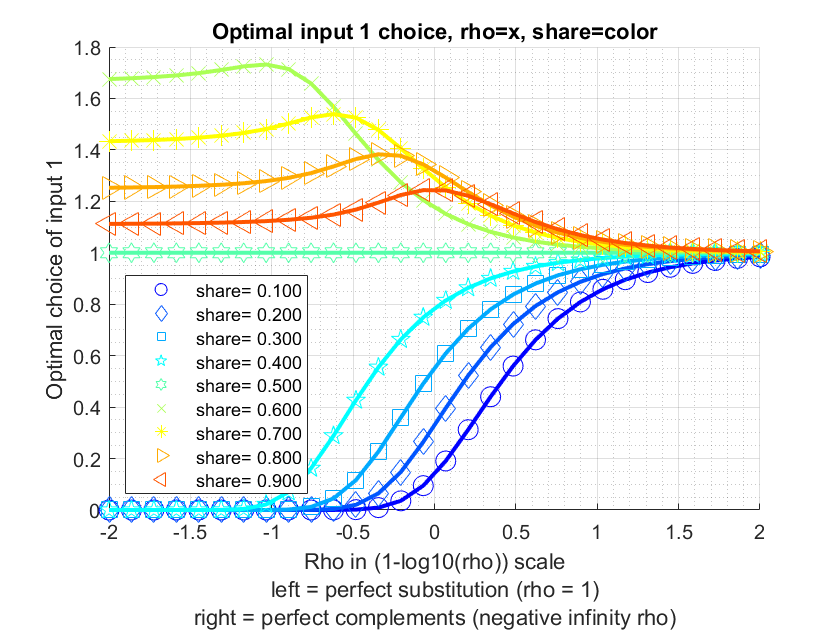
\includegraphics[width=5.20833in,height=\textheight]{img/bfwx_crs_nested_ces_images/figure_0.png}

\hypertarget{doubly-nest-layer-two-inputs-each-sub-nest-ces-problem-demand}{%
\subsection{Doubly Nest Layer Two Inputs Each Sub-nest CES Problem (Demand)}\label{doubly-nest-layer-two-inputs-each-sub-nest-ces-problem-demand}}

In this third example, solve for optimal choices for a doubly nested
problem. Below, we first solve for the optimal choices, then we do a
number of checks, to make sure that the solutions are correct, as
expected.

\begin{verbatim}
% output requirement
fl_yz = 2.1;
% upper nest 0.1, lower nests 0.35 and -1 separately for rho values
cl_mn_prho = {[0.1], [0.35, -1]};
% unequal shares of share values
cl_mn_pshare = {[0.4], [0.3, 0.88]};
% differential wages
% in lower-left nest, not productive and very expensive, not very elastic
% last index for left or right,
cl_mn_price = {[nan, nan], [10, 1;3, 4]};
% print option
bl_verbose = true;
[cl_mn_yz_choices, cl_mn_price, cl_mn_prho, cl_mn_pshare] = ...
    bfw_crs_nested_ces(fl_yz, cl_mn_prho, cl_mn_pshare, cl_mn_price, ...
    mp_func, bl_verbose, bl_bfw_model);

----------------------------------------
xxxxxxxxxxxxxxxxxxxxxxxxxxxxxxxxxxxxxxxx
CONTAINER NAME: mp_container_map ND Array (Matrix etc)
xxxxxxxxxxxxxxxxxxxxxxxxxxxxxxxxxxxxxxxx
                 i    idx    ndim    numel    rowN    colN     sum       mean       std      coefvari      min        max  
                 _    ___    ____    _____    ____    ____    ______    ______    _______    ________    ________    ______

    prho_c2      1     2      2        2       1       2       -0.65    -0.325    0.95459    -2.9372           -1      0.35
    price_c1     2     3      2        2       1       2      7.7788    3.8894     2.0959    0.53886       2.4074    5.3714
    price_c2     3     4      2        4       2       2          18       4.5      3.873    0.86066            1        10
    pshare_c2    4     6      2        2       1       2        1.18      0.59    0.41012    0.69512          0.3      0.88
    yz_c1        5     7      2        2       1       2      4.4862    2.2431    0.68863      0.307       1.7561      2.73
    yz_c2        6     8      2        4       2       2      9.0506    2.2626     2.7086     1.1971     0.047893    6.0934

xxx TABLE:prho_c2 xxxxxxxxxxxxxxxxxx
           c1     c2
          ____    __

    r1    0.35    -1

xxx TABLE:price_c1 xxxxxxxxxxxxxxxxxx
            c1        c2  
          ______    ______

    r1    2.4074    5.3714

xxx TABLE:price_c2 xxxxxxxxxxxxxxxxxx
          c1    c2
          __    __

    r1    10    1 
    r2     3    4 

xxx TABLE:pshare_c2 xxxxxxxxxxxxxxxxxx
          c1      c2 
          ___    ____

    r1    0.3    0.88

xxx TABLE:yz_c1 xxxxxxxxxxxxxxxxxx
           c1       c2  
          ____    ______

    r1    2.73    1.7561

xxx TABLE:yz_c2 xxxxxxxxxxxxxxxxxx
             c1         c2   
          ________    _______

    r1    0.047893     6.0934
    r2      2.2044    0.70496

----------------------------------------
xxxxxxxxxxxxxxxxxxxxxxxxxxxxxxxxxxxxxxxx
CONTAINER NAME: mp_container_map Scalars
xxxxxxxxxxxxxxxxxxxxxxxxxxxxxxxxxxxxxxxx
                 i    idx    value
                 _    ___    _____

    prho_c1      1     1      0.1 
    pshare_c1    2     5      0.4 

% there are four optimal choices, they are
fl_opti_x11 = cl_mn_yz_choices{2}(1,1);
fl_opti_x12 = cl_mn_yz_choices{2}(1,2);
fl_opti_x21 = cl_mn_yz_choices{2}(2,1);
fl_opti_x22 = cl_mn_yz_choices{2}(2,2);
% display
st_print = strjoin(...
    ["completed double nest test:", ...
    ['nest 1 input 1, fl_opti_x11=' num2str(fl_opti_x11)], ...
    ['nest 1 input 2, fl_opti_x12=' num2str(fl_opti_x12)], ...
    ['nest 2 input 1, fl_opti_x21=' num2str(fl_opti_x21)], ...
    ['nest 2 input 2, fl_opti_x22=' num2str(fl_opti_x22)], ...
    ], ";");
st_out = st_print;
ar_ch_out = char(strsplit(st_print,";")');
disp(ar_ch_out);

completed double nest test:         
nest 1 input 1, fl_opti_x11=0.047893
nest 1 input 2, fl_opti_x12=6.0934  
nest 2 input 1, fl_opti_x21=2.2044  
nest 2 input 2, fl_opti_x22=0.70496 
\end{verbatim}

\hypertarget{doubly-nest-layer-two-inputs-each-sub-nest-ces-problemsolution-check-demand}{%
\subsection{Doubly Nest Layer Two Inputs Each Sub-nest CES Problem--Solution Check (Demand)}\label{doubly-nest-layer-two-inputs-each-sub-nest-ces-problemsolution-check-demand}}

Checking output equality, if there are problems, would output an error.

\begin{verbatim}
% A. Check output Equality
fl_pshare_0 = cl_mn_pshare{1}(1);
fl_pshare_1 = cl_mn_pshare{2}(1);
fl_pshare_2 = cl_mn_pshare{2}(2);
fl_prho_0 = cl_mn_prho{1}(1);
fl_prho_1 = cl_mn_prho{2}(1);
fl_prho_2 = cl_mn_prho{2}(2);
fl_output_1 = ((fl_pshare_1)*fl_opti_x11^(fl_prho_1) + (1-fl_pshare_1)*fl_opti_x12^(fl_prho_1))^(1/fl_prho_1);
fl_output_2 = ((fl_pshare_2)*fl_opti_x21^(fl_prho_2) + (1-fl_pshare_2)*fl_opti_x22^(fl_prho_2))^(1/fl_prho_2);
fl_output_0 = ((fl_pshare_0)*fl_output_1^(fl_prho_0) + (1-fl_pshare_0)*fl_output_2^(fl_prho_0))^(1/fl_prho_0);
if (~if_is_close(fl_output_0, fl_yz))
    error('There is an error, output is not equal to required expenditure minimizing output')
end
\end{verbatim}

Checking FOC within-nest optimality, if there are problems, would output
an error.

\begin{verbatim}
% B. Check FOC Optimality inner nest
fl_wage_x11 = cl_mn_price{2}(1,1);
fl_wage_x12 = cl_mn_price{2}(1,2);
fl_wage_x21 = cl_mn_price{2}(2,1);
fl_wage_x22 = cl_mn_price{2}(2,2);

% B1. Checking via Method 1
fl_rela_opti_foc_1 = (((fl_pshare_1/(1-fl_pshare_1)))*(fl_wage_x12/fl_wage_x11))^(1/(1-fl_prho_1));
fl_rela_opti_foc_2 = (((fl_pshare_2/(1-fl_pshare_2)))*(fl_wage_x22/fl_wage_x21))^(1/(1-fl_prho_2));
if (~if_is_close(fl_rela_opti_foc_1, fl_opti_x11/fl_opti_x12))
    error('B1. There is an error, optimal relative not equal to expected foc ratio, nest 1')
end
if (~if_is_close(fl_rela_opti_foc_2, fl_opti_x21/fl_opti_x22))
    error('B1. There is an error, optimal relative not equal to expected foc ratio, nest 2')
end

% B2. Equation left to right, right to left, checking via method 2
% Check FOC Optimality cross nests (actually within) T1
fl_dy_dx11 = fl_pshare_1*(fl_opti_x11^(fl_prho_1-1));
fl_dy_dx12 = (1-fl_pshare_1)*(fl_opti_x12^(fl_prho_1-1));
fl_rwage_x11dx12 = fl_dy_dx11/fl_dy_dx12;
if (~if_is_close(fl_rwage_x11dx12, fl_wage_x11/fl_wage_x12))
    error('B2. There is an error, relative price x11 and x12 does not satisfy within optimality across nests')
end
\end{verbatim}

Generate aggregate prices, if there are problems, would output an error.

\begin{verbatim}
% C. Aggregate prices and optimality within higher tier
% Is optimality satisfied given aggregate prices?
fl_rela_wage_share_11 = ...
    ((fl_wage_x11/fl_wage_x12)*((1-fl_pshare_1)/(fl_pshare_1)))^(fl_prho_1/(1-fl_prho_1));
fl_rela_wage_share_12 = ...
    ((fl_wage_x12/fl_wage_x11)*((fl_pshare_1)/(1-fl_pshare_1)))^(fl_prho_1/(1-fl_prho_1));
fl_agg_prc_1 = ...
    fl_wage_x11*(fl_pshare_1 + (1-fl_pshare_1)*(fl_rela_wage_share_11))^(-1/fl_prho_1) + ...
    fl_wage_x12*(fl_pshare_1*(fl_rela_wage_share_12) + (1-fl_pshare_1))^(-1/fl_prho_1);

fl_rela_wage_share_21 = ...
    ((fl_wage_x21/fl_wage_x22)*((1-fl_pshare_2)/(fl_pshare_2)))^(fl_prho_2/(1-fl_prho_2));
fl_rela_wage_share_22 = ...
    ((fl_wage_x22/fl_wage_x21)*((fl_pshare_2)/(1-fl_pshare_2)))^(fl_prho_2/(1-fl_prho_2));
fl_agg_prc_2 = ...
    fl_wage_x21*(fl_pshare_2 + (1-fl_pshare_2)*(fl_rela_wage_share_21))^(-1/fl_prho_2) + ...
    fl_wage_x22*(fl_pshare_2*(fl_rela_wage_share_22) + (1-fl_pshare_2))^(-1/fl_prho_2);

% What is returned by the omega function that is suppose to have aggregate prices?
mp_func = bfw_mp_func_demand();
params_group = values(mp_func, {'fc_OMEGA', 'fc_d1', 'fc_d2'});
[fc_OMEGA, fc_d1, fc_d2] = params_group{:};

% Aggregate price
fl_aggregate_price_1 = fc_OMEGA(...
    fl_wage_x11, fl_wage_x12, ...
    fl_prho_1, ...
    fl_pshare_1, 1 - fl_pshare_1);

fl_aggregate_price_2 = fc_OMEGA(...
    fl_wage_x21, fl_wage_x22, ...
    fl_prho_2, ...
    fl_pshare_2, 1 - fl_pshare_2);    
\end{verbatim}

Check relative price within nest and across nests, if there are
problems, would output an error.

\begin{verbatim}
% D. Check FOC Optimality cross nests

% D1a. Two within-nest relative wages and four cross-nest relative wages
% within
fl_rwage_x11dx12 = fl_wage_x11/fl_wage_x12;
fl_rwage_x21dx22 = fl_wage_x21/fl_wage_x22;
% across
fl_rwage_x11dx21 = fl_wage_x11/fl_wage_x21;
fl_rwage_x11dx22 = fl_wage_x11/fl_wage_x22;
fl_rwage_x12dx21 = fl_wage_x12/fl_wage_x21;
fl_rwage_x12dx22 = fl_wage_x12/fl_wage_x22;

% D1b. Generate relative wages within nest and across nests own equations
fl_dy_dx1_shared = (fl_pshare_0*(fl_output_1)^(fl_prho_0-1))*((fl_output_1)^(1-fl_prho_1));
fl_dy_dx11 = fl_dy_dx1_shared*(fl_pshare_1*fl_opti_x11^(fl_prho_1-1));
fl_dy_dx12 = fl_dy_dx1_shared*((1-fl_pshare_1)*fl_opti_x12^(fl_prho_1-1));

fl_dy_dx2_shared = ((1-fl_pshare_0)*(fl_output_2)^(fl_prho_0-1))*((fl_output_2)^(1-fl_prho_2));
fl_dy_dx21 = fl_dy_dx2_shared*(fl_pshare_2*fl_opti_x21^(fl_prho_2-1));
fl_dy_dx22 = fl_dy_dx2_shared*((1-fl_pshare_2)*fl_opti_x22^(fl_prho_2-1));

% within
fl_rwage_x11dx12_foc = fl_dy_dx11/fl_dy_dx12;
fl_rwage_x21dx22_foc = fl_dy_dx21/fl_dy_dx22;
% across
fl_rwage_x11dx21_foc = fl_dy_dx11/fl_dy_dx21;
fl_rwage_x11dx22_foc = fl_dy_dx11/fl_dy_dx22;
fl_rwage_x12dx21_foc = fl_dy_dx12/fl_dy_dx21;
fl_rwage_x12dx22_foc = fl_dy_dx12/fl_dy_dx22;

if (~if_is_close(fl_rwage_x11dx21_foc, fl_wage_x11/fl_wage_x21))
    error('There is an error, relative price x11 and x21 does not satisfy cross optimality across nests')
end
if (~if_is_close(fl_rwage_x12dx22_foc, fl_wage_x12/fl_wage_x22))
    error('There is an error, relative price x12 and x22 does not satisfy cross optimality across nests')
end

% D2. Check FOC Optimality cross nests, simplified equation
fl_rela_wage_x11_x21 = log((fl_pshare_0/(1-fl_pshare_0))* ...
    ((fl_pshare_1*fl_opti_x11^(fl_prho_1-1)*fl_output_2^(fl_prho_2))/(fl_pshare_2*fl_opti_x21^(fl_prho_2-1)*fl_output_1^(fl_prho_1)))) + ...
    fl_prho_0*log(fl_output_1/fl_output_2);
if (~if_is_close(fl_rela_wage_x11_x21, log(fl_wage_x11/fl_wage_x21)))
    error('There is an error, relative price x11 and x21 does not satisfy cross optimality across nests')
end
\end{verbatim}

\hypertarget{bfw-2022-nested-three-branch-four-layer-problem-demand}{%
\subsection{BFW (2022) Nested Three Branch (Four Layer) Problem (Demand)}\label{bfw-2022-nested-three-branch-four-layer-problem-demand}}

The model BFW 2022 has three branches and four layers. one of the
branches go down only three layers, the other two branches go down four
layers.

First, we prepare the various inputs:

\begin{verbatim}
% Controls
bl_verbose = true;
bl_bfw_model = true;

% Given rho and beta, solve for equilibrium quantities
bl_log_wage = false;
mp_func = bfw_mp_func_demand(bl_log_wage);

% Following instructions in: PrjFLFPMexicoBFW\solvedemand\README.md

% Nests/layers
it_nests = 4;

% Input cell of mn matrixes
it_prho_cl = 1;
it_pshare_cl = 2;
it_price_cl = 3;
for it_cl_ctr = [1,2,3]

    cl_mn_cur = cell(it_nests,1);

    % Fill each cell element with NaN mn array
    for it_cl_mn = 1:it_nests

        bl_price = (it_cl_ctr == it_price_cl);

        if (~bl_price && it_cl_mn == 1)
            mn_nan = NaN;
        elseif (~bl_price && it_cl_mn == 2) || (bl_price && it_cl_mn == 1)
            mn_nan = [NaN, NaN];
        elseif (~bl_price && it_cl_mn == 3) || (bl_price && it_cl_mn == 2)
            mn_nan = NaN(2,2);
        elseif (~bl_price && it_cl_mn == 4) || (bl_price && it_cl_mn == 3)
            mn_nan = NaN(2,2,2);
        elseif (~bl_price && it_cl_mn == 5) || (bl_price && it_cl_mn == 4)
            mn_nan = NaN(2,2,2,2);
        elseif (~bl_price && it_cl_mn == 6) || (bl_price && it_cl_mn == 5)
            mn_nan = NaN(2,2,2,2,2);
        end
        cl_mn_cur{it_cl_mn} = mn_nan;
    end

    % Name cell arrays
    if (it_cl_ctr == it_prho_cl)
        cl_mn_prho = cl_mn_cur;
    elseif (it_cl_ctr == it_pshare_cl)
        cl_mn_pshare = cl_mn_cur;
    elseif (it_cl_ctr == it_price_cl)
        cl_mn_price = cl_mn_cur;
    end
end

% Initialize share matrix
rng(123);
for it_cl_mn = 1:it_nests
    mn_pshare = cl_mn_pshare{it_cl_mn};
    if it_cl_mn == 4
        mn_pshare(2,:,:) = rand(2,2);
    else
        mn_pshare = rand(size(mn_pshare));
    end
    cl_mn_pshare{it_cl_mn} = mn_pshare;
end

% Initialize rho matrix
rng(456);
for it_cl_mn = 1:it_nests
    mn_prho = cl_mn_prho{it_cl_mn};
    if it_cl_mn == 4
        mn_prho(2,:,:) = rand(2,2);
    else
        mn_prho = rand(size(mn_prho));
    end
    % Scalling rho between 0.7500 and -3.0000
    % 1 - 2.^(linspace(-2,2,5))
    mn_prho = 1 - 2.^(mn_prho*(4) - 2);
    cl_mn_prho{it_cl_mn} = mn_prho;
end

% Initialize wage matrix
rng(789);
for it_cl_mn = 1:it_nests
    mn_price = cl_mn_price{it_cl_mn};
    if it_cl_mn == 3
        mn_price(1,:,:) = rand(2,2);
    elseif it_cl_mn == 4
        mn_price(2,:,:,:) = rand(2,2,2);
    end
    % Scalling rho between 3 amd 5
    mn_price = mn_price*(2) + 3;
    cl_mn_price{it_cl_mn} = mn_price;
end

% Initialize yz matrix
rng(101112);
fl_yz = rand();
\end{verbatim}

Second, display created inputs:

\begin{verbatim}
disp(['fl_yz=' num2str(fl_yz)]);

fl_yz=0.89726

celldisp(cl_mn_prho);


cl_mn_prho{1} =
 
    0.5017



cl_mn_prho{2} =
 
    0.6071   -1.1955



cl_mn_prho{3} =
 
   -1.3523   -0.3346
   -0.4167   -1.9136



cl_mn_prho{4} =
 

(:,:,1) =

       NaN       NaN
   -1.0512    0.5869


(:,:,2) =

       NaN       NaN
    0.6209    0.1633



celldisp(cl_mn_pshare);


cl_mn_pshare{1} =
 
    0.6965



cl_mn_pshare{2} =
 
    0.2861    0.2269



cl_mn_pshare{3} =
 
    0.5513    0.4231
    0.7195    0.9808



cl_mn_pshare{4} =
 

(:,:,1) =

       NaN       NaN
    0.6848    0.4809


(:,:,2) =

       NaN       NaN
    0.3921    0.3432



celldisp(cl_mn_price);


cl_mn_price{1} =
 
   NaN   NaN



cl_mn_price{2} =
 
   NaN   NaN
   NaN   NaN



cl_mn_price{3} =
 

(:,:,1) =

    3.6467    3.4605
       NaN       NaN


(:,:,2) =

    4.5876    4.2488
       NaN       NaN



cl_mn_price{4} =
 

(:,:,1,1) =

       NaN       NaN
    4.9508    4.5178


(:,:,2,1) =

       NaN       NaN
    3.0212    3.0495


(:,:,1,2) =

       NaN       NaN
    3.2221    4.0763


(:,:,2,2) =

       NaN       NaN
    3.0909    4.1031
\end{verbatim}

Third, call function and solve for optimal demand:

\begin{verbatim}
% Call function
[cl_mn_yz_choices, cl_mn_price, cl_mn_prho, cl_mn_pshare] = ...
    bfw_crs_nested_ces(fl_yz, cl_mn_prho, cl_mn_pshare, cl_mn_price, ...
    mp_func, bl_verbose, bl_bfw_model);

----------------------------------------
xxxxxxxxxxxxxxxxxxxxxxxxxxxxxxxxxxxxxxxx
CONTAINER NAME: mp_container_map ND Array (Matrix etc)
xxxxxxxxxxxxxxxxxxxxxxxxxxxxxxxxxxxxxxxx
                            i     idx    ndim    numel    rowN    colN      sum         mean        std       coefvari      min         max   
                            __    ___    ____    _____    ____    ____    ________    ________    ________    ________    ________    ________

    mt_fl_labor_demanded     1     1      2       12       4       3        5.4455     0.45379     0.85359       1.881    0.020122      2.3642
    prho_c2                  2     3      2        2       1       2      -0.58844    -0.29422      1.2746     -4.3323     -1.1955     0.60709
    prho_c3                  3     4      2        4       2       2       -4.0173     -1.0043     0.76195    -0.75868     -1.9136    -0.33464
    prho_c4                  4     5      3        8       2       4           NaN         NaN         NaN         NaN     -1.0512     0.62089
    price_c1                 5     6      2        2       1       2        35.345      17.673      7.0394     0.39832      12.695       22.65
    price_c2                 6     7      2        4       2       2        40.906      10.226      2.7834     0.27217      7.7015      13.522
    price_c3                 7     8      3        8       2       4        45.403      5.6754      2.0037     0.35305      3.4605      8.5114
    price_c4                 8     9      4       16       2       8           NaN         NaN         NaN         NaN      3.0212      4.9508
    pshare_c2                9    11      2        2       1       2       0.51299      0.2565    0.041923     0.16344     0.22685     0.28614
    pshare_c3               10    12      2        4       2       2        2.6747     0.66866     0.24087     0.36023     0.42311     0.98076
    pshare_c4               11    13      3        8       2       4           NaN         NaN         NaN         NaN     0.34318     0.68483
    yz_c1                   12    14      2        2       1       2        1.6003     0.80016      1.0053      1.2564    0.089284       1.511
    yz_c2                   13    15      2        4       2       2         2.645     0.66124      1.0849      1.6407    0.057461      2.2864
    yz_c3                   14    16      3        8       2       4        5.1962     0.64953      1.0063      1.5492     0.03298      2.3642
    yz_c4                   15    17      4       16       2       8           NaN         NaN         NaN         NaN    0.020122     0.14469

xxx TABLE:mt_fl_labor_demanded xxxxxxxxxxxxxxxxxx
             c1          c2         c3   
          ________    ________    _______

    r1    0.020122    0.024929     2.1857
    r2    0.060227    0.037985     2.3642
    r3    0.069088    0.093774    0.21107
    r4    0.058349     0.14469    0.17539

xxx TABLE:prho_c2 xxxxxxxxxxxxxxxxxx
            c1         c2   
          _______    _______

    r1    0.60709    -1.1955

xxx TABLE:prho_c3 xxxxxxxxxxxxxxxxxx
             c1          c2   
          ________    ________

    r1     -1.3523    -0.33464
    r2    -0.41668     -1.9136

xxx TABLE:prho_c4 xxxxxxxxxxxxxxxxxx
            c1         c2         c3         c4   
          _______    _______    _______    _______

    r1        NaN        NaN        NaN        NaN
    r2    -1.0512    0.58694    0.62089    0.16334

xxx TABLE:price_c1 xxxxxxxxxxxxxxxxxx
            c1       c2  
          ______    _____

    r1    12.695    22.65

xxx TABLE:price_c2 xxxxxxxxxxxxxxxxxx
            c1        c2  
          ______    ______

    r1    8.1518    7.7015
    r2    13.522     11.53

xxx TABLE:price_c3 xxxxxxxxxxxxxxxxxx
            c1        c2        c3        c4  
          ______    ______    ______    ______

    r1    3.6467    3.4605    4.5876    4.2488
    r2    8.1184    8.5114    5.7986    7.0309

xxx TABLE:price_c4 xxxxxxxxxxxxxxxxxx
            c1        c2        c3        c4        c5        c6        c7        c8  
          ______    ______    ______    ______    ______    ______    ______    ______

    r1       NaN       NaN       NaN       NaN       NaN       NaN       NaN       NaN
    r2    4.9508    4.5178    3.0212    3.0495    3.2221    4.0763    3.0909    4.1031

xxx TABLE:pshare_c2 xxxxxxxxxxxxxxxxxx
            c1         c2   
          _______    _______

    r1    0.28614    0.22685

xxx TABLE:pshare_c3 xxxxxxxxxxxxxxxxxx
            c1         c2   
          _______    _______

    r1    0.55131    0.42311
    r2    0.71947    0.98076

xxx TABLE:pshare_c4 xxxxxxxxxxxxxxxxxx
            c1         c2         c3         c4   
          _______    _______    _______    _______

    r1        NaN        NaN        NaN        NaN
    r2    0.68483    0.48093    0.39212    0.34318

xxx TABLE:yz_c1 xxxxxxxxxxxxxxxxxx
           c1         c2   
          _____    ________

    r1    1.511    0.089284

xxx TABLE:yz_c2 xxxxxxxxxxxxxxxxxx
             c1         c2  
          ________    ______

    r1     0.19312    2.2864
    r2    0.057461     0.108

xxx TABLE:yz_c3 xxxxxxxxxxxxxxxxxx
            c1         c2          c3         c4   
          _______    _______    ________    _______

    r1    0.21107     2.1857     0.17539     2.3642
    r2    0.06529    0.11907    0.042587    0.03298

xxx TABLE:yz_c4 xxxxxxxxxxxxxxxxxx
             c1          c2          c3          c4          c5         c6          c7          c8   
          ________    ________    ________    ________    ________    _______    ________    ________

    r1         NaN         NaN         NaN         NaN         NaN        NaN         NaN         NaN
    r2    0.069088    0.093774    0.020122    0.024929    0.058349    0.14469    0.060227    0.037985

----------------------------------------
xxxxxxxxxxxxxxxxxxxxxxxxxxxxxxxxxxxxxxxx
CONTAINER NAME: mp_container_map Scalars
xxxxxxxxxxxxxxxxxxxxxxxxxxxxxxxxxxxxxxxx
                 i    idx     value 
                 _    ___    _______

    prho_c1      1     2     0.50172
    pshare_c1    2    10     0.69647
\end{verbatim}

\hypertarget{compute-nested-ces-mpl-given-demand-crs}{%
\section{Compute Nested CES MPL Given Demand (CRS)}\label{compute-nested-ces-mpl-given-demand-crs}}

Testing the
\href{https://github.com/FanWangEcon/PrjLabEquiBFW/blob/main/PrjLabEquiBFW/solvedemand/bfw_crs_nested_ces_mpl.m}{\textbf{bfw\_crs\_nested\_ces\_mpl}}
function from the \href{https://fanwangecon.github.io/PrjLabEquiBFW/}{\textbf{PrjLabEquiBFW
Package}}\textbf{.} Given
labor quantity demanded, using first-order relative optimality
conditions, find the marginal product of labor given CES production
function. Results match up with correct relative wages, but not wage
levels. Takes as inputs share and elasticity parameters across layers of
sub-nests, as well as quantity demanded at each bottom-most CES nest
layer. Works with Constant Elasticity of Substitution problems with
constant returns, up to four nest layers, and two inputs in each
sub-nest. Allows for uneven branches, so that some branches go up to
four layers, but others have less layers, works with BFW (2022) nested
labor input problem.

\hypertarget{key-inputs-and-outputs-for-bfw_crs_nested_ces_mpl}{%
\subsection{\texorpdfstring{Key Inputs and Outputs for \href{https://github.com/FanWangEcon/PrjLabEquiBFW/blob/main/PrjLabEquiBFW/solvedemand/bfw_crs_nested_ces_mpl.m}{\textbf{bfw\_crs\_nested\_ces\_mpl}}}{Key Inputs and Outputs for bfw\_crs\_nested\_ces\_mpl}}\label{key-inputs-and-outputs-for-bfw_crs_nested_ces_mpl}}

Here are the key inputs for the CES demand solver function:

\begin{itemize}
\item
  \textbf{CL\_MN\_PRHO} cell array of rho (elasticity) parameter between
  negative infinity and 1. For example, suppose there are four nest
  layers, and there are two branches at each layer, then we have 1, 2,
  4, and 8 \(\rho\) parameter values at the 1st, 2nd, 3rd, and 4th nest
  layers: size(CL\_MN\_PRHO\{1\})= \(\left\lbrack 1,1\right\rbrack\),
  size(CL\_MN\_PRHO\{2\}) = \(\left\lbrack 1,2\right\rbrack\),
  size(CL\_MN\_PRHO\{3\}) = \(\left\lbrack 2,2\right\rbrack\),
  size(CL\_MN\_PRHO\{4\}) = \(\left\lbrack 2,2,2\right\rbrack\). Note that
  if the model has 4 nest layers, not all cells need to be specified,
  some branches could be deeper than others.
\item
  \textbf{CL\_MN\_PSHARE} cell array of share (between 0 and 1) for the first
  input of the two inputs for each nest. The structure for this is
  similar to CL\_MN\_PRHO.
\item
  \textbf{CL\_MN\_YZ\_CHOICES} cell array of quantity demanded for the first
  and second inputs of the bottom-most layer of sub-nests. The last
  index in each element of the cell array indicates first (1) or
  second (2) quantities. For example, suppose we have four layers,
  with 2 branches at each layer, as in the example for CL\_MN\_PRHO,
  then we have 2, 4, 8, and 16 quantity values at the 1st, 2nd, 3rd,
  and 4th nest layers: size(CL\_MN\_YZ\_CHOICES\{1\})=
  \(\left\lbrack 1,2\right\rbrack\), size(CL\_MN\_YZ\_CHOICES\{2\})=
  \(\left\lbrack 2,2\right\rbrack\), size(CL\_MN\_YZ\_CHOICES\{3\})=
  \(\left\lbrack 2,2,2\right\rbrack\), size(CL\_MN\_YZ\_CHOICES\{4\})=
  \(\left\lbrack 2,2,2,2\right\rbrack\). Note that only the last layer
  of quantities needs to be specified, in this case, the 16 quantities
  at the 4th layer. Given first order conditions, we solve for the 2,
  4, and 8 aggregate quantities at the higher nest layers. If some
  branches are deeper than other branches, then can specific NA for
  non-reached layers along some branches.
\item
  \textbf{BL\_BFW\_MODEL} boolean true by default if true then will output
  outcomes specific to the BFW 2022 problem.
\end{itemize}

Here are the key outputs for the CES demand solver function:

\begin{itemize}
\item
  \textbf{CL\_MN\_MPL\_PRICE} has the same dimension as CL\_MN\_YZ\_CHOICES,
  suppose there are four layers, the CL\_MN\_MPL\_PRICE\{4\} results at the
  lowest layer includes wages that might be observed in the data.
  CL\_MN\_MPL\_PRICE cell values at non-bottom layers include aggregate
  wages.
\item
  \textbf{CL\_MN\_YZ\_CHOICES} includes at the lowest layer observed wages,
  however, also includes higher layer aggregate solved quantities.
  CL\_MN\_PRHO and CL\_MN\_PSHARE are identical to inputs.
\end{itemize}

\hypertarget{single-nest-layer-two-inputs-ces-problem-mpl}{%
\subsection{Single Nest Layer Two Inputs CES Problem (MPL)}\label{single-nest-layer-two-inputs-ces-problem-mpl}}

In this first example, we solve a constant returns to scale problem with
a single nest, meaning just two inputs and a single output.

\begin{verbatim}
clc;
close all;
clear all;

% rho = 0.5, 1/(1-0.5)=2, elasticity of substitution of 2
cl_mn_prho = {[0.1]};
% equal share, similar "productivity"
cl_mn_pshare = {[0.5]};
% levels of the two inputs, Values picked from demand problem parallel
% example.
cl_mn_yz_choices = {[0.67537, 1.4589]};
% print option
bl_verbose = true;
mp_func = bfw_mp_func_demand();
bl_bfw_model = false;
[cl_mn_yz_choices, cl_mn_mpl_price] = ...
    bfw_crs_nested_ces_mpl(cl_mn_prho, cl_mn_pshare, cl_mn_yz_choices, ...
    mp_func, bl_verbose, bl_bfw_model);

----------------------------------------
xxxxxxxxxxxxxxxxxxxxxxxxxxxxxxxxxxxxxxxx
CONTAINER NAME: mp_container_map ND Array (Matrix etc)
xxxxxxxxxxxxxxxxxxxxxxxxxxxxxxxxxxxxxxxx
                    i    idx    ndim    numel    rowN    colN     sum       mean        std      coefvari      min        max  
                    _    ___    ____    _____    ____    ____    ______    _______    _______    ________    _______    _______

    mpl_price_c1    1     1      2        2       1       2      1.0678    0.53388    0.25168    0.47141     0.35592    0.71184
    yz_c1           2     4      2        2       1       2      2.1343     1.0671    0.55404    0.51918     0.67537     1.4589

xxx TABLE:mpl_price_c1 xxxxxxxxxxxxxxxxxx
            c1         c2   
          _______    _______

    r1    0.71184    0.35592

xxx TABLE:yz_c1 xxxxxxxxxxxxxxxxxx
            c1         c2  
          _______    ______

    r1    0.67537    1.4589

----------------------------------------
xxxxxxxxxxxxxxxxxxxxxxxxxxxxxxxxxxxxxxxx
CONTAINER NAME: mp_container_map Scalars
xxxxxxxxxxxxxxxxxxxxxxxxxxxxxxxxxxxxxxxx
                 i    idx    value
                 _    ___    _____

    prho_c1      1     2      0.1 
    pshare_c1    2     3      0.5 
\end{verbatim}

\hypertarget{single-nest-layer-two-inputs-ces-problem-vary-share-and-elasticity-mpl}{%
\subsection{Single Nest Layer Two Inputs CES Problem, Vary Share and Elasticity (MPL)}\label{single-nest-layer-two-inputs-ces-problem-vary-share-and-elasticity-mpl}}

In this second example, we test over different rho values, explore
optimal relative choices, as share and elasticity change. In this
exercise, we also check, at every combination of rho and share
parameter, whether the FOC condition is satisfied by the optimal
choices. Also check if at the optimal choices, the minimization output
requirement is met.

\begin{verbatim}
% Approximately close function
rel_tol=1e-09;
abs_tol=0.0;
if_is_close = @(a,b) (abs(a-b) <= max(rel_tol * max(abs(a), abs(b)), abs_tol));

% Input 1 and 2 fixed
fl_x_1 = 0.95;
fl_x_2 = 1.05;

% Define share and rho arrays
ar_pshare = linspace(0.1, 0.9, 9);
ar_prho = 1 - 10.^(linspace(-2, 2, 30));
% Loop over share and rho values
mt_rela_opti = NaN([length(ar_pshare), length(ar_prho)]);
mt_rela_wage = NaN([length(ar_pshare), length(ar_prho)]);
for it_pshare_ctr = 1:length(ar_pshare)
    for it_prho_ctr = 1:length(ar_prho)

        % A. Parameters
        % rho
        fl_prho = ar_prho(it_prho_ctr);
        cl_mn_prho = {[fl_prho]};
        % share
        fl_pshare = ar_pshare(it_pshare_ctr);
        cl_mn_pshare = {[fl_pshare]};
        % wages for the two inputs, identical wage
        % Note that if chosee {[1,1]} below, log(1/1) = log(1) = 0,
        % elasticity does not matter. 
        cl_mn_yz_choices = {[fl_x_1, fl_x_2]};
        % print option
        bl_verbose = false;

        % B. Call function
        [cl_mn_yz_choices, cl_mn_mpl_price] = ...
            bfw_crs_nested_ces_mpl(cl_mn_prho, cl_mn_pshare, cl_mn_yz_choices, ...
            mp_func, bl_verbose, bl_bfw_model);
        % Store results for mpl given input choices
        fl_mpl_x1 = cl_mn_mpl_price{1}(1);
        fl_mpl_x2 = cl_mn_mpl_price{1}(2);
        mt_rela_wage(it_pshare_ctr, it_prho_ctr) = log(fl_mpl_x1/fl_mpl_x2);
    end
end
\end{verbatim}

Key results: (1) As share parameter of input 1 goes to zero, input 1 is
less productive, and the log(mplx1/mplx2) ratio is lower. (2) Becaus x2
input in this example is larger than x1 input, so as two inputs become
more inelastic (more leontief), relative MPL for the lower level input
is now larger. At the Leontief extreme, the MPL of the input provided at
lower level is infinity.

\begin{verbatim}
% Visualize
% Generate some Data
rng(456);
ar_row_grid = ar_pshare;
ar_col_grid = log(1-ar_prho)/log(10);
rng(123);
mt_value = mt_rela_wage;
% container map settings
mp_support_graph = containers.Map('KeyType', 'char', 'ValueType', 'any');
mp_support_graph('cl_st_graph_title') = {...
    ['Log Relative MPL/Wages, rho=x, share=color'] ...
    ['input x1 = ' num2str(fl_x_1) ' input x2 = ' num2str(fl_x_2)]
    };
mp_support_graph('cl_st_ytitle') = {'Log(mplx1/mplx2)'};
mp_support_graph('cl_st_xtitle') = {'Rho in (1-log10(rho)) scale', ...
    'left = perfect substitution (rho = 1)', ...
    'right = perfect complements (negative infinity rho)'};
mp_support_graph('st_legend_loc') = 'best';
mp_support_graph('bl_graph_logy') = false; % do not log
mp_support_graph('st_rowvar_name') = 'share=';
mp_support_graph('it_legend_select') = 5; % how many shock legends to show
mp_support_graph('st_rounding') = '6.3f'; % format shock legend
mp_support_graph('cl_colors') = 'jet'; % any predefined matlab colormap
% Call function
ff_graph_grid(mt_value, ar_row_grid, ar_col_grid, mp_support_graph);
\end{verbatim}

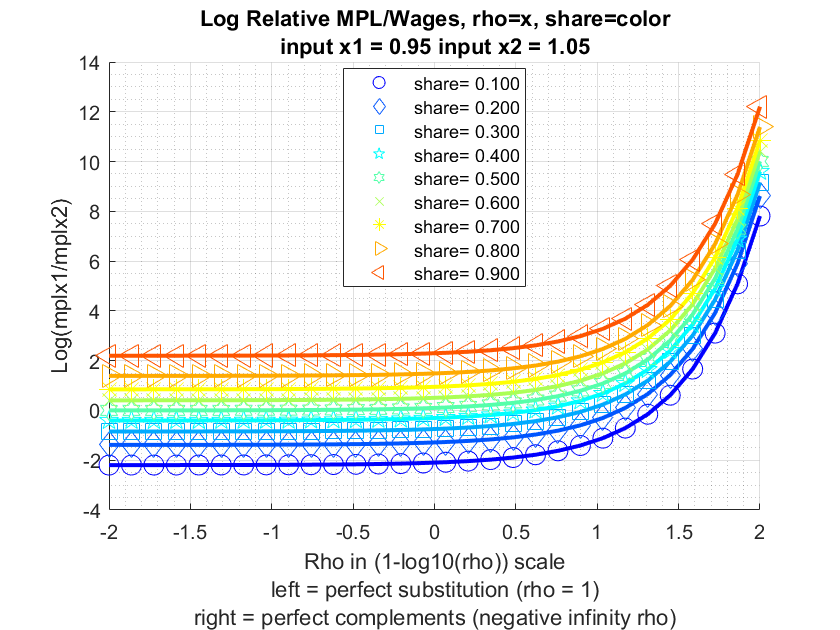
\includegraphics[width=5.20833in,height=\textheight]{img/bfwx_crs_nested_ces_mpl_images/figure_0.png}

\hypertarget{doubly-nest-layer-two-inputs-each-sub-nest-ces-problem}{%
\subsection{Doubly Nest Layer Two Inputs Each Sub-nest CES Problem}\label{doubly-nest-layer-two-inputs-each-sub-nest-ces-problem}}

In this third example, solve for optimal choices for a doubly nested
problem. Below, we first solve for the optimal choices, then we do a
number of checks, to make sure that the solutions are correct, as
expected.

\begin{verbatim}
% output requirement
fl_yz = 2.1;
% upper nest 0.1, lower nests 0.35 and -1 separately for rho values
cl_mn_prho = {[0.1], [0.35, -1]};
% unequal shares of share values
cl_mn_pshare = {[0.4], [0.3, 0.88]};
% differential wages
% in lower-left nest, not productive and very expensive, not very elastic
% last index for left or right. Values picked from demand problem parallel
% example.
cl_mn_yz_choices = {[nan, nan], [0.04789, 6.0934; 2.2044, 0.70496]};
% print option
bl_verbose = true;
[cl_mn_yz_choices, cl_mn_mpl_price] = ...
    bfw_crs_nested_ces_mpl(cl_mn_prho, cl_mn_pshare, cl_mn_yz_choices, ...
    mp_func, bl_verbose, bl_bfw_model);

----------------------------------------
xxxxxxxxxxxxxxxxxxxxxxxxxxxxxxxxxxxxxxxx
CONTAINER NAME: mp_container_map ND Array (Matrix etc)
xxxxxxxxxxxxxxxxxxxxxxxxxxxxxxxxxxxxxxxx
                    i    idx    ndim    numel    rowN    colN     sum       mean        std      coefvari      min        max  
                    _    ___    ____    _____    ____    ____    ______    _______    _______    ________    _______    _______

    mpl_price_c1    1     1      2        2       1       2      1.0206    0.51032    0.27499    0.53886     0.31587    0.70476
    mpl_price_c2    2     2      2        4       2       2      2.3618    0.59045     0.5082    0.86069     0.13121     1.3121
    prho_c2         3     4      2        2       1       2       -0.65     -0.325    0.95459    -2.9372          -1       0.35
    pshare_c2       4     6      2        2       1       2        1.18       0.59    0.41012    0.69512         0.3       0.88
    yz_c1           5     7      2        2       1       2      4.4862     2.2431    0.68863      0.307      1.7562       2.73
    yz_c2           6     8      2        4       2       2      9.0507     2.2627     2.7086     1.1971     0.04789     6.0934

xxx TABLE:mpl_price_c1 xxxxxxxxxxxxxxxxxx
            c1         c2   
          _______    _______

    r1    0.31587    0.70476

xxx TABLE:mpl_price_c2 xxxxxxxxxxxxxxxxxx
            c1         c2   
          _______    _______

    r1     1.3121    0.13121
    r2    0.39362    0.52484

xxx TABLE:prho_c2 xxxxxxxxxxxxxxxxxx
           c1     c2
          ____    __

    r1    0.35    -1

xxx TABLE:pshare_c2 xxxxxxxxxxxxxxxxxx
          c1      c2 
          ___    ____

    r1    0.3    0.88

xxx TABLE:yz_c1 xxxxxxxxxxxxxxxxxx
           c1       c2  
          ____    ______

    r1    2.73    1.7562

xxx TABLE:yz_c2 xxxxxxxxxxxxxxxxxx
            c1         c2   
          _______    _______

    r1    0.04789     6.0934
    r2     2.2044    0.70496

----------------------------------------
xxxxxxxxxxxxxxxxxxxxxxxxxxxxxxxxxxxxxxxx
CONTAINER NAME: mp_container_map Scalars
xxxxxxxxxxxxxxxxxxxxxxxxxxxxxxxxxxxxxxxx
                 i    idx    value
                 _    ___    _____

    prho_c1      1     3      0.1 
    pshare_c1    2     5      0.4 

% there are four optimal choices, they are
fl_mpl_x11 = cl_mn_mpl_price{2}(1,1);
fl_mpl_x12 = cl_mn_mpl_price{2}(1,2);
fl_mpl_x21 = cl_mn_mpl_price{2}(2,1);
fl_mpl_x22 = cl_mn_mpl_price{2}(2,2);
% display
st_print = strjoin(...
    ["completed double nest test:", ...
    ['nest 1 input 1, fl_mpl_x11=' num2str(fl_mpl_x11)], ...
    ['nest 1 input 2, fl_mpl_x12=' num2str(fl_mpl_x12)], ...
    ['nest 2 input 1, fl_mpl_x21=' num2str(fl_mpl_x21)], ...
    ['nest 2 input 2, fl_mpl_x22=' num2str(fl_mpl_x22)], ...
    ['nest 1 input 1, fl_mpl_x11/fl_mpl_x11=' num2str(fl_mpl_x11/fl_mpl_x11)], ...
    ['nest 1 input 2, fl_mpl_x12/fl_mpl_x11=' num2str(fl_mpl_x12/fl_mpl_x11)], ...
    ['nest 2 input 1, fl_mpl_x21/fl_mpl_x11=' num2str(fl_mpl_x21/fl_mpl_x11)], ...
    ['nest 2 input 2, fl_mpl_x22/fl_mpl_x11=' num2str(fl_mpl_x22/fl_mpl_x11)], ...    
    ], ";");
st_out = st_print;
ar_ch_out = char(strsplit(st_print,";")');
disp(ar_ch_out);

completed double nest test:                   
nest 1 input 1, fl_mpl_x11=1.3121             
nest 1 input 2, fl_mpl_x12=0.13121            
nest 2 input 1, fl_mpl_x21=0.39362            
nest 2 input 2, fl_mpl_x22=0.52484            
nest 1 input 1, fl_mpl_x11/fl_mpl_x11=1       
nest 1 input 2, fl_mpl_x12/fl_mpl_x11=0.099995
nest 2 input 1, fl_mpl_x21/fl_mpl_x11=0.29998 
nest 2 input 2, fl_mpl_x22/fl_mpl_x11=0.39999 
\end{verbatim}

\hypertarget{bfw-2022-nested-three-branch-four-layer-problem-mpl}{%
\subsection{BFW (2022) Nested Three Branch (Four Layer) Problem (MPL)}\label{bfw-2022-nested-three-branch-four-layer-problem-mpl}}

The model BFW 2022 has three branches and four layers. one of the
branches go down only three layers, the other two branches go down four
layers.

First, we prepare the various inputs:

\begin{verbatim}
% Controls
bl_verbose = true;
bl_bfw_model = true;

% Given rho and beta, solve for equilibrium quantities
mp_func = bfw_mp_func_demand();

% Following instructions in: PrjFLFPMexicoBFW\solvedemand\README.md

% Nests/layers
it_nests = 4;

% Input cell of mn matrixes
it_prho_cl = 1;
it_pshare_cl = 2;
it_yz_share_cl = 3;
for it_cl_ctr = [1,2,3]

    cl_mn_cur = cell(it_nests,1);

    % Fill each cell element with NaN mn array
    for it_cl_mn = 1:it_nests

        bl_yz_share = (it_cl_ctr == it_yz_share_cl);

        if (~bl_yz_share && it_cl_mn == 1)
            mn_nan = NaN;
        elseif (~bl_yz_share && it_cl_mn == 2) || (bl_yz_share && it_cl_mn == 1)
            mn_nan = [NaN, NaN];
        elseif (~bl_yz_share && it_cl_mn == 3) || (bl_yz_share && it_cl_mn == 2)
            mn_nan = NaN(2,2);
        elseif (~bl_yz_share && it_cl_mn == 4) || (bl_yz_share && it_cl_mn == 3)
            mn_nan = NaN(2,2,2);
        elseif (~bl_yz_share && it_cl_mn == 5) || (bl_yz_share && it_cl_mn == 4)
            mn_nan = NaN(2,2,2,2);
        elseif (~bl_yz_share && it_cl_mn == 6) || (bl_yz_share && it_cl_mn == 5)
            mn_nan = NaN(2,2,2,2,2);
        end
        cl_mn_cur{it_cl_mn} = mn_nan;
    end

    % Name cell arrays
    if (it_cl_ctr == it_prho_cl)
        cl_mn_prho = cl_mn_cur;
    elseif (it_cl_ctr == it_pshare_cl)
        cl_mn_pshare = cl_mn_cur;
    elseif (it_cl_ctr == it_yz_share_cl)
        cl_mn_yz_choices = cl_mn_cur;
    end
end

% Initialize share matrix
rng(123);
for it_cl_mn = 1:it_nests
    mn_pshare = cl_mn_pshare{it_cl_mn};
    if it_cl_mn == 4
        mn_pshare(2,:,:) = rand(2,2);
    else
        mn_pshare = rand(size(mn_pshare));
    end
    cl_mn_pshare{it_cl_mn} = mn_pshare;
end

% Initialize rho matrix
rng(456);
for it_cl_mn = 1:it_nests
    mn_prho = cl_mn_prho{it_cl_mn};
    if it_cl_mn == 4
        mn_prho(2,:,:) = rand(2,2);
    else
        mn_prho = rand(size(mn_prho));
    end
    % Scalling rho between 0.7500 and -3.0000
    % 1 - 2.^(linspace(-2,2,5))
    mn_prho = 1 - 2.^(mn_prho*(4) - 2);
    cl_mn_prho{it_cl_mn} = mn_prho;
end

% Initialize quantities matrix
rng(789);
for it_cl_mn = 1:it_nests
    mn_yz_choices = cl_mn_yz_choices{it_cl_mn};
    if it_cl_mn == 3
        mn_yz_choices(1,:,:) = rand(2,2);
    elseif it_cl_mn == 4
        mn_yz_choices(2,:,:,:) = rand(2,2,2);
    end
    % Scalling quantities between 3 amd 5
    mn_yz_choices = mn_yz_choices*(2) + 3;
    cl_mn_yz_choices{it_cl_mn} = mn_yz_choices;
end

% Initialize yz matrix
rng(101112);
\end{verbatim}

Second, display created inputs:

\begin{verbatim}
celldisp(cl_mn_prho);


cl_mn_prho{1} =
 
    0.5017



cl_mn_prho{2} =
 
    0.6071   -1.1955



cl_mn_prho{3} =
 
   -1.3523   -0.3346
   -0.4167   -1.9136



cl_mn_prho{4} =
 

(:,:,1) =

       NaN       NaN
   -1.0512    0.5869


(:,:,2) =

       NaN       NaN
    0.6209    0.1633



celldisp(cl_mn_pshare);


cl_mn_pshare{1} =
 
    0.6965



cl_mn_pshare{2} =
 
    0.2861    0.2269



cl_mn_pshare{3} =
 
    0.5513    0.4231
    0.7195    0.9808



cl_mn_pshare{4} =
 

(:,:,1) =

       NaN       NaN
    0.6848    0.4809


(:,:,2) =

       NaN       NaN
    0.3921    0.3432



celldisp(cl_mn_yz_choices);


cl_mn_yz_choices{1} =
 
   NaN   NaN



cl_mn_yz_choices{2} =
 
   NaN   NaN
   NaN   NaN



cl_mn_yz_choices{3} =
 

(:,:,1) =

    3.6467    3.4605
       NaN       NaN


(:,:,2) =

    4.5876    4.2488
       NaN       NaN



cl_mn_yz_choices{4} =
 

(:,:,1,1) =

       NaN       NaN
    4.9508    4.5178


(:,:,2,1) =

       NaN       NaN
    3.0212    3.0495


(:,:,1,2) =

       NaN       NaN
    3.2221    4.0763


(:,:,2,2) =

       NaN       NaN
    3.0909    4.1031
\end{verbatim}

Third, call function and solve for optimal demand:

\begin{verbatim}
% Call function
[cl_mn_yz_choices, cl_mn_mpl_price] = ...
    bfw_crs_nested_ces_mpl(cl_mn_prho, cl_mn_pshare, cl_mn_yz_choices, ...
    mp_func, bl_verbose, bl_bfw_model);

----------------------------------------
xxxxxxxxxxxxxxxxxxxxxxxxxxxxxxxxxxxxxxxx
CONTAINER NAME: mp_container_map ND Array (Matrix etc)
xxxxxxxxxxxxxxxxxxxxxxxxxxxxxxxxxxxxxxxx
                    i     idx    ndim    numel    rowN    colN      sum         mean        std       coefvari       min         max   
                    __    ___    ____    _____    ____    ____    ________    ________    ________    ________    _________    ________

    mpl_price_c1     1     1      2        2       1       2        1.0002      0.5001     0.28686     0.57362      0.29725     0.70294
    mpl_price_c2     2     2      2        4       2       2        1.0009     0.25022     0.17949     0.71731     0.080381     0.50351
    mpl_price_c3     3     3      3        8       2       4        1.0088      0.1261     0.10191     0.80822    0.0063057     0.25809
    mpl_price_c4     4     4      4       16       2       8           NaN         NaN         NaN         NaN    0.0025507     0.11203
    prho_c2          5     6      2        2       1       2      -0.58844    -0.29422      1.2746     -4.3323      -1.1955     0.60709
    prho_c3          6     7      2        4       2       2       -4.0173     -1.0043     0.76195    -0.75868      -1.9136    -0.33464
    prho_c4          7     8      3        8       2       4           NaN         NaN         NaN         NaN      -1.0512     0.62089
    pshare_c2        8    10      2        2       1       2       0.51299      0.2565    0.041923     0.16344      0.22685     0.28614
    pshare_c3        9    11      2        4       2       2        2.6747     0.66866     0.24087     0.36023      0.42311     0.98076
    pshare_c4       10    12      3        8       2       4           NaN         NaN         NaN         NaN      0.34318     0.68483
    yz_c1           11    13      2        2       1       2        8.0897      4.0448       0.173     0.04277       3.9225      4.1672
    yz_c2           12    14      2        4       2       2        16.015      4.0039     0.19166     0.04787       3.8468      4.2727
    yz_c3           13    15      3        8       2       4        31.235      3.9044     0.51337     0.13149       3.0635      4.5876
    yz_c4           14    16      4       16       2       8           NaN         NaN         NaN         NaN       3.0212      4.9508

xxx TABLE:mpl_price_c1 xxxxxxxxxxxxxxxxxx
            c1         c2   
          _______    _______

    r1    0.70294    0.29725

xxx TABLE:mpl_price_c2 xxxxxxxxxxxxxxxxxx
             c1         c2   
          ________    _______

    r1     0.19946    0.50351
    r2    0.080381    0.21754

xxx TABLE:mpl_price_c3 xxxxxxxxxxxxxxxxxx
             c1         c2          c3          c4    
          ________    _______    ________    _________

    r1     0.13727    0.24893    0.065108      0.25809
    r2    0.050551    0.21139    0.031132    0.0063057

xxx TABLE:mpl_price_c4 xxxxxxxxxxxxxxxxxx
            c1          c2          c3          c4           c5         c6          c7          c8    
          _______    ________    ________    _________    ________    _______    ________    _________

    r1        NaN         NaN         NaN          NaN         NaN        NaN         NaN          NaN
    r2    0.02507    0.099481    0.012272    0.0025507    0.027845    0.11203    0.018861    0.0038085

xxx TABLE:prho_c2 xxxxxxxxxxxxxxxxxx
            c1         c2   
          _______    _______

    r1    0.60709    -1.1955

xxx TABLE:prho_c3 xxxxxxxxxxxxxxxxxx
             c1          c2   
          ________    ________

    r1     -1.3523    -0.33464
    r2    -0.41668     -1.9136

xxx TABLE:prho_c4 xxxxxxxxxxxxxxxxxx
            c1         c2         c3         c4   
          _______    _______    _______    _______

    r1        NaN        NaN        NaN        NaN
    r2    -1.0512    0.58694    0.62089    0.16334

xxx TABLE:pshare_c2 xxxxxxxxxxxxxxxxxx
            c1         c2   
          _______    _______

    r1    0.28614    0.22685

xxx TABLE:pshare_c3 xxxxxxxxxxxxxxxxxx
            c1         c2   
          _______    _______

    r1    0.55131    0.42311
    r2    0.71947    0.98076

xxx TABLE:pshare_c4 xxxxxxxxxxxxxxxxxx
            c1         c2         c3         c4   
          _______    _______    _______    _______

    r1        NaN        NaN        NaN        NaN
    r2    0.68483    0.48093    0.39212    0.34318

xxx TABLE:yz_c1 xxxxxxxxxxxxxxxxxx
            c1        c2  
          ______    ______

    r1    3.9225    4.1672

xxx TABLE:yz_c2 xxxxxxxxxxxxxxxxxx
            c1        c2  
          ______    ______

    r1    4.0073    3.8887
    r2    3.8468    4.2727

xxx TABLE:yz_c3 xxxxxxxxxxxxxxxxxx
            c1        c2        c3        c4  
          ______    ______    ______    ______

    r1    3.6467    3.4605    4.5876    4.2488
    r2      4.23    4.2863    3.0635    3.7118

xxx TABLE:yz_c4 xxxxxxxxxxxxxxxxxx
            c1        c2        c3        c4        c5        c6        c7        c8  
          ______    ______    ______    ______    ______    ______    ______    ______

    r1       NaN       NaN       NaN       NaN       NaN       NaN       NaN       NaN
    r2    4.9508    4.5178    3.0212    3.0495    3.2221    4.0763    3.0909    4.1031

----------------------------------------
xxxxxxxxxxxxxxxxxxxxxxxxxxxxxxxxxxxxxxxx
CONTAINER NAME: mp_container_map Scalars
xxxxxxxxxxxxxxxxxxxxxxxxxxxxxxxxxxxxxxxx
                 i    idx     value 
                 _    ___    _______

    prho_c1      1     5     0.50172
    pshare_c1    2     9     0.69647
\end{verbatim}

\hypertarget{supply}{%
\chapter{Supply}\label{supply}}

\hypertarget{bfw_mlogit}{%
\section{bfw\_mlogit}\label{bfw_mlogit}}

This is the example vignette for function: bfw\_mlogit from the
\href{https://fanwangecon.github.io/PrjLabEquiBFW/}{\textbf{PrjLabEquiBFW
Package}}\textbf{.}

\hypertarget{default}{%
\subsection{Default}\label{default}}

\begin{verbatim}
[mp_fl_labor_occprbty,mp_fl_labor_supplied] = bfw_mlogit();

----------------------------------------
xxxxxxxxxxxxxxxxxxxxxxxxxxxxxxxxxxxxxxxx
CONTAINER NAME: mp_wages Scalars
xxxxxxxxxxxxxxxxxxxxxxxxxxxxxxxxxxxxxxxx
            i    idx    value 
            _    ___    ______

    C011    1     1     2.1604
    C012    2     2     5.6589
    C013    3     3     5.8023
    C111    4     4     4.5245
    C112    5     5     5.4146
    C113    6     6     8.0437

BFW_SUPPLY_LEVELS_BF18;it_supplier_group=1;SNW_MP_CONTROL=;C011;time=;G01;fl_wage=2.1604
Supply data;potwrker=0.85421;shrmarid=0.87768;shrufive=0.54077;applianc=0.95588;jobscrys=0.613
BFW_SUPPLY_LEVELS_BF18;it_supplier_group=1;SNW_MP_CONTROL=;C012;time=;G01;fl_wage=5.6589
Supply data;potwrker=0.85421;shrmarid=0.87768;shrufive=0.54077;applianc=0.95588;jobscrys=0.613
BFW_SUPPLY_LEVELS_BF18;it_supplier_group=1;SNW_MP_CONTROL=;C013;time=;G01;fl_wage=5.8023
Supply data;potwrker=0.85421;shrmarid=0.87768;shrufive=0.54077;applianc=0.95588;jobscrys=0.613
BFW_SUPPLY_LEVELS_BF18;it_supplier_group=2;SNW_MP_CONTROL=;C111;time=;G11;fl_wage=4.5245
Supply data;potwrker=1.8792;shrmarid=0.9391;shrufive=0.54027;applianc=0.93209;jobscrys=0.613
BFW_SUPPLY_LEVELS_BF18;it_supplier_group=2;SNW_MP_CONTROL=;C112;time=;G11;fl_wage=5.4146
Supply data;potwrker=1.8792;shrmarid=0.9391;shrufive=0.54027;applianc=0.93209;jobscrys=0.613
BFW_SUPPLY_LEVELS_BF18;it_supplier_group=2;SNW_MP_CONTROL=;C113;time=;G11;fl_wage=8.0437
Supply data;potwrker=1.8792;shrmarid=0.9391;shrufive=0.54027;applianc=0.93209;jobscrys=0.613
----------------------------------------
xxxxxxxxxxxxxxxxxxxxxxxxxxxxxxxxxxxxxxxx
CONTAINER NAME: mp_fl_labor_occprbty Scalars
xxxxxxxxxxxxxxxxxxxxxxxxxxxxxxxxxxxxxxxx
            i    idx     value  
            _    ___    ________

    C011    1     1     0.015821
    C012    2     2      0.12787
    C013    3     3      0.36854
    C111    4     4     0.097357
    C112    5     5      0.17795
    C113    6     6      0.65443

----------------------------------------
xxxxxxxxxxxxxxxxxxxxxxxxxxxxxxxxxxxxxxxx
CONTAINER NAME: mp_fl_labor_supplied Scalars
xxxxxxxxxxxxxxxxxxxxxxxxxxxxxxxxxxxxxxxx
            i    idx     value  
            _    ___    ________

    C011    1     1     0.013514
    C012    2     2      0.10923
    C013    3     3      0.31481
    C111    4     4      0.18296
    C112    5     5      0.33441
    C113    6     6       1.2298

----------------------------------------
xxxxxxxxxxxxxxxxxxxxxxxxxxxxxxxxxxxxxxxx
CONTAINER NAME: mp_fl_labor_supplied_3v0f Scalars
xxxxxxxxxxxxxxxxxxxxxxxxxxxxxxxxxxxxxxxx
            i    idx     value  
            _    ___    ________

    C011    1     1     0.013514
    C012    2     2      0.10923
    C013    3     3      0.31481
    C111    4     4      0.18296
    C112    5     5      0.33441
    C113    6     6       1.2298

----------------------------------------
xxxxxxxxxxxxxxxxxxxxxxxxxxxxxxxxxxxxxxxx
CONTAINER NAME: mp_fc_labor_occprbty_3v0f Functions
xxxxxxxxxxxxxxxxxxxxxxxxxxxxxxxxxxxxxxxx
             i     idx                                       functionString                                   
            ___    ___    ____________________________________________________________________________________

    C011    "1"    "1"    "@(w1,w2,w3)fc_ar_prob_wrk(fl_psi0_manual,psi1,w1,fc_prob_denom_wage(w1,w2,w3))"    
    C012    "2"    "2"    "@(w1,w2,w3)fc_ar_prob_wrk(fl_psi0_routine,psi1,w2,fc_prob_denom_wage(w1,w2,w3))"   
    C013    "3"    "3"    "@(w1,w2,w3)fc_ar_prob_wrk(fl_psi0_analytical,psi1,w3,fc_prob_denom_wage(w1,w2,w3))"
    C111    "4"    "4"    "@(w1,w2,w3)fc_ar_prob_wrk(fl_psi0_manual,psi1,w1,fc_prob_denom_wage(w1,w2,w3))"    
    C112    "5"    "5"    "@(w1,w2,w3)fc_ar_prob_wrk(fl_psi0_routine,psi1,w2,fc_prob_denom_wage(w1,w2,w3))"   
    C113    "6"    "6"    "@(w1,w2,w3)fc_ar_prob_wrk(fl_psi0_analytical,psi1,w3,fc_prob_denom_wage(w1,w2,w3))"

----------------------------------------
xxxxxxxxxxxxxxxxxxxxxxxxxxxxxxxxxxxxxxxx
CONTAINER NAME: mp_fc_labor_supplied_3v0f Functions
xxxxxxxxxxxxxxxxxxxxxxxxxxxxxxxxxxxxxxxx
             i     idx                                    functionString                                
            ___    ___    ______________________________________________________________________________

    C011    "1"    "1"    "@(w1,w2,w3)fc_supply(fl_potwrklei_potwrker,fc_labor_occprbty_3v0f(w1,w2,w3))"
    C012    "2"    "2"    "@(w1,w2,w3)fc_supply(fl_potwrklei_potwrker,fc_labor_occprbty_3v0f(w1,w2,w3))"
    C013    "3"    "3"    "@(w1,w2,w3)fc_supply(fl_potwrklei_potwrker,fc_labor_occprbty_3v0f(w1,w2,w3))"
    C111    "4"    "4"    "@(w1,w2,w3)fc_supply(fl_potwrklei_potwrker,fc_labor_occprbty_3v0f(w1,w2,w3))"
    C112    "5"    "5"    "@(w1,w2,w3)fc_supply(fl_potwrklei_potwrker,fc_labor_occprbty_3v0f(w1,w2,w3))"
    C113    "6"    "6"    "@(w1,w2,w3)fc_supply(fl_potwrklei_potwrker,fc_labor_occprbty_3v0f(w1,w2,w3))"

----------------------------------------
xxxxxxxxxxxxxxxxxxxxxxxxxxxxxxxxxxxxxxxx
CONTAINER NAME: mp_fc_labor_occprbty_1v2f Functions
xxxxxxxxxxxxxxxxxxxxxxxxxxxxxxxxxxxxxxxx
             i     idx                                          functionString                                      
            ___    ___    __________________________________________________________________________________________

    C011    "1"    "1"    "@(wage)fc_ar_prob_wrk(fl_psi0_manual,psi1,wage,fc_prob_denom_wage(wage,fl_w2,fl_w3))"    
    C012    "2"    "2"    "@(wage)fc_ar_prob_wrk(fl_psi0_routine,psi1,wage,fc_prob_denom_wage(fl_w1,wage,fl_w3))"   
    C013    "3"    "3"    "@(wage)fc_ar_prob_wrk(fl_psi0_analytical,psi1,wage,fc_prob_denom_wage(fl_w1,fl_w2,wage))"
    C111    "4"    "4"    "@(wage)fc_ar_prob_wrk(fl_psi0_manual,psi1,wage,fc_prob_denom_wage(wage,fl_w2,fl_w3))"    
    C112    "5"    "5"    "@(wage)fc_ar_prob_wrk(fl_psi0_routine,psi1,wage,fc_prob_denom_wage(fl_w1,wage,fl_w3))"   
    C113    "6"    "6"    "@(wage)fc_ar_prob_wrk(fl_psi0_analytical,psi1,wage,fc_prob_denom_wage(fl_w1,fl_w2,wage))"

----------------------------------------
xxxxxxxxxxxxxxxxxxxxxxxxxxxxxxxxxxxxxxxx
CONTAINER NAME: mp_fc_labor_supplied_1v2f Functions
xxxxxxxxxxxxxxxxxxxxxxxxxxxxxxxxxxxxxxxx
             i     idx                                functionString                            
            ___    ___    ______________________________________________________________________

    C011    "1"    "1"    "@(wage)fc_supply(fl_potwrklei_potwrker,fc_labor_occprbty_1v2f(wage))"
    C012    "2"    "2"    "@(wage)fc_supply(fl_potwrklei_potwrker,fc_labor_occprbty_1v2f(wage))"
    C013    "3"    "3"    "@(wage)fc_supply(fl_potwrklei_potwrker,fc_labor_occprbty_1v2f(wage))"
    C111    "4"    "4"    "@(wage)fc_supply(fl_potwrklei_potwrker,fc_labor_occprbty_1v2f(wage))"
    C112    "5"    "5"    "@(wage)fc_supply(fl_potwrklei_potwrker,fc_labor_occprbty_1v2f(wage))"
    C113    "6"    "6"    "@(wage)fc_supply(fl_potwrklei_potwrker,fc_labor_occprbty_1v2f(wage))"
\end{verbatim}

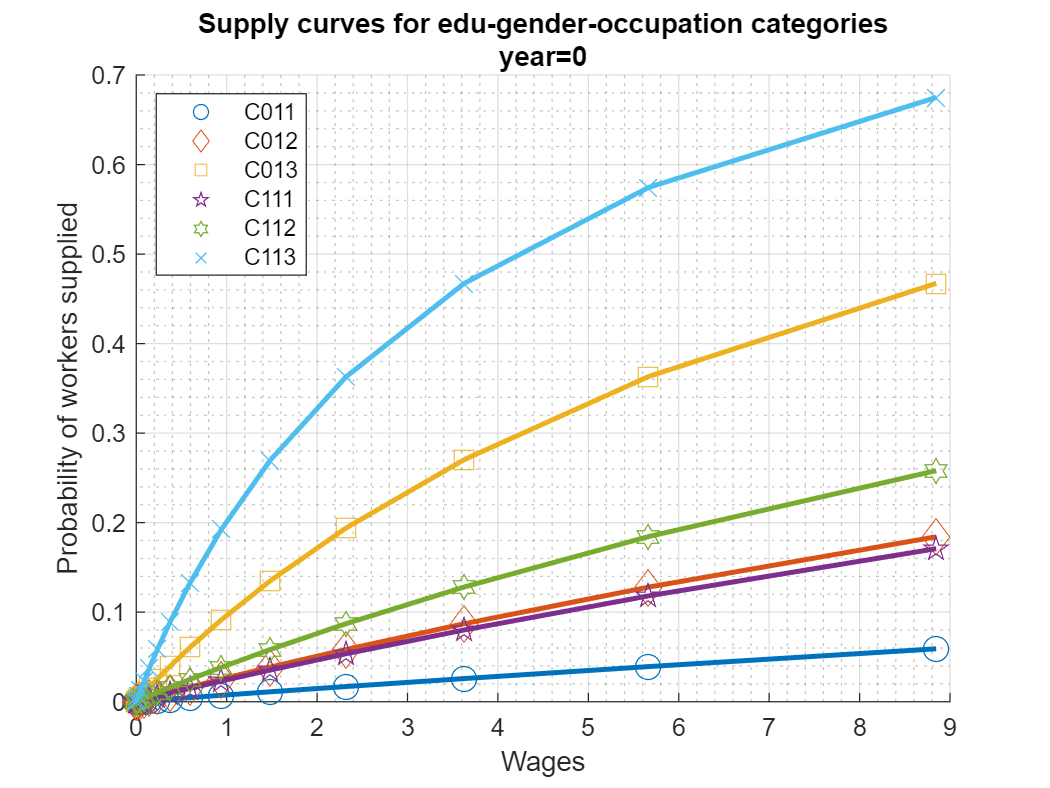
\includegraphics[width=5.20833in,height=\textheight]{img/bfwx_mlogit_images/figure_0.png}

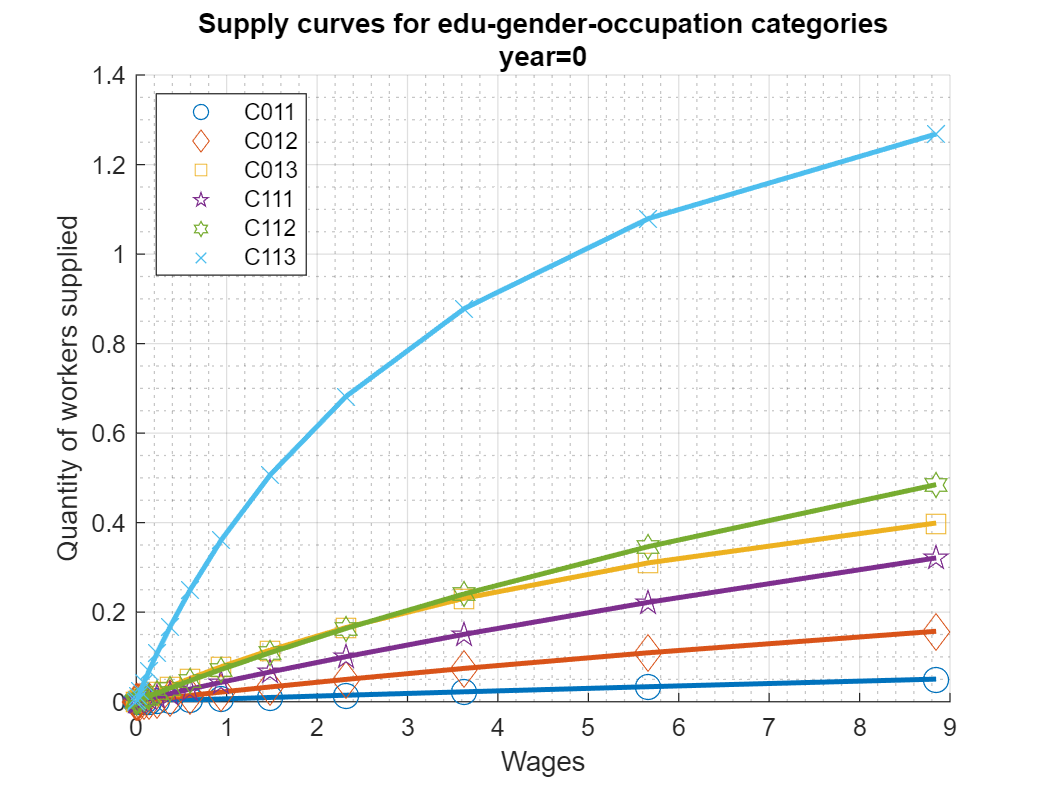
\includegraphics[width=5.20833in,height=\textheight]{img/bfwx_mlogit_images/figure_1.png}

\hypertarget{visualize-supply-curves-different-years}{%
\subsection{Visualize Supply Curves Different Years}\label{visualize-supply-curves-different-years}}

\begin{verbatim}
% 1. Print and Graph options
bl_verbose = false;
bl_graph = true;
ar_it_prob_or_quant = [1];

% 2. Get Parameters and data
bl_log_wage = true;
bl_verbose_nest = false;
% Get Parameters
mp_params = bfw_mp_param_esti(bl_log_wage);
mp_param_aux = bfw_mp_param_aux(bl_verbose_nest);
mp_params = [mp_params ; mp_param_aux];
% Get Data
mp_data = bfw_mp_data(bl_verbose_nest);
% Get Functions
mp_func = bfw_mp_func_supply(bl_log_wage, bl_verbose_nest);
% Get Controls
mp_controls = bfw_mp_control();

% 3. Data from which year, only integer year value allowed
% ar_it_data_year = [1989 1994 2000 2008 2014];
ar_it_data_year = [1989 2000 2014];
for it_data_year=ar_it_data_year

    % 4. Which categories to obtain data from, there are 12 possible
    % For non-college equilibrium, six wages, three female, three males
    % gen_occ = gender occupation
    for bl_skilled = [false true]
        if (bl_skilled)
            mt_st_gen_occ_categories = [...
                "C011", "C012", "C013"; ...
                "C111", "C112", "C113"];
        else
            mt_st_gen_occ_categories = [...
                "C001", "C002", "C003"; ...
                "C101", "C102", "C103"];
        end
        
        % 5. Array of wages, at most, since there are six nests, there are 12
        % prices possible. And there are 12 quantity supplies possible, coming
        % from four tyeps of workers, each supply 3 + home categories.
        mp_wages = containers.Map('KeyType', 'char', 'ValueType', 'any');
        % Obtain some equilibrium wage data as testing inputs
        mp_path = bfw_mp_path();
        spt_codem_data = mp_path('spt_codem_data');
        tb_data_pq = mp_data('tb_data_pq');
        tb_data_pq = tb_data_pq(:, ["year", "category", "numberWorkers", "meanWage"]);
        ar_st_gen_occ_categories = mt_st_gen_occ_categories(:)';
        for st_gen_occ=ar_st_gen_occ_categories
            tb_gen_occ_over_years = tb_data_pq(strcmp(tb_data_pq.category, st_gen_occ),:);
            fl_wage_one_year = tb_gen_occ_over_years(tb_gen_occ_over_years.year == (it_data_year), :);
            mp_wages(st_gen_occ) = fl_wage_one_year{1, "meanWage"};
        end

        % Print Wages
        % ff_container_map_display(mp_wages);

        % Get date offset
        params_group = values(mp_data, {'date_esti_offset'});
        [date_esti_offset] = params_group{:};

        % Run function
        [mp_fl_labor_occprbty,mp_fl_labor_supplied] = bfw_mlogit(...
            mp_params, mp_data, mp_func, mp_controls, ...
            mt_st_gen_occ_categories, it_data_year - date_esti_offset, mp_wages, ...
            bl_verbose, bl_graph, ...
            ar_it_prob_or_quant);
    end
end
\end{verbatim}

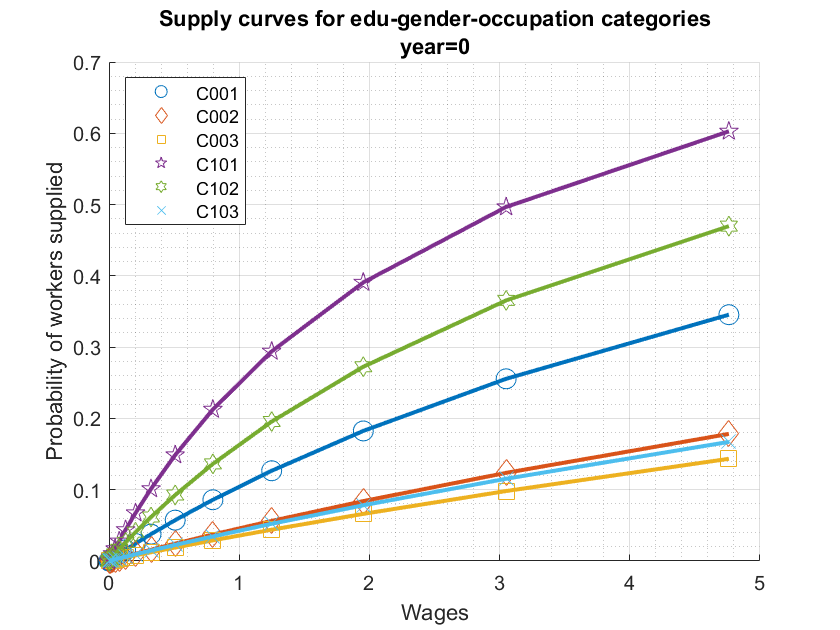
\includegraphics[width=5.20833in,height=\textheight]{img/bfwx_mlogit_images/figure_2.png}

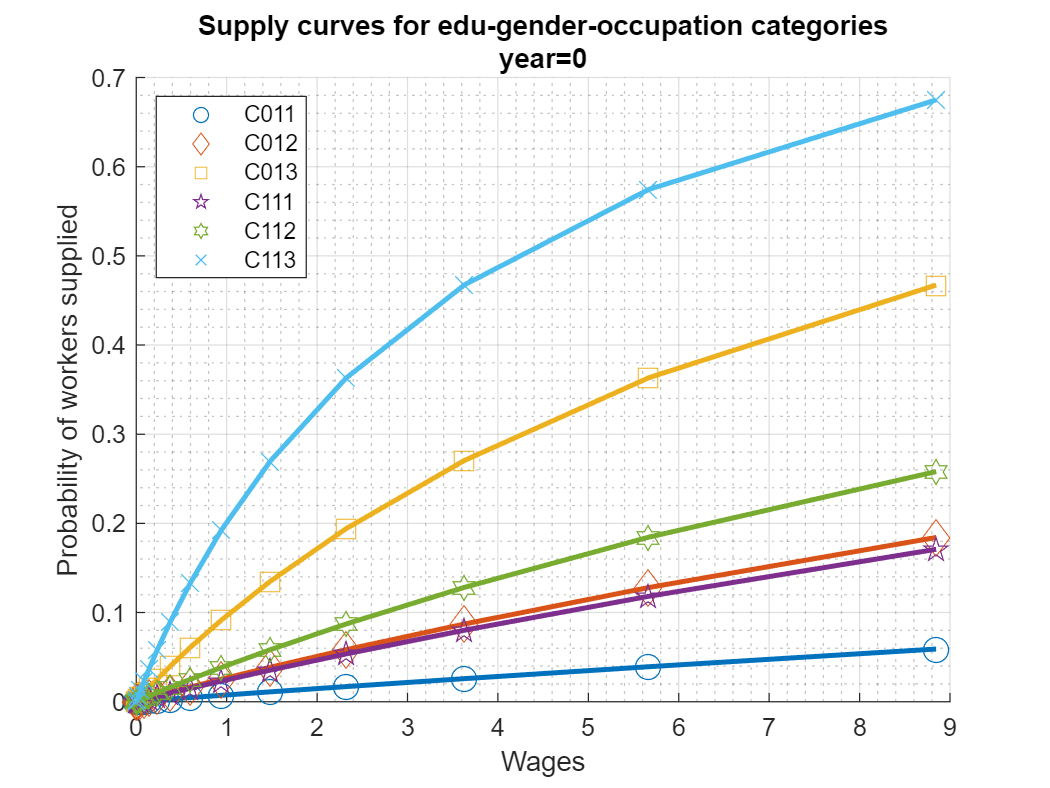
\includegraphics[width=5.20833in,height=\textheight]{img/bfwx_mlogit_images/figure_3.png}

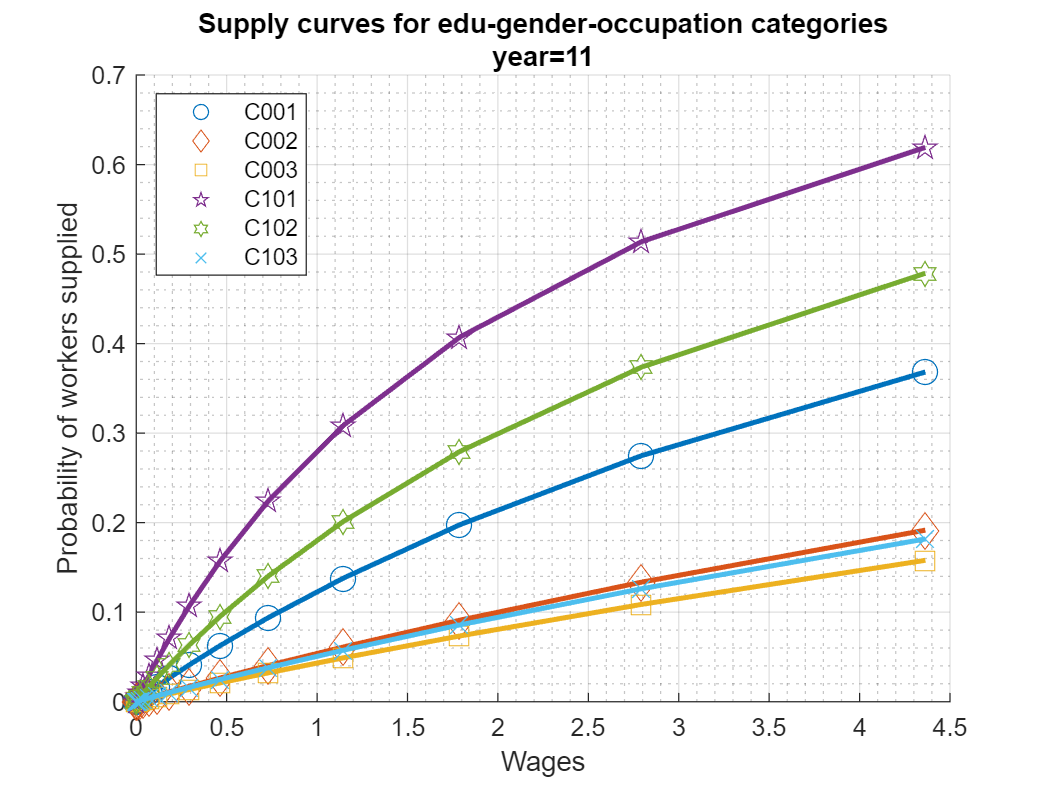
\includegraphics[width=5.20833in,height=\textheight]{img/bfwx_mlogit_images/figure_4.png}

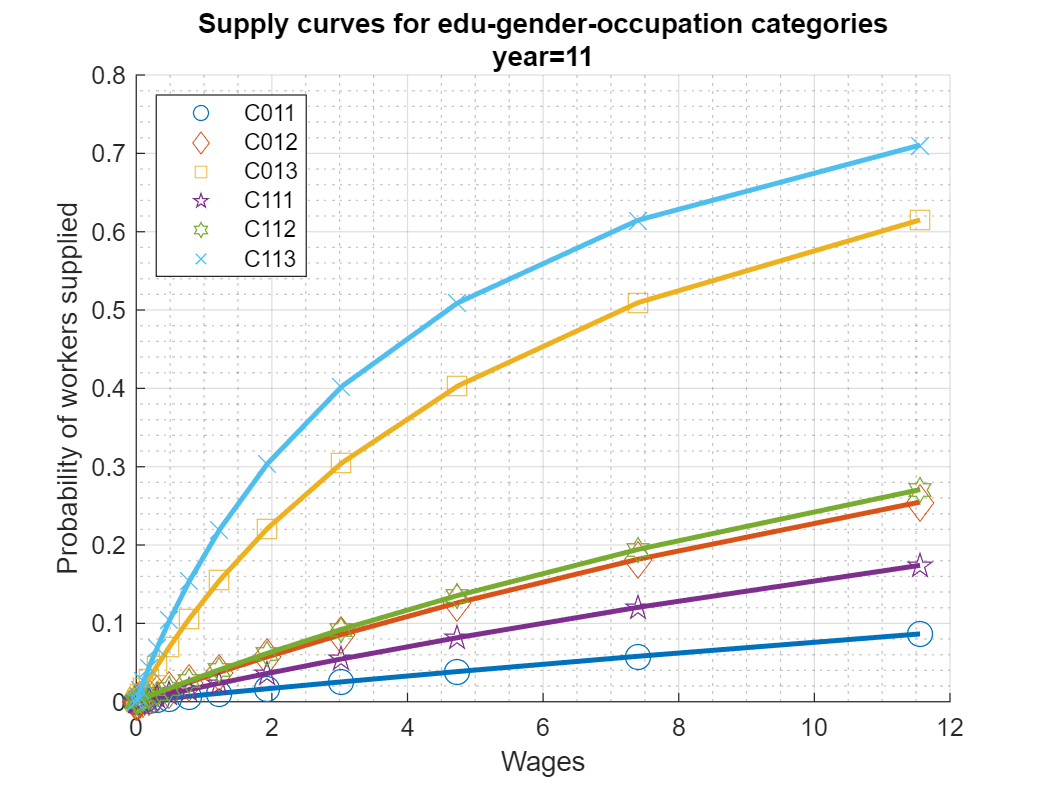
\includegraphics[width=5.20833in,height=\textheight]{img/bfwx_mlogit_images/figure_5.png}

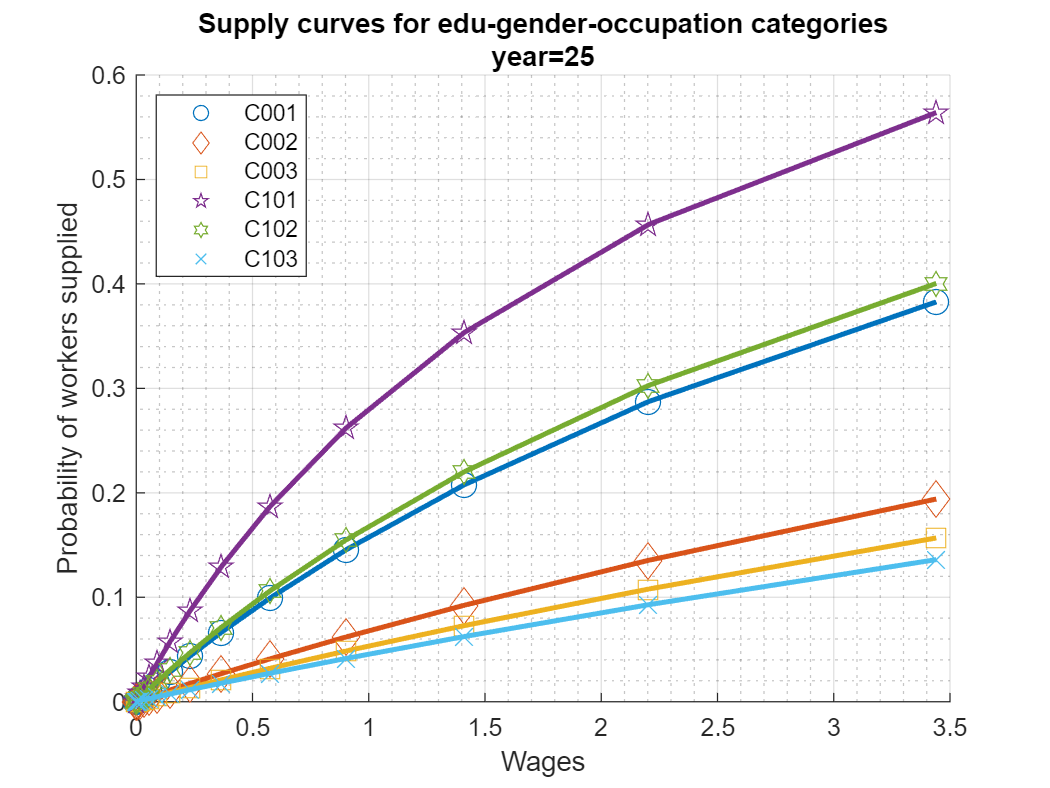
\includegraphics[width=5.20833in,height=\textheight]{img/bfwx_mlogit_images/figure_6.png}

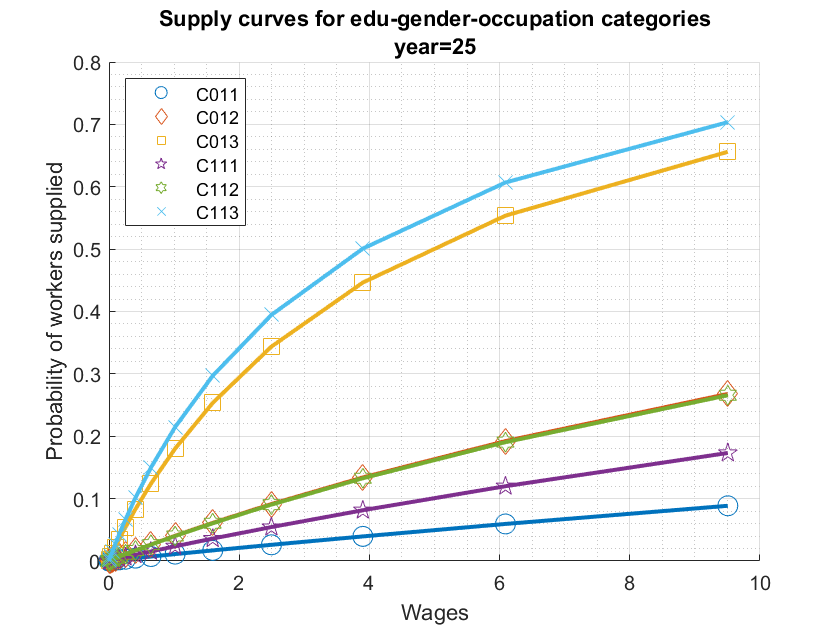
\includegraphics[width=5.20833in,height=\textheight]{img/bfwx_mlogit_images/figure_7.png}

\hypertarget{equilibrium-by-skill-nest-group}{%
\chapter{Equilibrium by Skill Nest Group}\label{equilibrium-by-skill-nest-group}}

\hypertarget{root-search-equilibrium-wage-equations-by-skill-group}{%
\section{Root Search Equilibrium Wage Equations By Skill Group}\label{root-search-equilibrium-wage-equations-by-skill-group}}

This is the example vignette for function: bfw\_solveequi\_kwfw from the
\href{https://fanwangecon.github.io/PrjLabEquiBFW/}{\textbf{PrjLabEquiBFW
Package}}\textbf{.}

\hypertarget{default-1}{%
\subsection{Default}\label{default-1}}

\begin{verbatim}
[mp_fl_labor_occprbty,mp_fl_labor_supplied] = bfw_solveequi_kwfw();

Completed BFW_SOLVEEQUI_KWFW;fl_potwrker_1=9.9687;fl_potwrker_2=12.5164;ar_fl_max_ratio_1=0.36095     0.25032     0.20764;ar_fl_max_ratio_2=0.34704     0.23222     0.16538
BFW_SOLVEEQUI_KWFW-initial-Q;category_key=;C001;sexrhs=;Female;occ=;Manual;wxox=3.5484;laborsupplied=2.2735
BFW_SOLVEEQUI_KWFW-initial-Q;category_key=;C002;sexrhs=;Female;occ=;Routine;wxox=4.9268;laborsupplied=1.6222
BFW_SOLVEEQUI_KWFW-initial-Q;category_key=;C003;sexrhs=;Female;occ=;Analytical;wxox=3.523;laborsupplied=1.341
BFW_SOLVEEQUI_KWFW-initial-Q;category_key=;C101;sexrhs=;Male;occ=;Manual;wxox=1.7656;laborsupplied=4.2925
BFW_SOLVEEQUI_KWFW-initial-Q;category_key=;C102;sexrhs=;Male;occ=;Routine;wxox=5.9065;laborsupplied=3.7644
BFW_SOLVEEQUI_KWFW-initial-Q;category_key=;C103;sexrhs=;Male;occ=;Analytical;wxox=2.222;laborsupplied=1.5416
Completed BFW_SOLVEEQUI_KWFW;fl_mse_excess=4.4821e-13;ar_w1_iter_endo=1.5779       1.819      3.7951;ar_w2_iter_hat=1.2165      1.8629       3.227;ar_w2_iter_gap=-6.527e-12 -1.9215e-07  8.4457e-07
----------------------------------------
xxxxxxxxxxxxxxxxxxxxxxxxxxxxxxxxxxxxxxxx
CONTAINER NAME: mp_wages Scalars
xxxxxxxxxxxxxxxxxxxxxxxxxxxxxxxxxxxxxxxx
            i    idx    value 
            _    ___    ______

    C001    1     1     1.2165
    C002    2     2     1.8629
    C003    3     3      3.227
    C101    4     4     1.5779
    C102    5     5      1.819
    C103    6     6     3.7951

----------------------------------------
xxxxxxxxxxxxxxxxxxxxxxxxxxxxxxxxxxxxxxxx
CONTAINER NAME: mp_fl_labor_demanded Scalars
xxxxxxxxxxxxxxxxxxxxxxxxxxxxxxxxxxxxxxxx
            i    idx    value 
            _    ___    ______

    C001    1     1     1.6514
    C002    2     2     1.0896
    C003    3     3     1.4662
    C101    4     4     4.3057
    C102    5     5     3.1524
    C103    6     6     1.9726

----------------------------------------
xxxxxxxxxxxxxxxxxxxxxxxxxxxxxxxxxxxxxxxx
CONTAINER NAME: mp_fl_labor_supplied Scalars
xxxxxxxxxxxxxxxxxxxxxxxxxxxxxxxxxxxxxxxx
            i    idx    value 
            _    ___    ______

    C001    1     1     1.6514
    C002    2     2     1.0896
    C003    3     3     1.4662
    C101    4     4     4.3057
    C102    5     5     3.1524
    C103    6     6     1.9726

----------------------------------------
xxxxxxxxxxxxxxxxxxxxxxxxxxxxxxxxxxxxxxxx
CONTAINER NAME: mp_fl_labor_occprbty Scalars
xxxxxxxxxxxxxxxxxxxxxxxxxxxxxxxxxxxxxxxx
            i    idx     value  
            _    ___    ________

    C001    1     1      0.13194
    C002    2     2     0.087055
    C003    3     3      0.11714
    C101    4     4      0.43193
    C102    5     5      0.31623
    C103    6     6      0.19788

----------------------------------------
xxxxxxxxxxxxxxxxxxxxxxxxxxxxxxxxxxxxxxxx
CONTAINER NAME: mp_fl_labor_excess_demand Scalars
xxxxxxxxxxxxxxxxxxxxxxxxxxxxxxxxxxxxxxxx
            i    idx       value   
            _    ___    ___________

    C001    1     1     -3.4607e-08
    C002    2     2     -2.3265e-07
    C003    3     3       6.268e-07
    C101    4     4     -2.6645e-15
    C102    5     5     -2.2204e-15
    C103    6     6     -2.2204e-16
\end{verbatim}

\hypertarget{vary-parameters-solve-equilibrium-quantitieswages-root-search}{%
\subsection{Vary Parameters, Solve Equilibrium Quantities/Wages, Root Search}\label{vary-parameters-solve-equilibrium-quantitieswages-root-search}}

\begin{verbatim}
% 2. Get Parameters and data
bl_log_wage = true;
bl_verbose_nest = false;

% Get Parameters
mp_params = bfw_mp_param_esti(bl_log_wage);
mp_param_aux = bfw_mp_param_aux(bl_verbose_nest);
mp_params = [mp_params ; mp_param_aux];

% Get Data
mp_data = bfw_mp_data(bl_verbose_nest);

% Get Functions
mp_func_demand = bfw_mp_func_demand(bl_verbose_nest);
mp_func_supply = bfw_mp_func_supply(bl_log_wage, bl_verbose_nest);
mp_func_equi = bfw_mp_func_equi(bl_verbose_nest);
mp_func = [mp_func_equi; mp_func_supply; mp_func_demand];

% Get Controls
mp_controls = bfw_mp_control();
mp_controls('bl_bfw_solveequi_kwfw_display') = false;
mp_controls('bl_bfw_solveequi_kwfw_display_verbose') = false;

st_exa_common_str = 'bfw_solveequi_kwfw()';
for it_example_inputs = [1,2,3,4]

    % Different testing scenariors
    if (it_example_inputs == 1)
        fl_rho_manual = 0.18;
        fl_rho_routine = 0.18;
        fl_rho_analytical = 0.18;

        fl_beta_1_manual = 1 - 0.26;
        fl_beta_1_routine = 1 - 0.30;
        fl_beta_1_analytical = 1 - 0.40;

        fl_Y_manual = 3.4084;
        fl_Y_routine = 2.3402;
        fl_Y_analytical = 1.7552;

        fl_w1o1_init = 2.315707;
        fl_w1o2_init = 3.217799;
        fl_w1o3_init = 4.329016;

        fl_w2o1_init = 1.942;
        fl_w2o2_init = 3.2247;
        fl_w2o3_init = 3.3738;

        it_data_year = 1989;
        fl_potwrker_1 = 9.9687;
        fl_potwrker_2 = 12.5164;
        bl_skilled = false;
        
        st_exa_string = "homogeneous rho at 0.18, unskilled";

    elseif (it_example_inputs == 2)
        fl_rho_manual = 0.64678;
        fl_rho_routine = 0.64678;
        fl_rho_analytical = 0.64678;

        fl_beta_1_manual = 0.63427;
        fl_beta_1_routine = 0.58738;
        fl_beta_1_analytical = 0.5784;

        fl_Y_manual = 3.2291;
        fl_Y_routine = 2.2223;
        fl_Y_analytical = 1.7487;

        fl_w1o1_init = 2.3157;
        fl_w1o2_init = 3.2178;
        fl_w1o3_init = 4.329;

        fl_w2o1_init = 1.942;
        fl_w2o2_init = 3.2247;
        fl_w2o3_init = 3.3738;

        it_data_year = 1989;
        fl_potwrker_1 = 9.9687;
        fl_potwrker_2 = 12.5164;

        bl_skilled = false;

        st_exa_string = "homogeneous rho at 0.64, unskilled";

    elseif (it_example_inputs == 3)
        fl_rho_manual = 0.34186;
        fl_rho_routine = 0.34186;
        fl_rho_analytical = 0.34186;

        fl_beta_1_manual = 0.63075;
        fl_beta_1_routine = 0.6326;
        fl_beta_1_analytical = 0.53894;

        fl_Y_manual = 5.5703;
        fl_Y_routine = 4.6673;
        fl_Y_analytical = 2.5644;

        fl_w1o1_init = 2.263;
        fl_w1o2_init = 2.5991;
        fl_w1o3_init = 3.6533;

        fl_w2o1_init = 1.7636;
        fl_w2o2_init = 2.4062;
        fl_w2o3_init = 2.8429;

        it_data_year = 2010;
        fl_potwrker_1 = 16.4952;
        fl_potwrker_2 = 19.4271;

        bl_skilled = false;

        st_exa_string = "homogeneous rho at 0.34, unskilled";

    elseif (it_example_inputs == 4)
        fl_rho_manual = 0.75002424;
        fl_rho_routine = 0.244249613;
        fl_rho_analytical = 0.244249613;

        fl_beta_1_manual = 0.703785173;
        fl_beta_1_routine = 0.687107264;
        fl_beta_1_analytical = 0.706254232;

        fl_Y_manual = 0.124479951;
        fl_Y_routine = 0.39857586;
        fl_Y_analytical = 1.388880655;

        fl_w1o1_init = 5.758649;
        fl_w1o2_init = 6.221019;
        fl_w1o3_init = 7.977073;

        fl_w2o1_init = 2.376239;
        fl_w2o2_init = 4.863073;
        fl_w2o3_init = 5.881686;

        it_data_year = 1996;
        fl_potwrker_1 = 16.4952;
        fl_potwrker_2 = 19.4271;

        bl_skilled = true;

        st_exa_string = "heter rho (0.75, 0.24, 0.24), skilled";

    end

    mp_params('fl_rho_manual') = fl_rho_manual;
    mp_params('fl_rho_routine') = fl_rho_routine;
    mp_params('fl_rho_analytical') = fl_rho_analytical;

    mp_params('fl_beta_1_manual') = fl_beta_1_manual;
    mp_params('fl_beta_1_routine') = fl_beta_1_routine;
    mp_params('fl_beta_1_analytical') = fl_beta_1_analytical;

    mp_params('fl_Y_manual') = fl_Y_manual;
    mp_params('fl_Y_routine') = fl_Y_routine;
    mp_params('fl_Y_analytical') = fl_Y_analytical;

    mp_data('fl_w1o1_init') = fl_w1o1_init;
    mp_data('fl_w1o2_init') = fl_w1o2_init;
    mp_data('fl_w1o3_init') = fl_w1o3_init;

    mp_data('fl_w2o1_init') = fl_w2o1_init;
    mp_data('fl_w2o2_init') = fl_w2o2_init;
    mp_data('fl_w2o3_init') = fl_w2o3_init;

    mp_data('fl_potwrker_1') = fl_potwrker_1;
    mp_data('fl_potwrker_2') = fl_potwrker_2;

    it_data_year = it_data_year - 1989;
    bl_checkminmax = true;
    it_solve_n1n2n3 = 3;
    [ar_w1_iter_endo, ar_w2_iter_hat, ar_w2_iter_gap, ...
        mp_wages, mp_fl_labor_demanded, mp_fl_labor_supplied, ...
        mp_fl_labor_occprbty, fl_mse_excess_demand, mp_fl_labor_excess_demand] = ...
        bfw_solveequi_kwfw(mp_params, mp_data, mp_func, mp_controls, ...
        it_solve_n1n2n3, it_data_year, bl_skilled, bl_checkminmax);

    disp('');
    disp('');
    disp('XXXXXXXXXXXXXXXXXXXXXXXXXXXXXXXXXXXXX');
    disp(['EXAMPLE ' num2str(it_example_inputs) ', ' st_exa_common_str ', ' char(st_exa_string)]);
    disp('XXXXXXXXXXXXXXXXXXXXXXXXXXXXXXXXXXXXX');
    ff_container_map_display(mp_wages);
    ff_container_map_display(mp_fl_labor_demanded);
    ff_container_map_display(mp_fl_labor_supplied);
    ff_container_map_display(mp_fl_labor_occprbty);
    ff_container_map_display(mp_fl_labor_excess_demand);

end

XXXXXXXXXXXXXXXXXXXXXXXXXXXXXXXXXXXXX
EXAMPLE 1, bfw_solveequi_kwfw(), homogeneous rho at 0.18, unskilled
XXXXXXXXXXXXXXXXXXXXXXXXXXXXXXXXXXXXX
----------------------------------------
xxxxxxxxxxxxxxxxxxxxxxxxxxxxxxxxxxxxxxxx
CONTAINER NAME: mp_wages Scalars
xxxxxxxxxxxxxxxxxxxxxxxxxxxxxxxxxxxxxxxx
            i    idx    value 
            _    ___    ______

    C001    1     1     1.2165
    C002    2     2     1.8629
    C003    3     3      3.227
    C101    4     4     1.5779
    C102    5     5      1.819
    C103    6     6     3.7951
----------------------------------------
xxxxxxxxxxxxxxxxxxxxxxxxxxxxxxxxxxxxxxxx
CONTAINER NAME: mp_fl_labor_demanded Scalars
xxxxxxxxxxxxxxxxxxxxxxxxxxxxxxxxxxxxxxxx
            i    idx    value 
            _    ___    ______

    C001    1     1     1.6514
    C002    2     2     1.0896
    C003    3     3     1.4662
    C101    4     4     4.3057
    C102    5     5     3.1524
    C103    6     6     1.9726
----------------------------------------
xxxxxxxxxxxxxxxxxxxxxxxxxxxxxxxxxxxxxxxx
CONTAINER NAME: mp_fl_labor_supplied Scalars
xxxxxxxxxxxxxxxxxxxxxxxxxxxxxxxxxxxxxxxx
            i    idx    value 
            _    ___    ______

    C001    1     1     1.6514
    C002    2     2     1.0896
    C003    3     3     1.4662
    C101    4     4     4.3057
    C102    5     5     3.1524
    C103    6     6     1.9726
----------------------------------------
xxxxxxxxxxxxxxxxxxxxxxxxxxxxxxxxxxxxxxxx
CONTAINER NAME: mp_fl_labor_occprbty Scalars
xxxxxxxxxxxxxxxxxxxxxxxxxxxxxxxxxxxxxxxx
            i    idx     value  
            _    ___    ________

    C001    1     1      0.13194
    C002    2     2     0.087055
    C003    3     3      0.11714
    C101    4     4      0.43193
    C102    5     5      0.31623
    C103    6     6      0.19788
----------------------------------------
xxxxxxxxxxxxxxxxxxxxxxxxxxxxxxxxxxxxxxxx
CONTAINER NAME: mp_fl_labor_excess_demand Scalars
xxxxxxxxxxxxxxxxxxxxxxxxxxxxxxxxxxxxxxxx
            i    idx       value   
            _    ___    ___________

    C001    1     1     -3.4607e-08
    C002    2     2     -2.3265e-07
    C003    3     3       6.268e-07
    C101    4     4     -2.6645e-15
    C102    5     5     -2.2204e-15
    C103    6     6     -2.2204e-16
XXXXXXXXXXXXXXXXXXXXXXXXXXXXXXXXXXXXX
EXAMPLE 2, bfw_solveequi_kwfw(), homogeneous rho at 0.64, unskilled
XXXXXXXXXXXXXXXXXXXXXXXXXXXXXXXXXXXXX
----------------------------------------
xxxxxxxxxxxxxxxxxxxxxxxxxxxxxxxxxxxxxxxx
CONTAINER NAME: mp_wages Scalars
xxxxxxxxxxxxxxxxxxxxxxxxxxxxxxxxxxxxxxxx
            i    idx    value 
            _    ___    ______

    C001    1     1     1.2481
    C002    2     2     1.8712
    C003    3     3     3.1468
    C101    4     4     1.5614
    C102    5     5     1.8288
    C103    6     6     3.8377
----------------------------------------
xxxxxxxxxxxxxxxxxxxxxxxxxxxxxxxxxxxxxxxx
CONTAINER NAME: mp_fl_labor_demanded Scalars
xxxxxxxxxxxxxxxxxxxxxxxxxxxxxxxxxxxxxxxx
            i    idx    value 
            _    ___    ______

    C001    1     1     1.6914
    C002    2     2     1.0934
    C003    3     3     1.4297
    C101    4     4     4.2646
    C102    5     5     3.1707
    C103    6     6     1.9952
----------------------------------------
xxxxxxxxxxxxxxxxxxxxxxxxxxxxxxxxxxxxxxxx
CONTAINER NAME: mp_fl_labor_supplied Scalars
xxxxxxxxxxxxxxxxxxxxxxxxxxxxxxxxxxxxxxxx
            i    idx    value 
            _    ___    ______

    C001    1     1     1.6914
    C002    2     2     1.0934
    C003    3     3     1.4297
    C101    4     4     4.2646
    C102    5     5     3.1707
    C103    6     6     1.9952
----------------------------------------
xxxxxxxxxxxxxxxxxxxxxxxxxxxxxxxxxxxxxxxx
CONTAINER NAME: mp_fl_labor_occprbty Scalars
xxxxxxxxxxxxxxxxxxxxxxxxxxxxxxxxxxxxxxxx
            i    idx     value  
            _    ___    ________

    C001    1     1      0.13513
    C002    2     2     0.087358
    C003    3     3      0.11423
    C101    4     4      0.42779
    C102    5     5      0.31807
    C103    6     6      0.20015
----------------------------------------
xxxxxxxxxxxxxxxxxxxxxxxxxxxxxxxxxxxxxxxx
CONTAINER NAME: mp_fl_labor_excess_demand Scalars
xxxxxxxxxxxxxxxxxxxxxxxxxxxxxxxxxxxxxxxx
            i    idx       value   
            _    ___    ___________

    C001    1     1      -9.373e-09
    C002    2     2     -1.9675e-07
    C003    3     3      3.6084e-07
    C101    4     4     -8.8818e-16
    C102    5     5      1.3323e-15
    C103    6     6     -2.2204e-16
XXXXXXXXXXXXXXXXXXXXXXXXXXXXXXXXXXXXX
EXAMPLE 3, bfw_solveequi_kwfw(), homogeneous rho at 0.34, unskilled
XXXXXXXXXXXXXXXXXXXXXXXXXXXXXXXXXXXXX
----------------------------------------
xxxxxxxxxxxxxxxxxxxxxxxxxxxxxxxxxxxxxxxx
CONTAINER NAME: mp_wages Scalars
xxxxxxxxxxxxxxxxxxxxxxxxxxxxxxxxxxxxxxxx
            i    idx    value 
            _    ___    ______

    C001    1     1     1.5675
    C002    2     2     2.5998
    C003    3     3     3.0763
    C101    4     4     1.9027
    C102    5     5     2.7234
    C103    6     6       3.72
----------------------------------------
xxxxxxxxxxxxxxxxxxxxxxxxxxxxxxxxxxxxxxxx
CONTAINER NAME: mp_fl_labor_demanded Scalars
xxxxxxxxxxxxxxxxxxxxxxxxxxxxxxxxxxxxxxxx
            i    idx    value 
            _    ___    ______

    C001    1     1     3.9729
    C002    2     2     2.8316
    C003    3     3     2.6363
    C101    4     4     6.6763
    C102    5     5     6.0249
    C103    6     6     2.5039
----------------------------------------
xxxxxxxxxxxxxxxxxxxxxxxxxxxxxxxxxxxxxxxx
CONTAINER NAME: mp_fl_labor_supplied Scalars
xxxxxxxxxxxxxxxxxxxxxxxxxxxxxxxxxxxxxxxx
            i    idx    value 
            _    ___    ______

    C001    1     1     3.9729
    C002    2     2     2.8316
    C003    3     3     2.6363
    C101    4     4     6.6763
    C102    5     5     6.0249
    C103    6     6     2.5039
----------------------------------------
xxxxxxxxxxxxxxxxxxxxxxxxxxxxxxxxxxxxxxxx
CONTAINER NAME: mp_fl_labor_occprbty Scalars
xxxxxxxxxxxxxxxxxxxxxxxxxxxxxxxxxxxxxxxx
            i    idx     value 
            _    ___    _______

    C001    1     1      0.2045
    C002    2     2     0.14575
    C003    3     3      0.1357
    C101    4     4     0.40474
    C102    5     5     0.36525
    C103    6     6      0.1518
----------------------------------------
xxxxxxxxxxxxxxxxxxxxxxxxxxxxxxxxxxxxxxxx
CONTAINER NAME: mp_fl_labor_excess_demand Scalars
xxxxxxxxxxxxxxxxxxxxxxxxxxxxxxxxxxxxxxxx
            i    idx       value   
            _    ___    ___________

    C001    1     1      8.8193e-08
    C002    2     2      6.1579e-07
    C003    3     3     -1.2231e-06
    C101    4     4     -3.5527e-15
    C102    5     5      1.7764e-15
    C103    6     6               0
XXXXXXXXXXXXXXXXXXXXXXXXXXXXXXXXXXXXX
EXAMPLE 4, bfw_solveequi_kwfw(), heter rho (0.75, 0.24, 0.24), skilled
XXXXXXXXXXXXXXXXXXXXXXXXXXXXXXXXXXXXX
----------------------------------------
xxxxxxxxxxxxxxxxxxxxxxxxxxxxxxxxxxxxxxxx
CONTAINER NAME: mp_wages Scalars
xxxxxxxxxxxxxxxxxxxxxxxxxxxxxxxxxxxxxxxx
            i    idx    value 
            _    ___    ______

    C011    1     1     2.2661
    C012    2     2     5.3853
    C013    3     3     6.7077
    C111    4     4     3.5562
    C112    5     5      6.838
    C113    6     6     9.4355
----------------------------------------
xxxxxxxxxxxxxxxxxxxxxxxxxxxxxxxxxxxxxxxx
CONTAINER NAME: mp_fl_labor_demanded Scalars
xxxxxxxxxxxxxxxxxxxxxxxxxxxxxxxxxxxxxxxx
            i    idx     value  
            _    ___    ________

    C011    1     1     0.032483
    C012    2     2      0.23898
    C013    3     3      0.83121
    C111    4     4       0.1707
    C112    5     5      0.49335
    C113    6     6       1.6895
----------------------------------------
xxxxxxxxxxxxxxxxxxxxxxxxxxxxxxxxxxxxxxxx
CONTAINER NAME: mp_fl_labor_supplied Scalars
xxxxxxxxxxxxxxxxxxxxxxxxxxxxxxxxxxxxxxxx
            i    idx     value  
            _    ___    ________

    C011    1     1     0.032483
    C012    2     2      0.23898
    C013    3     3      0.83121
    C111    4     4       0.1707
    C112    5     5      0.49335
    C113    6     6       1.6895
----------------------------------------
xxxxxxxxxxxxxxxxxxxxxxxxxxxxxxxxxxxxxxxx
CONTAINER NAME: mp_fl_labor_occprbty Scalars
xxxxxxxxxxxxxxxxxxxxxxxxxxxxxxxxxxxxxxxx
            i    idx     value  
            _    ___    ________

    C011    1     1     0.018322
    C012    2     2       0.1348
    C013    3     3      0.46886
    C111    4     4     0.068174
    C112    5     5      0.19703
    C113    6     6      0.67473
----------------------------------------
xxxxxxxxxxxxxxxxxxxxxxxxxxxxxxxxxxxxxxxx
CONTAINER NAME: mp_fl_labor_excess_demand Scalars
xxxxxxxxxxxxxxxxxxxxxxxxxxxxxxxxxxxxxxxx
            i    idx       value   
            _    ___    ___________

    C011    1     1     -1.8041e-09
    C012    2     2      5.6774e-08
    C013    3     3      8.1332e-08
    C111    4     4     -2.7756e-17
    C112    5     5      5.5511e-17
    C113    6     6      2.2204e-16
\end{verbatim}

\hypertarget{equilibrium-w-to-q-to-w-contraction-by-skill-group}{%
\section{Equilibrium W to Q to W Contraction By Skill Group}\label{equilibrium-w-to-q-to-w-contraction-by-skill-group}}

This is the example vignette for function: bfw\_solveequi\_w2q2w from the
\href{https://fanwangecon.github.io/PrjLabEquiBFW/}{\textbf{PrjLabEquiBFW
Package}}\textbf{.}

\hypertarget{default-2}{%
\subsection{Default}\label{default-2}}

\begin{verbatim}
[mp_fl_labor_occprbty,mp_fl_labor_supplied] = bfw_solveequi_w2q2w();

ITER:;it_speed_shifter_ctr=1;it_equi_wage_ctr=1;bl_continue=1;fl_ds_gap_mse=1.0294;fl_total_wage_change_mse=2.4494
    2.9507    2.8632    5.2962
    1.7458    2.4472    3.9586

    4.2925    3.7644    1.5416
    2.2735    1.6222    1.3410

    3.9933    2.9733    1.8551
    2.1150    1.2813    1.6136

ITER:;it_speed_shifter_ctr=1;it_equi_wage_ctr=2;bl_continue=1;fl_ds_gap_mse=0.62115;fl_total_wage_change_mse=1.2697
    2.0535    2.6792    5.8550
    1.4375    2.3313    4.0597

    4.9024    3.0389    1.6928
    2.1150    1.2813    1.6136

    4.1907    2.9908    1.7891
    1.8080    1.2610    1.7054

ITER:;it_speed_shifter_ctr=1;it_equi_wage_ctr=10;bl_continue=1;fl_ds_gap_mse=0.0075186;fl_total_wage_change_mse=0.025808
    1.5739    1.8511    3.9011
    1.2165    1.8810    3.2705

    4.3801    3.1280    1.9299
    1.6748    1.0915    1.4595

    4.3088    3.1446    1.9595
    1.6475    1.0973    1.4818

ITER:;it_speed_shifter_ctr=1;it_equi_wage_ctr=20;bl_continue=1;fl_ds_gap_mse=6.4007e-05;fl_total_wage_change_mse=0.0002943
    1.5762    1.8205    3.8023
    1.2159    1.8637    3.2298

    4.3126    3.1498    1.9685
    1.6528    1.0893    1.4649

    4.3065    3.1520    1.9717
    1.6505    1.0900    1.4673

ITER:;it_speed_shifter_ctr=1;it_equi_wage_ctr=30;bl_continue=1;fl_ds_gap_mse=6.0214e-07;fl_total_wage_change_mse=2.8652e-06
    1.5778    1.8191    3.7958
    1.2164    1.8629    3.2273

    4.3064    3.1522    1.9722
    1.6515    1.0896    1.4660

    4.3058    3.1524    1.9726
    1.6513    1.0897    1.4663

ITER:;it_speed_shifter_ctr=1;it_equi_wage_ctr=39;bl_continue=0;fl_ds_gap_mse=9.1058e-09;fl_total_wage_change_mse=4.3545e-08
    1.5780    1.8190    3.7950
    1.2165    1.8628    3.2270

    4.3057    3.1524    1.9727
    1.6514    1.0896    1.4662

    4.3057    3.1524    1.9727
    1.6514    1.0896    1.4662

----------------------------------------
xxxxxxxxxxxxxxxxxxxxxxxxxxxxxxxxxxxxxxxx
CONTAINER NAME: mp_wages Scalars
xxxxxxxxxxxxxxxxxxxxxxxxxxxxxxxxxxxxxxxx
            i    idx    value 
            _    ___    ______

    C001    1     1     1.2165
    C002    2     2     1.8628
    C003    3     3      3.227
    C101    4     4      1.578
    C102    5     5      1.819
    C103    6     6      3.795

----------------------------------------
xxxxxxxxxxxxxxxxxxxxxxxxxxxxxxxxxxxxxxxx
CONTAINER NAME: mp_fl_labor_supplied Scalars
xxxxxxxxxxxxxxxxxxxxxxxxxxxxxxxxxxxxxxxx
            i    idx    value 
            _    ___    ______

    C001    1     1     1.6514
    C002    2     2     1.0896
    C003    3     3     1.4662
    C101    4     4     4.3057
    C102    5     5     3.1524
    C103    6     6     1.9727

----------------------------------------
xxxxxxxxxxxxxxxxxxxxxxxxxxxxxxxxxxxxxxxx
CONTAINER NAME: mp_fl_labor_demanded Scalars
xxxxxxxxxxxxxxxxxxxxxxxxxxxxxxxxxxxxxxxx
            i    idx    value 
            _    ___    ______

    C001    1     1     1.6514
    C002    2     2     1.0896
    C003    3     3     1.4662
    C101    4     4     4.3057
    C102    5     5     3.1524
    C103    6     6     1.9727
\end{verbatim}

\hypertarget{vary-parameters-solve-equilibrium-quantities-wages-w-to-q-to-w-contraction}{%
\subsection{Vary Parameters, Solve Equilibrium Quantities Wages, W to Q to W Contraction}\label{vary-parameters-solve-equilibrium-quantities-wages-w-to-q-to-w-contraction}}

\begin{verbatim}
% 2. Get Parameters and data
bl_log_wage = true;
bl_verbose_nest = false;

% Get Parameters
mp_params = bfw_mp_param_esti(bl_log_wage);
mp_param_aux = bfw_mp_param_aux(bl_verbose_nest);
mp_params = [mp_params ; mp_param_aux];

% Get Data
mp_data = bfw_mp_data(bl_verbose_nest);

% Get Functions
mp_func_demand = bfw_mp_func_demand(bl_verbose_nest);
mp_func_supply = bfw_mp_func_supply(bl_log_wage, bl_verbose_nest);
mp_func_equi = bfw_mp_func_equi(bl_verbose_nest);
mp_func = [mp_func_equi; mp_func_supply; mp_func_demand];

% Get Controls
mp_controls = bfw_mp_control();
mp_controls('bl_bfw_solveequi_w2q2w_display') = false;
mp_controls('bl_bfw_solveequi_w2q2w_display_verbose') = false;

st_exa_common_str = 'bfw_solveequi_w2q2w()';
for it_example_inputs = [1,2,3,4]

    % Different testing scenariors
    if (it_example_inputs == 1)
        fl_rho_manual = 0.18;
        fl_rho_routine = 0.18;
        fl_rho_analytical = 0.18;

        fl_beta_1_manual = 1 - 0.26;
        fl_beta_1_routine = 1 - 0.30;
        fl_beta_1_analytical = 1 - 0.40;

        fl_Y_manual = 3.4084;
        fl_Y_routine = 2.3402;
        fl_Y_analytical = 1.7552;

        fl_w1o1_init = 2.315707;
        fl_w1o2_init = 3.217799;
        fl_w1o3_init = 4.329016;

        fl_w2o1_init = 1.942;
        fl_w2o2_init = 3.2247;
        fl_w2o3_init = 3.3738;

        it_data_year = 1989;
        fl_potwrker_1 = 9.9687;
        fl_potwrker_2 = 12.5164;
        bl_skilled = false;
        
        st_exa_string = "homogeneous rho at 0.18, unskilled";

    elseif (it_example_inputs == 2)
        fl_rho_manual = 0.64678;
        fl_rho_routine = 0.64678;
        fl_rho_analytical = 0.64678;

        fl_beta_1_manual = 0.63427;
        fl_beta_1_routine = 0.58738;
        fl_beta_1_analytical = 0.5784;

        fl_Y_manual = 3.2291;
        fl_Y_routine = 2.2223;
        fl_Y_analytical = 1.7487;

        fl_w1o1_init = 2.3157;
        fl_w1o2_init = 3.2178;
        fl_w1o3_init = 4.329;

        fl_w2o1_init = 1.942;
        fl_w2o2_init = 3.2247;
        fl_w2o3_init = 3.3738;

        it_data_year = 1989;
        fl_potwrker_1 = 9.9687;
        fl_potwrker_2 = 12.5164;

        bl_skilled = false;

        st_exa_string = "homogeneous rho at 0.64, unskilled";

    elseif (it_example_inputs == 3)
        fl_rho_manual = 0.34186;
        fl_rho_routine = 0.34186;
        fl_rho_analytical = 0.34186;

        fl_beta_1_manual = 0.63075;
        fl_beta_1_routine = 0.6326;
        fl_beta_1_analytical = 0.53894;

        fl_Y_manual = 5.5703;
        fl_Y_routine = 4.6673;
        fl_Y_analytical = 2.5644;

        fl_w1o1_init = 2.263;
        fl_w1o2_init = 2.5991;
        fl_w1o3_init = 3.6533;

        fl_w2o1_init = 1.7636;
        fl_w2o2_init = 2.4062;
        fl_w2o3_init = 2.8429;

        it_data_year = 2010;
        fl_potwrker_1 = 16.4952;
        fl_potwrker_2 = 19.4271;

        bl_skilled = false;

        st_exa_string = "homogeneous rho at 0.34, unskilled";

    elseif (it_example_inputs == 4)
        fl_rho_manual = 0.75002424;
        fl_rho_routine = 0.244249613;
        fl_rho_analytical = 0.244249613;

        fl_beta_1_manual = 0.703785173;
        fl_beta_1_routine = 0.687107264;
        fl_beta_1_analytical = 0.706254232;

        fl_Y_manual = 0.124479951;
        fl_Y_routine = 0.39857586;
        fl_Y_analytical = 1.388880655;

        fl_w1o1_init = 5.758649;
        fl_w1o2_init = 6.221019;
        fl_w1o3_init = 7.977073;

        fl_w2o1_init = 2.376239;
        fl_w2o2_init = 4.863073;
        fl_w2o3_init = 5.881686;

        it_data_year = 1996;
        fl_potwrker_1 = 16.4952;
        fl_potwrker_2 = 19.4271;

        bl_skilled = true;

        st_exa_string = "heter rho (0.75, 0.24, 0.24), skilled";

    end

    mp_params('fl_rho_manual') = fl_rho_manual;
    mp_params('fl_rho_routine') = fl_rho_routine;
    mp_params('fl_rho_analytical') = fl_rho_analytical;

    mp_params('fl_beta_1_manual') = fl_beta_1_manual;
    mp_params('fl_beta_1_routine') = fl_beta_1_routine;
    mp_params('fl_beta_1_analytical') = fl_beta_1_analytical;

    mp_params('fl_Y_manual') = fl_Y_manual;
    mp_params('fl_Y_routine') = fl_Y_routine;
    mp_params('fl_Y_analytical') = fl_Y_analytical;

    mp_data('fl_w1o1_init') = fl_w1o1_init;
    mp_data('fl_w1o2_init') = fl_w1o2_init;
    mp_data('fl_w1o3_init') = fl_w1o3_init;

    mp_data('fl_w2o1_init') = fl_w2o1_init;
    mp_data('fl_w2o2_init') = fl_w2o2_init;
    mp_data('fl_w2o3_init') = fl_w2o3_init;

    mp_data('fl_potwrker_1') = fl_potwrker_1;
    mp_data('fl_potwrker_2') = fl_potwrker_2;

    it_data_year = it_data_year - 1989;
    bl_checkminmax = true;
    it_solve_n1n2n3 = 3;
    [~, ~, ~, ~, ~, ~, ~, ~, ~, ...
        mp_wages, mp_fl_labor_demanded, mp_fl_labor_supplied, ...
        mp_fl_labor_occprbty] = ...
        bfw_solveequi_w2q2w(mp_params, mp_data, mp_func, mp_controls, ...
        it_solve_n1n2n3, it_data_year, bl_skilled, bl_checkminmax);

    disp('');
    disp('');
    disp('XXXXXXXXXXXXXXXXXXXXXXXXXXXXXXXXXXXXX');
    disp(['EXAMPLE ' num2str(it_example_inputs) ', ' st_exa_common_str ', ' char(st_exa_string)]);
    disp('XXXXXXXXXXXXXXXXXXXXXXXXXXXXXXXXXXXXX');
    ff_container_map_display(mp_wages);
    ff_container_map_display(mp_fl_labor_demanded);
    ff_container_map_display(mp_fl_labor_supplied);
    ff_container_map_display(mp_fl_labor_occprbty);

end

XXXXXXXXXXXXXXXXXXXXXXXXXXXXXXXXXXXXX
EXAMPLE 1, bfw_solveequi_w2q2w(), homogeneous rho at 0.18, unskilled
XXXXXXXXXXXXXXXXXXXXXXXXXXXXXXXXXXXXX
----------------------------------------
xxxxxxxxxxxxxxxxxxxxxxxxxxxxxxxxxxxxxxxx
CONTAINER NAME: mp_wages Scalars
xxxxxxxxxxxxxxxxxxxxxxxxxxxxxxxxxxxxxxxx
            i    idx    value 
            _    ___    ______

    C001    1     1     1.2165
    C002    2     2     1.8628
    C003    3     3      3.227
    C101    4     4      1.578
    C102    5     5      1.819
    C103    6     6      3.795
----------------------------------------
xxxxxxxxxxxxxxxxxxxxxxxxxxxxxxxxxxxxxxxx
CONTAINER NAME: mp_fl_labor_demanded Scalars
xxxxxxxxxxxxxxxxxxxxxxxxxxxxxxxxxxxxxxxx
            i    idx    value 
            _    ___    ______

    C001    1     1     1.6514
    C002    2     2     1.0896
    C003    3     3     1.4662
    C101    4     4     4.3057
    C102    5     5     3.1524
    C103    6     6     1.9727
----------------------------------------
xxxxxxxxxxxxxxxxxxxxxxxxxxxxxxxxxxxxxxxx
CONTAINER NAME: mp_fl_labor_supplied Scalars
xxxxxxxxxxxxxxxxxxxxxxxxxxxxxxxxxxxxxxxx
            i    idx    value 
            _    ___    ______

    C001    1     1     1.6514
    C002    2     2     1.0896
    C003    3     3     1.4662
    C101    4     4     4.3057
    C102    5     5     3.1524
    C103    6     6     1.9727
----------------------------------------
xxxxxxxxxxxxxxxxxxxxxxxxxxxxxxxxxxxxxxxx
CONTAINER NAME: mp_fl_labor_occprbty Scalars
xxxxxxxxxxxxxxxxxxxxxxxxxxxxxxxxxxxxxxxx
            i    idx     value  
            _    ___    ________

    C001    1     1      0.13194
    C002    2     2     0.087055
    C003    3     3      0.11714
    C101    4     4      0.43193
    C102    5     5      0.31623
    C103    6     6      0.19788
XXXXXXXXXXXXXXXXXXXXXXXXXXXXXXXXXXXXX
EXAMPLE 2, bfw_solveequi_w2q2w(), homogeneous rho at 0.64, unskilled
XXXXXXXXXXXXXXXXXXXXXXXXXXXXXXXXXXXXX
----------------------------------------
xxxxxxxxxxxxxxxxxxxxxxxxxxxxxxxxxxxxxxxx
CONTAINER NAME: mp_wages Scalars
xxxxxxxxxxxxxxxxxxxxxxxxxxxxxxxxxxxxxxxx
            i    idx    value 
            _    ___    ______

    C001    1     1     1.2482
    C002    2     2     1.8713
    C003    3     3     3.1469
    C101    4     4     1.5614
    C102    5     5     1.8289
    C103    6     6     3.8378
----------------------------------------
xxxxxxxxxxxxxxxxxxxxxxxxxxxxxxxxxxxxxxxx
CONTAINER NAME: mp_fl_labor_demanded Scalars
xxxxxxxxxxxxxxxxxxxxxxxxxxxxxxxxxxxxxxxx
            i    idx    value 
            _    ___    ______

    C001    1     1     1.6914
    C002    2     2     1.0934
    C003    3     3     1.4297
    C101    4     4     4.2646
    C102    5     5     3.1708
    C103    6     6     1.9952
----------------------------------------
xxxxxxxxxxxxxxxxxxxxxxxxxxxxxxxxxxxxxxxx
CONTAINER NAME: mp_fl_labor_supplied Scalars
xxxxxxxxxxxxxxxxxxxxxxxxxxxxxxxxxxxxxxxx
            i    idx    value 
            _    ___    ______

    C001    1     1     1.6914
    C002    2     2     1.0934
    C003    3     3     1.4297
    C101    4     4     4.2645
    C102    5     5     3.1707
    C103    6     6     1.9952
----------------------------------------
xxxxxxxxxxxxxxxxxxxxxxxxxxxxxxxxxxxxxxxx
CONTAINER NAME: mp_fl_labor_occprbty Scalars
xxxxxxxxxxxxxxxxxxxxxxxxxxxxxxxxxxxxxxxx
            i    idx     value  
            _    ___    ________

    C001    1     1      0.13514
    C002    2     2     0.087359
    C003    3     3      0.11423
    C101    4     4      0.42779
    C102    5     5      0.31807
    C103    6     6      0.20014
XXXXXXXXXXXXXXXXXXXXXXXXXXXXXXXXXXXXX
EXAMPLE 3, bfw_solveequi_w2q2w(), homogeneous rho at 0.34, unskilled
XXXXXXXXXXXXXXXXXXXXXXXXXXXXXXXXXXXXX
----------------------------------------
xxxxxxxxxxxxxxxxxxxxxxxxxxxxxxxxxxxxxxxx
CONTAINER NAME: mp_wages Scalars
xxxxxxxxxxxxxxxxxxxxxxxxxxxxxxxxxxxxxxxx
            i    idx    value 
            _    ___    ______

    C001    1     1     1.5675
    C002    2     2     2.5998
    C003    3     3     3.0763
    C101    4     4     1.9027
    C102    5     5     2.7234
    C103    6     6       3.72
----------------------------------------
xxxxxxxxxxxxxxxxxxxxxxxxxxxxxxxxxxxxxxxx
CONTAINER NAME: mp_fl_labor_demanded Scalars
xxxxxxxxxxxxxxxxxxxxxxxxxxxxxxxxxxxxxxxx
            i    idx    value 
            _    ___    ______

    C001    1     1     3.9729
    C002    2     2     2.8316
    C003    3     3     2.6364
    C101    4     4     6.6763
    C102    5     5     6.0249
    C103    6     6     2.5039
----------------------------------------
xxxxxxxxxxxxxxxxxxxxxxxxxxxxxxxxxxxxxxxx
CONTAINER NAME: mp_fl_labor_supplied Scalars
xxxxxxxxxxxxxxxxxxxxxxxxxxxxxxxxxxxxxxxx
            i    idx    value 
            _    ___    ______

    C001    1     1     3.9729
    C002    2     2     2.8316
    C003    3     3     2.6363
    C101    4     4     6.6763
    C102    5     5     6.0249
    C103    6     6     2.5039
----------------------------------------
xxxxxxxxxxxxxxxxxxxxxxxxxxxxxxxxxxxxxxxx
CONTAINER NAME: mp_fl_labor_occprbty Scalars
xxxxxxxxxxxxxxxxxxxxxxxxxxxxxxxxxxxxxxxx
            i    idx     value 
            _    ___    _______

    C001    1     1      0.2045
    C002    2     2     0.14576
    C003    3     3      0.1357
    C101    4     4     0.40474
    C102    5     5     0.36525
    C103    6     6      0.1518
XXXXXXXXXXXXXXXXXXXXXXXXXXXXXXXXXXXXX
EXAMPLE 4, bfw_solveequi_w2q2w(), heter rho (0.75, 0.24, 0.24), skilled
XXXXXXXXXXXXXXXXXXXXXXXXXXXXXXXXXXXXX
----------------------------------------
xxxxxxxxxxxxxxxxxxxxxxxxxxxxxxxxxxxxxxxx
CONTAINER NAME: mp_wages Scalars
xxxxxxxxxxxxxxxxxxxxxxxxxxxxxxxxxxxxxxxx
            i    idx    value 
            _    ___    ______

    C011    1     1     2.2661
    C012    2     2     5.3851
    C013    3     3     6.7078
    C111    4     4     3.5562
    C112    5     5     6.8374
    C113    6     6     9.4358
----------------------------------------
xxxxxxxxxxxxxxxxxxxxxxxxxxxxxxxxxxxxxxxx
CONTAINER NAME: mp_fl_labor_demanded Scalars
xxxxxxxxxxxxxxxxxxxxxxxxxxxxxxxxxxxxxxxx
            i    idx     value  
            _    ___    ________

    C011    1     1     0.032483
    C012    2     2      0.23899
    C013    3     3       0.8312
    C111    4     4       0.1707
    C112    5     5      0.49341
    C113    6     6       1.6894
----------------------------------------
xxxxxxxxxxxxxxxxxxxxxxxxxxxxxxxxxxxxxxxx
CONTAINER NAME: mp_fl_labor_supplied Scalars
xxxxxxxxxxxxxxxxxxxxxxxxxxxxxxxxxxxxxxxx
            i    idx     value  
            _    ___    ________

    C011    1     1     0.032483
    C012    2     2      0.23897
    C013    3     3      0.83122
    C111    4     4       0.1707
    C112    5     5      0.49336
    C113    6     6       1.6895
----------------------------------------
xxxxxxxxxxxxxxxxxxxxxxxxxxxxxxxxxxxxxxxx
CONTAINER NAME: mp_fl_labor_occprbty Scalars
xxxxxxxxxxxxxxxxxxxxxxxxxxxxxxxxxxxxxxxx
            i    idx     value  
            _    ___    ________

    C011    1     1     0.018322
    C012    2     2      0.13479
    C013    3     3      0.46886
    C111    4     4     0.068174
    C112    5     5      0.19704
    C113    6     6      0.67473
\end{verbatim}

\hypertarget{appendix-appendix}{%
\appendix}


\hypertarget{index-and-code-links}{%
\chapter{Index and Code Links}\label{index-and-code-links}}

\hypertarget{introduction-links}{%
\section{Introduction links}\label{introduction-links}}

\begin{enumerate}
\def\labelenumi{\arabic{enumi}.}
\tightlist
\item
  \href{https://fanwangecon.github.io/PrjLabEquiBFW/PrjLabEquiBFW/doc/intro/htmlpdfm/bfwx_intro.html}{The Labor Demand and Supply Problem}: \href{https://github.com/FanWangEcon/PrjLabEquiBFW/blob/master/PrjLabEquiBFW/doc/intro/bfwx_intro.mlx}{\textbf{mlx}} \textbar{} \href{https://github.com/FanWangEcon/PrjLabEquiBFW/blob/master/PrjLabEquiBFW/doc/intro/htmlpdfm/bfwx_intro.m}{\textbf{m}} \textbar{} \href{https://github.com/FanWangEcon/PrjLabEquiBFW/blob/master/PrjLabEquiBFW/doc/intro/htmlpdfm/bfwx_intro.pdf}{\textbf{pdf}} \textbar{} \href{https://fanwangecon.github.io/PrjLabEquiBFW/PrjLabEquiBFW/doc/intro/htmlpdfm/bfwx_intro.html}{\textbf{html}}

  \begin{itemize}
  \tightlist
  \item
    The Labor Demand and Supply Problem
  \end{itemize}
\end{enumerate}

\hypertarget{core-functions-links}{%
\section{Core Functions links}\label{core-functions-links}}

\begin{enumerate}
\def\labelenumi{\arabic{enumi}.}
\tightlist
\item
  \href{https://fanwangecon.github.io/PrjLabEquiBFW/PrjLabEquiBFW/doc/func/htmlpdfm/bfwx_mp_func_demand.html}{CES Demand Core Functions}: \href{https://github.com/FanWangEcon/PrjLabEquiBFW/blob/master/PrjLabEquiBFW/doc/func/bfwx_mp_func_demand.mlx}{\textbf{mlx}} \textbar{} \href{https://github.com/FanWangEcon/PrjLabEquiBFW/blob/master/PrjLabEquiBFW/doc/func/htmlpdfm/bfwx_mp_func_demand.m}{\textbf{m}} \textbar{} \href{https://github.com/FanWangEcon/PrjLabEquiBFW/blob/master/PrjLabEquiBFW/doc/func/htmlpdfm/bfwx_mp_func_demand.pdf}{\textbf{pdf}} \textbar{} \href{https://fanwangecon.github.io/PrjLabEquiBFW/PrjLabEquiBFW/doc/func/htmlpdfm/bfwx_mp_func_demand.html}{\textbf{html}}

  \begin{itemize}
  \tightlist
  \item
    This function generates a container map with key CES demand-side equation for a particular sub-nest.
  \item
    \textbf{PrjLabEquiBFW}: \emph{\href{https://github.com/FanWangEcon/PrjLabEquiBFW/blob/main/PrjLabEquiBFW/func/bfw_mp_func_demand.m}{bfw\_mp\_func\_demand()}}
  \end{itemize}
\item
  \href{https://fanwangecon.github.io/PrjLabEquiBFW/PrjLabEquiBFW/doc/func/htmlpdfm/bfwx_mp_func_supply.html}{Multinomial Logit Core Functions}: \href{https://github.com/FanWangEcon/PrjLabEquiBFW/blob/master/PrjLabEquiBFW/doc/func/bfwx_mp_func_supply.mlx}{\textbf{mlx}} \textbar{} \href{https://github.com/FanWangEcon/PrjLabEquiBFW/blob/master/PrjLabEquiBFW/doc/func/htmlpdfm/bfwx_mp_func_supply.m}{\textbf{m}} \textbar{} \href{https://github.com/FanWangEcon/PrjLabEquiBFW/blob/master/PrjLabEquiBFW/doc/func/htmlpdfm/bfwx_mp_func_supply.pdf}{\textbf{pdf}} \textbar{} \href{https://fanwangecon.github.io/PrjLabEquiBFW/PrjLabEquiBFW/doc/func/htmlpdfm/bfwx_mp_func_supply.html}{\textbf{html}}

  \begin{itemize}
  \tightlist
  \item
    This function generates a container map with key multinomial logit supply-side equations.
  \item
    \textbf{PrjLabEquiBFW}: \emph{\href{https://github.com/FanWangEcon/PrjLabEquiBFW/blob/main/PrjLabEquiBFW/func/bfw_mp_func_supply.m}{bfw\_mp\_func\_supply()}}
  \end{itemize}
\item
  \href{https://fanwangecon.github.io/PrjLabEquiBFW/PrjLabEquiBFW/doc/func/htmlpdfm/bfwx_mp_func_equi.html}{Equilibrium Core Functions}: \href{https://github.com/FanWangEcon/PrjLabEquiBFW/blob/master/PrjLabEquiBFW/doc/func/bfwx_mp_func_equi.mlx}{\textbf{mlx}} \textbar{} \href{https://github.com/FanWangEcon/PrjLabEquiBFW/blob/master/PrjLabEquiBFW/doc/func/htmlpdfm/bfwx_mp_func_equi.m}{\textbf{m}} \textbar{} \href{https://github.com/FanWangEcon/PrjLabEquiBFW/blob/master/PrjLabEquiBFW/doc/func/htmlpdfm/bfwx_mp_func_equi.pdf}{\textbf{pdf}} \textbar{} \href{https://fanwangecon.github.io/PrjLabEquiBFW/PrjLabEquiBFW/doc/func/htmlpdfm/bfwx_mp_func_equi.html}{\textbf{html}}

  \begin{itemize}
  \tightlist
  \item
    This function generates a container map with key equilibrium equations.
  \item
    \textbf{PrjLabEquiBFW}: \emph{\href{https://github.com/FanWangEcon/PrjLabEquiBFW/blob/main/PrjLabEquiBFW/func/bfw_mp_func_equi.m}{bfw\_mp\_func\_equi()}}
  \end{itemize}
\end{enumerate}

\hypertarget{parameters-links}{%
\section{Parameters links}\label{parameters-links}}

\begin{enumerate}
\def\labelenumi{\arabic{enumi}.}
\tightlist
\item
  \href{https://fanwangecon.github.io/PrjLabEquiBFW/PrjLabEquiBFW/doc/params/htmlpdfm/bfwx_mp_path.html}{bfwx\_mp\_path}: \href{https://github.com/FanWangEcon/PrjLabEquiBFW/blob/master/PrjLabEquiBFW/doc/params/bfwx_mp_path.mlx}{\textbf{mlx}} \textbar{} \href{https://github.com/FanWangEcon/PrjLabEquiBFW/blob/master/PrjLabEquiBFW/doc/params/htmlpdfm/bfwx_mp_path.m}{\textbf{m}} \textbar{} \href{https://github.com/FanWangEcon/PrjLabEquiBFW/blob/master/PrjLabEquiBFW/doc/params/htmlpdfm/bfwx_mp_path.pdf}{\textbf{pdf}} \textbar{} \href{https://fanwangecon.github.io/PrjLabEquiBFW/PrjLabEquiBFW/doc/params/htmlpdfm/bfwx_mp_path.html}{\textbf{html}}

  \begin{itemize}
  \tightlist
  \item
    bfw\_mp\_path
  \item
    \textbf{PrjLabEquiBFW}: \emph{\href{https://github.com/FanWangEcon/PrjLabEquiBFW/blob/main/PrjLabEquiBFW/paramsdata/bfw_mp_path.m}{bfw\_mp\_path()}}
  \end{itemize}
\item
  \href{https://fanwangecon.github.io/PrjLabEquiBFW/PrjLabEquiBFW/doc/params/htmlpdfm/bfwx_mp_control.html}{bfwx\_mp\_control}: \href{https://github.com/FanWangEcon/PrjLabEquiBFW/blob/master/PrjLabEquiBFW/doc/params/bfwx_mp_control.mlx}{\textbf{mlx}} \textbar{} \href{https://github.com/FanWangEcon/PrjLabEquiBFW/blob/master/PrjLabEquiBFW/doc/params/htmlpdfm/bfwx_mp_control.m}{\textbf{m}} \textbar{} \href{https://github.com/FanWangEcon/PrjLabEquiBFW/blob/master/PrjLabEquiBFW/doc/params/htmlpdfm/bfwx_mp_control.pdf}{\textbf{pdf}} \textbar{} \href{https://fanwangecon.github.io/PrjLabEquiBFW/PrjLabEquiBFW/doc/params/htmlpdfm/bfwx_mp_control.html}{\textbf{html}}

  \begin{itemize}
  \tightlist
  \item
    bfw\_mp\_control
  \item
    \textbf{PrjLabEquiBFW}: \emph{\href{https://github.com/FanWangEcon/PrjLabEquiBFW/blob/main/PrjLabEquiBFW/paramsdata/bfw_mp_control.m}{bfw\_mp\_control()}}
  \end{itemize}
\item
  \href{https://fanwangecon.github.io/PrjLabEquiBFW/PrjLabEquiBFW/doc/params/htmlpdfm/bfwx_mp_param_esti.html}{bfw\_mp\_param\_esti}: \href{https://github.com/FanWangEcon/PrjLabEquiBFW/blob/master/PrjLabEquiBFW/doc/params/bfwx_mp_param_esti.mlx}{\textbf{mlx}} \textbar{} \href{https://github.com/FanWangEcon/PrjLabEquiBFW/blob/master/PrjLabEquiBFW/doc/params/htmlpdfm/bfwx_mp_param_esti.m}{\textbf{m}} \textbar{} \href{https://github.com/FanWangEcon/PrjLabEquiBFW/blob/master/PrjLabEquiBFW/doc/params/htmlpdfm/bfwx_mp_param_esti.pdf}{\textbf{pdf}} \textbar{} \href{https://fanwangecon.github.io/PrjLabEquiBFW/PrjLabEquiBFW/doc/params/htmlpdfm/bfwx_mp_param_esti.html}{\textbf{html}}

  \begin{itemize}
  \tightlist
  \item
    bfw\_mp\_param\_esti
  \item
    \textbf{PrjLabEquiBFW}: \emph{\href{https://github.com/FanWangEcon/PrjLabEquiBFW/blob/main/PrjLabEquiBFW/paramsdata/bfw_mp_param_esti.m}{bfw\_mp\_param\_esti()}}
  \end{itemize}
\end{enumerate}

\hypertarget{data-links}{%
\section{Data links}\label{data-links}}

\begin{enumerate}
\def\labelenumi{\arabic{enumi}.}
\tightlist
\item
  \href{https://fanwangecon.github.io/PrjLabEquiBFW/PrjLabEquiBFW/doc/data/htmlpdfm/bfwx_mp_data.html}{bfwx\_mp\_data}: \href{https://github.com/FanWangEcon/PrjLabEquiBFW/blob/master/PrjLabEquiBFW/doc/data/bfwx_mp_data.mlx}{\textbf{mlx}} \textbar{} \href{https://github.com/FanWangEcon/PrjLabEquiBFW/blob/master/PrjLabEquiBFW/doc/data/htmlpdfm/bfwx_mp_data.m}{\textbf{m}} \textbar{} \href{https://github.com/FanWangEcon/PrjLabEquiBFW/blob/master/PrjLabEquiBFW/doc/data/htmlpdfm/bfwx_mp_data.pdf}{\textbf{pdf}} \textbar{} \href{https://fanwangecon.github.io/PrjLabEquiBFW/PrjLabEquiBFW/doc/data/htmlpdfm/bfwx_mp_data.html}{\textbf{html}}

  \begin{itemize}
  \tightlist
  \item
    bfw\_mp\_data
  \item
    \textbf{PrjLabEquiBFW}: \emph{\href{https://github.com/FanWangEcon/PrjLabEquiBFW/blob/main/PrjLabEquiBFW/paramsdata/bfw_mp_data.m}{bfw\_mp\_data()}}
  \end{itemize}
\end{enumerate}

\hypertarget{demand-links}{%
\section{Demand links}\label{demand-links}}

\begin{enumerate}
\def\labelenumi{\arabic{enumi}.}
\tightlist
\item
  \href{https://fanwangecon.github.io/PrjLabEquiBFW/PrjLabEquiBFW/doc/solvedemand/htmlpdfm/bfwx_crs_nested_ces.html}{Solve Nested CES Optimal Demand (CRS)}: \href{https://github.com/FanWangEcon/PrjLabEquiBFW/blob/master/PrjLabEquiBFW/doc/solvedemand/bfwx_crs_nested_ces.mlx}{\textbf{mlx}} \textbar{} \href{https://github.com/FanWangEcon/PrjLabEquiBFW/blob/master/PrjLabEquiBFW/doc/solvedemand/htmlpdfm/bfwx_crs_nested_ces.m}{\textbf{m}} \textbar{} \href{https://github.com/FanWangEcon/PrjLabEquiBFW/blob/master/PrjLabEquiBFW/doc/solvedemand/htmlpdfm/bfwx_crs_nested_ces.pdf}{\textbf{pdf}} \textbar{} \href{https://fanwangecon.github.io/PrjLabEquiBFW/PrjLabEquiBFW/doc/solvedemand/htmlpdfm/bfwx_crs_nested_ces.html}{\textbf{html}}

  \begin{itemize}
  \tightlist
  \item
    This function solves optimal choices given CES production function under cost minimization.
  \item
    Works with Constant Elasticity of Substitution problems with constant returns, up to four nest layers, and two inputs in each sub-nest.
  \item
    Takes as inputs share and elasticity parameters across layers of sub-nests, as well as input unit costs at the bottom-most layer.
  \item
    Works with Constant Elasticity of Substitution problems with constant returns, up to four nest layers, and two inputs in each sub-nest.
  \item
    \textbf{PrjLabEquiBFW}: \emph{\href{https://github.com/FanWangEcon/PrjLabEquiBFW/blob/main/PrjLabEquiBFW/solvedemand/bfw_crs_nested_ces.m}{bfw\_crs\_nested\_ces()}}
  \end{itemize}
\item
  \href{https://fanwangecon.github.io/PrjLabEquiBFW/PrjLabEquiBFW/doc/solvedemand/htmlpdfm/bfwx_crs_nested_ces_mpl.html}{Compute Nested CES MPL Given Demand (CRS)}: \href{https://github.com/FanWangEcon/PrjLabEquiBFW/blob/master/PrjLabEquiBFW/doc/solvedemand/bfwx_crs_nested_ces_mpl.mlx}{\textbf{mlx}} \textbar{} \href{https://github.com/FanWangEcon/PrjLabEquiBFW/blob/master/PrjLabEquiBFW/doc/solvedemand/htmlpdfm/bfwx_crs_nested_ces_mpl.m}{\textbf{m}} \textbar{} \href{https://github.com/FanWangEcon/PrjLabEquiBFW/blob/master/PrjLabEquiBFW/doc/solvedemand/htmlpdfm/bfwx_crs_nested_ces_mpl.pdf}{\textbf{pdf}} \textbar{} \href{https://fanwangecon.github.io/PrjLabEquiBFW/PrjLabEquiBFW/doc/solvedemand/htmlpdfm/bfwx_crs_nested_ces_mpl.html}{\textbf{html}}

  \begin{itemize}
  \tightlist
  \item
    Given labor quantity demanded, using first-order relative optimality conditions, find the marginal product of labor given CES production function.
  \item
    Takes as inputs share and elasticity parameters across layers of sub-nests, as well as quantity demanded at each bottom-most CES nest layer.
  \item
    Works with Constant Elasticity of Substitution problems with constant returns, up to four nest layers, and two inputs in each sub-nest.
  \item
    Allows for uneven branches, so that some branches go up to four layers, but others have less layers, works with BFW (2022) nested labor input problem.
  \item
    \textbf{PrjLabEquiBFW}: \emph{\href{https://github.com/FanWangEcon/PrjLabEquiBFW/blob/main/PrjLabEquiBFW/solvedemand/bfw_crs_nested_ces_mpl.m}{bfw\_crs\_nested\_ces\_mpl()}}
  \end{itemize}
\end{enumerate}

\hypertarget{supply-links}{%
\section{Supply links}\label{supply-links}}

\begin{enumerate}
\def\labelenumi{\arabic{enumi}.}
\tightlist
\item
  \href{https://fanwangecon.github.io/PrjLabEquiBFW/PrjLabEquiBFW/doc/solvesupply/htmlpdfm/bfwx_mlogit.html}{bfwx\_mlogit}: \href{https://github.com/FanWangEcon/PrjLabEquiBFW/blob/master/PrjLabEquiBFW/doc/solvesupply/bfwx_mlogit.mlx}{\textbf{mlx}} \textbar{} \href{https://github.com/FanWangEcon/PrjLabEquiBFW/blob/master/PrjLabEquiBFW/doc/solvesupply/htmlpdfm/bfwx_mlogit.m}{\textbf{m}} \textbar{} \href{https://github.com/FanWangEcon/PrjLabEquiBFW/blob/master/PrjLabEquiBFW/doc/solvesupply/htmlpdfm/bfwx_mlogit.pdf}{\textbf{pdf}} \textbar{} \href{https://fanwangecon.github.io/PrjLabEquiBFW/PrjLabEquiBFW/doc/solvesupply/htmlpdfm/bfwx_mlogit.html}{\textbf{html}}

  \begin{itemize}
  \tightlist
  \item
    bfwx\_mlogit
  \item
    \textbf{PrjLabEquiBFW}: \emph{\href{https://github.com/FanWangEcon/PrjLabEquiBFW/blob/main/PrjLabEquiBFW/solvesupply/bfwx_mlogit.m}{bfwx\_mlogit()}}
  \end{itemize}
\end{enumerate}

\hypertarget{equilibrium-by-skill-nest-group-links}{%
\section{Equilibrium by Skill Nest Group links}\label{equilibrium-by-skill-nest-group-links}}

\begin{enumerate}
\def\labelenumi{\arabic{enumi}.}
\tightlist
\item
  \href{https://fanwangecon.github.io/PrjLabEquiBFW/PrjLabEquiBFW/doc/solveequiskl/htmlpdfm/bfwx_solveequi_kwfw.html}{bfw\_solveequi\_kwfw}: \href{https://github.com/FanWangEcon/PrjLabEquiBFW/blob/master/PrjLabEquiBFW/doc/solveequiskl/bfwx_solveequi_kwfw.mlx}{\textbf{mlx}} \textbar{} \href{https://github.com/FanWangEcon/PrjLabEquiBFW/blob/master/PrjLabEquiBFW/doc/solveequiskl/htmlpdfm/bfwx_solveequi_kwfw.m}{\textbf{m}} \textbar{} \href{https://github.com/FanWangEcon/PrjLabEquiBFW/blob/master/PrjLabEquiBFW/doc/solveequiskl/htmlpdfm/bfwx_solveequi_kwfw.pdf}{\textbf{pdf}} \textbar{} \href{https://fanwangecon.github.io/PrjLabEquiBFW/PrjLabEquiBFW/doc/solveequiskl/htmlpdfm/bfwx_solveequi_kwfw.html}{\textbf{html}}

  \begin{itemize}
  \tightlist
  \item
    bfw\_solveequi\_kwfw
  \item
    \textbf{PrjLabEquiBFW}: \emph{\href{https://github.com/FanWangEcon/PrjLabEquiBFW/blob/main/PrjLabEquiBFW/solveequiskl/bfw_solveequi_kwfw.m}{bfw\_solveequi\_kwfw()}}
  \end{itemize}
\item
  \href{https://fanwangecon.github.io/PrjLabEquiBFW/PrjLabEquiBFW/doc/solveequiskl/htmlpdfm/bfwx_solveequi_w2q2w.html}{bfw\_solveequi\_w2q2w}: \href{https://github.com/FanWangEcon/PrjLabEquiBFW/blob/master/PrjLabEquiBFW/doc/solveequiskl/bfwx_solveequi_w2q2w.mlx}{\textbf{mlx}} \textbar{} \href{https://github.com/FanWangEcon/PrjLabEquiBFW/blob/master/PrjLabEquiBFW/doc/solveequiskl/htmlpdfm/bfwx_solveequi_w2q2w.m}{\textbf{m}} \textbar{} \href{https://github.com/FanWangEcon/PrjLabEquiBFW/blob/master/PrjLabEquiBFW/doc/solveequiskl/htmlpdfm/bfwx_solveequi_w2q2w.pdf}{\textbf{pdf}} \textbar{} \href{https://fanwangecon.github.io/PrjLabEquiBFW/PrjLabEquiBFW/doc/solveequiskl/htmlpdfm/bfwx_solveequi_w2q2w.html}{\textbf{html}}

  \begin{itemize}
  \tightlist
  \item
    bfw\_solveequi\_w2q2w
  \item
    \textbf{PrjLabEquiBFW}: \emph{\href{https://github.com/FanWangEcon/PrjLabEquiBFW/blob/main/PrjLabEquiBFW/solveequiskl/bfw_solveequi_w2q2w.m}{bfw\_solveequi\_w2q2w()}}
  \end{itemize}
\end{enumerate}

  \bibliography{book.bib,packages.bib}

\end{document}
